\documentclass[10pt,a4paper,spanish]{report}

\usepackage[light,condensed,math]{iwona}
\usepackage[T1]{fontenc}
\usepackage[spanish]{babel}
\usepackage[utf8]{inputenc}
\usepackage{amsmath, amsthm}
\usepackage{amsfonts, amssymb, latexsym}
\usepackage{enumerate}
\usepackage[official]{eurosym}
\usepackage{graphicx}
\usepackage{graphics}
\usepackage[usenames, dvipsnames]{color}
\usepackage{colortbl}
\usepackage{multicol}
\usepackage{multirow}
\usepackage{fancyhdr}
\usepackage{fancybox}
\usepackage{pseudocode}
\usepackage[all]{xy}
\usepackage{minted}
\usepackage{tikz}
\usepackage{pgfplots}
\usepackage{subfigure}
\usepackage{cancel}

\newtheorem{thm}{Teorema}[section]
\newtheorem{cor}[thm]{Corolario}
\newtheorem{lem}[thm]{Lema}
\newtheorem{prop}[thm]{Proposition}
\newtheorem{ax}{Axioma}

\theoremstyle{definition}
\newtheorem{defn}{Definition}[section]

\theoremstyle{remark}
\newtheorem{rem}{Remark}[section]
\newtheorem*{notation}{Notation}
\pgfplotsset{compat=1.5}

% a4large.sty -- fill an A4 (210mm x 297mm) page
% Note: 1 inch = 25.4 mm = 72.27 pt
%       1 pt = 3.5 mm (approx)

% vertical page layout -- one inch margin top and bottom
\topmargin      0 mm    % top margin less 1 inch
\headheight     0 mm    % height of box containing the head
\headsep        10 mm    % space between the head and the body of the page
\textheight     250 mm
\footskip       14 mm    % distance from bottom of body to bottom of foot

\usepackage[bookmarks=true,
            bookmarksnumbered=false, % true means bookmarks in
                                     % left window are numbered
            bookmarksopen=false,     % true means only level 1
                                     % are displayed.
            colorlinks=true,
            linkcolor=webblue]{hyperref}
\definecolor{webgreen}{rgb}{0, 0.5, 0} % less intense green
\definecolor{webblue}{rgb}{0, 0, 0.5}  % less intense blue
\definecolor{webred}{rgb}{0.5, 0, 0}   % less intense red

\newcommand{\HRule}{\rule{\linewidth}{0.5mm}} % regla horizontal para  el titulo

\pagestyle{fancy}
%con esto nos aseguramos de que las cabeceras de capítulo y de sección vayan en minúsculas

\renewcommand{\chaptermark}[1]{%
      \markboth{#1}{}}
\renewcommand{\sectionmark}[1]{%
      \markright{\thesection\ #1}}
\fancyhf{} %borra cabecera y pie actuales
\fancyhead[LE,RO]{\textcolor[rgb]{0.5,0.8,0.9}{\bfseries\thepage}}
\fancyhead[LO]{\bfseries\leftmark}
\renewcommand{\headrulewidth}{0.5pt}
\renewcommand{\footrulewidth}{0pt}
\addtolength{\headheight}{0.5pt} %espacio para la raya
\fancypagestyle{plain}{%
      \fancyhead{} %elimina cabeceras en páginas "plain"
      \renewcommand{\headrulewidth}{0pt} %así como la raya
}

\newmintedfile[mycpp]{c++}{
    linenos,
    numbersep=5pt,
    gobble=0,
    frame=lines,
    framesep=2mm,
}

\newmintedfile[mypython]{python}{
    linenos,
    numbersep=5pt,
    gobble=0,
    frame=lines,
    framesep=2mm,
}

%%%%% Para cambiar el tipo de letra en el título de la sección %%%%%%%%%%%
\usepackage{sectsty}
\usepackage{slashbox}
\chapterfont{\fontfamily{pag}\selectfont} %% for chapter if you want
\sectionfont{\fontfamily{pag}\selectfont}
\subsectionfont{\fontfamily{pag}\selectfont}
\subsubsectionfont{\fontfamily{pag}\selectfont}

% Indentacion fuera
\setlength{\parindent}{0pt}
\setlength{\parskip}{1ex plus 0.5ex minus 0.2ex}

% Colors Definition
\definecolor{electriccrimson}{rgb}{1.0, 0.0, 0.25}
\definecolor{electricgreen}{rgb}{0.0, 1.0, 0.0}
\definecolor{coquelicot}{rgb}{1.0, 0.22, 0.0}
\definecolor{amethyst}{rgb}{0.6, 0.4, 0.8}
\definecolor{armygreen}{rgb}{1, 0.13, 0.32}
\definecolor{azure}{rgb}{0, 0.5, 1}
% \definecolor{}{rgb}{1, 0.13, 0.32}


%%%%%%%%%%%%%%%%%%%%%%%%%%%%%%%%%%%%%%%%%%%%%%%%%%%%%%%%%%%%%%%%%%%%%%%%%%%%%%%%%%%%%%%%%%
%                                   APENDICES
%%%%%%%%%%%%%%%%%%%%%%%%%%%%%%%%%%%%%%%%%%%%%%%%%%%%%%%%%%%%%%%%%%%%%%%%%%%%%%%%%%%%%%%%%%
\usepackage{appendix}
\renewcommand{\appendixname}{\fontfamily{pag}Apéndice}
\renewcommand{\appendixtocname}{\fontfamily{pag}\textcolor[rgb]{0.1,0.2,1}Apéndice:\\\textcolor[rgb]{0.1,0.2,1}Ejemplos y \textcolor[rgb]{0.1,0.2,1}Ejercicios \textcolor[rgb]{0.1,0.2,1}Resueltos}
\renewcommand{\appendixpagename}{\fontfamily{pag}\textcolor[rgb]{0.1,0.2,1}Apéndice:\\\textcolor[rgb]{0.1,0.2,1}Ejemplos y \textcolor[rgb]{0.1,0.2,1}Ejercicios \textcolor[rgb]{0.1,0.2,1}Resueltos}
%%%%%%%%%%%%%%%%%%%%%%%%%%%%%%%%%%%%%%%%%%%%%%%%%%%%%%%%%%%%%%%%%%%%%%%%%%%%%%%%%%%%%%%%%%



%Definimos autor y título
\title{Algorítmica}
\author{Braulio Vargas López}

\begin{document}
      \begin{titlepage}
            \begin{center}
                  \HRule \\[0.4cm]
                  \textsc{\Huge \textcolor[rgb]{0.2,0.8,0.}Algorítmica}\\[1.5cm]
                  \HRule \\[1cm]
                  \begin{flushleft}
                        \emph{Hecho por:}\\
                        Braulio \textsc{Vargas López}
                  \end{flushleft}
                  \vspace{10cm}
                  {\Large \today}
                  \vspace{5mm}
                  \\
                  \htmladdnormallink{
\includegraphics[width=2cm]{88x31.png}}
            {http://creativecommons.org/licenses/by-nc/4.0/}\\
            \texttt{Algorítmica by
            \href{mailto:blackbrawl@gmail.com}{Braulio Vargas}
            is licensed under a \htmladdnormallink{Creative Commons
            Reconocimiento-NoComercial-CompartirIgual 4.0 Internacional License}
            {http://creativecommons.org/licenses/by-nc/4.0/}}.
            \end{center}
      \end{titlepage}

      %\setcounter{chapter}{-1}

      \tableofcontents

\chapter{\textcolor{LimeGreen}Planteamiento General}
    \section{\textcolor{LimeGreen}Concepto de Algoritmo}

    
    Un \textbf{\textcolor{LimeGreen}{algoritmo}} es una secuencia ordenada de pasos sin ambigüedades y deterministas (ante las mismas entradas, mismas salidas) que si se llevan a cabo en el orden establecido darán lugar a la resolución del problema en un tiempo finito. Un algoritmo consta de una serie de propiedades:

    \begin{enumerate}[$ \clubsuit $]
        \item \textbf{\textcolor{LimeGreen}{Finitud}}: terminar después de un número finito de etapas.
        \item \textbf{\textcolor{LimeGreen}{Precisión}}: las acciones que deben llevarse a cabo deben estar rigurosamente especificadas para cada caso.
        \item \textbf{\textcolor{LimeGreen}{Entrada}}: un algoritmo debe tener unos datos de entrada.
        \item \textbf{\textcolor{LimeGreen}{Salida}}: un algoritmo debe tener una salida que dependerá de los datos de entrada, pero que será, como se dijo anteriormente sin ambigüedades y determinista.
        \item \textbf{\textcolor{LimeGreen}{Efectividad}}: Las operaciones a realizar deben ser lo más básicas posibles para que se puedan hacer en un tiempo finito de forma satisfactoria.
    \end{enumerate}

    \section{\textcolor{LimeGreen}Resolución de Problemas}

    
    La resolución de un problema con un ordenador requiere tres pasos:

    \begin{enumerate}[$ \clubsuit $]
        \item \textbf{\textcolor{LimeGreen}Diseñar un algoritmo}
        \item \textbf{\textcolor{LimeGreen}Expresar el algoritmo como un programa}
        \item \textbf{\textcolor{LimeGreen}Ejecutar el programa correctamente}.
    \end{enumerate}

    \section{\textcolor{LimeGreen}Estudio/Clasificación de Problemas}

    
    A lo largo del siglo 20, surgieron varias clasificaciones de los distintos problemas, siendo la más destacadas las siguientes:

    \begin{enumerate}[$ \clubsuit $]
        \item \textbf{\textcolor{LimeGreen}{Década de los 30}}: Problemas computables y no computables.
        \item \textbf{\textcolor{LimeGreen}{Década de los 50}}: Complejidad de los problemas computables (búsqueda de algoritmos más eficaces).
        \item \textbf{\textcolor{LimeGreen}{Década de los 70}}: Clasificación de los problemas computables: P y NP.
    \end{enumerate}

    
    Esta última es una de las relaciones que más peso tienen en el mundo de la algorítmica, ya que la relación entre los problemas de la clase P y NP aún está sin resolver.

    \subsection{\textcolor{LimeGreen}Clase P de problemas}

    
    Los problemas de la clase \textbf{\textcolor{LimeGreen}P} son aquellos problemas que se resuelven en un tiempo polinomial o que se pueden reducir a problemas con tiempos de resolución polinomiales. El tiempo polinomial es aquel que tiene asociada una función polinómica.

    
    Todos este tipo de problemas están incluidos en la \textbf{\textcolor{LimeGreen}{Clase P}} y se asume que un tiempo polinómico es un tiempo \textit{\textcolor{LimeGreen}{eficiente}}. Como ejemplo, está el problema de saber si un número es primo o no\footnote{Este problema se pensaba en un principio que era de la clase NP, pero no pertenecía a la clase NP-Completo. Tiempo después se comprobó que también está en P.}.

    \subsection{\textcolor{LimeGreen}Clase NP de problemas}
    \label{np_prob_def}
    
    Hay problemas para los que la única forma de resolverlos en tiempo polinomial es realizando una etapa aleatoria. Típicamente, la solución incluye una primera etapa que de forma no determinista eligue una posible solución, y lo que se realiza más tarde es comprobar si la solución aportada es correcta. Es más rápido comprobar que una posible solución sea correcta a dedicarle todo el tiempo a hayar la solución única.

    
    Para realizar esto, necesitaríamos de una máquina de Turing no determinista. Esta máquina suponemos que es adivina o puede clonarse y realizar tantas operaciones en paralalo como pueda. La \textbf{\textcolor{LimeGreen}{computación cuántica}} se encarga intentar de crear una máquina así.

    \subsubsection{\textcolor{LimeGreen}Relación entre las clases P y NP}

    \begin{center}
    {\Large{Clase P $\subseteq$ Clase NP\\}}
    \end{center}
    
    La clase P es un subconjunto de la clase NP. Esto se debe a que se puede llegar a un algoritmo para resolver problemas de P, de la misma forma que resolveríamos uno de la clase NP, es decir, primero se escogería una posible etapa y más tarde se comprobaría si la solución aportada es correcta o no.

    Sin embargo, el recíproco no se cumple, ya que las soluciones en tiempo polinomial y de forma determinista para los problemas de la clase P, no se pueden aplicar a todos los problemas de la clase NP.

    \subsubsection{\textcolor{LimeGreen}Reducción de problemas y complejidad}
    
    Si reducimos un problema de tipo A a otro de tipo B y llegamos a una solución con un algoritmo para resolver B, se puede transformar esa solución hasta convertirla en una para poder resolver A. Entonces se infiere que si podemos realizar transformaciones del tipo A $\rightarrow$B y B $\rightarrow$ A en tiempo polinomial y la resolución se hace en tiempo polinomial, el problema original se resuelve en tiempo polinomial.

    \begin{displaymath}
        (A \rightarrow B + Res(B) + B \rightarrow A) \Rightarrow O(n^i) + O(n^j) + O(n^k) \Rightarrow O(n^f)
    \end{displaymath}
    \begin{displaymath}
        f = max(i, j, k)
    \end{displaymath}

    \subsubsection{\textcolor{LimeGreen}Problemas NP-Completos}

    Existe además, un subconjunto en la clase NP denominado \textbf{\textcolor{LimeGreen}{NP-Completos}}, donde los problemas más complejos pertenencen a este subconjunto.

    Se dice que un problema será NP-Completo, si todos los problemas de la clase NP pueden reducirse a él. Debido a la reducción, si encontramos un algoritmo capaz de resolver un problema NP-Completo, se obtendría que todos los problemas NP-Completos requieren un tiempo polinomial.
    
    Esto trae consigo la gran pregunta que sigue sin respuesta en la teoría de la computación y es:

    \begin{center}
        {\Large{¿Es P = NP?}}
    \end{center}
    
    La clase P es un subconjunto perteneciente a la clase NP, donde para que ambas fueran iguales, todos los problemas pertenecientes a la clase NP deberían tener algoritmos para resolverse en tiempo polinomial.
    
    Hasta la fecha, nadie ha sido capaz de demostrar si P = NP.\\
    \begin{center}
        \input{figura1.latex}
    \end{center}

    \subsection{Algorítmica}
    La algorítmica tiene en consideración una serie de pasos o áreas:

    \begin{enumerate}[$ \clubsuit $]
        \item \textbf{\textcolor{LimeGreen}{La construcción de algoritmos}}: la creación de algoritmos es la parte creativa y sistemática de la algorítmica. Este área engloba el estudio de los métodos que se han demostrado en la práctica más útiles.

        \item \textbf{\textcolor{LimeGreen}{La expresión de algorítmos}}: la expresión de un algorítmo debe ser clara, precisa, e independiente de cualquier lenguaje de programación.

        \item \textbf{\textcolor{LimeGreen}{Validación de algoritmos}}: es la demostración de que las respuestas son correctas para todas las entradas. Para ello, sólo hay un único método válido: \textit{\textcolor{LimeGreen}{demostración formal}}. Pero hay veces que es necesario acudir a métodos empíricos para esta demostración o validación.

        \item \textbf{\textcolor{LimeGreen}{Análisis de algoritmos}}: consiste en determinar los recursos (tiemp, espacio) que necesita el algoritmo para solucionar un problema. Esto permite comparar algoritmos con criterios cuantitativos y elegir el mejor algoritmo para la resolución de un problema.

        Dado un algoritmo, se encuentran las siguientes notaciones:

        \begin{itemize}
            \item $t(..)$: tiempo de ejecución de un algoritmo.
            \item $O(..)$: orden de complejidad.
            \item $o(..)$: $O$ pequeña del tiempo de ejecución.
            \item $\Omega(..)$: Cota inferior de complejidad.
            \item $\Theta(..)$: Orden exacto de complejidad.
        \end{itemize}

        \begin{pseudocode}{Hanoi}{N,A,B,C:integer}
            \IF N = 1 \THEN
                Mover (A,C)
            \ELSE
                \BEGIN
                    Hanoi (N-1,A,C,B)\\
                    Mover (A,C)\\
                    Hanoi (N-1,B,A,C)
                \END
        \end{pseudocode}

        \item \textbf{\textcolor{LimeGreen}{Estudio empírico}}: se trata de generar e implementar el algoritmo mediante un programa: codificación, prueba y validación; y estudiar de forma empírica el tiempo y espacio necesarios para resolver problemas del mismo tamaño.
        
    \end{enumerate}

    \section{\textcolor{LimeGreen}Introducción a la eficiencia de los algoritmos}
    
    La \textbf{\textcolor{LimeGreen}{algorítmica}} es la ciencia que estudia técnicas para construir algoritmos eficientes y técnicas para medir la eficacia de los algoritmos.

    La resolución de un problema no solo depende del algoritmo que se aporte (parte dinámica), sino que también existe una componente estática que son las estructuras de datos, donde las dos combinadas nos darán las soluciones a los problemas.

    \subsection{\textcolor{LimeGreen}Elección de un algoritmo}
    
    En la práctica, a la hora de resolver un problema, pueden existir varios algoritmos, pero tendremos que escoger aquel que se ajuste a cierto criterio o a ciertas condiciones.

    \begin{center}
        {\large{\textbf{Problema Central:} Determinar las características útiles para evaluar su rendimiento}}
    \end{center}

    \subsubsection{\textcolor{LimeGreen}Criterio de Bondad}
    
    Un criterio de bondad es la longitud del tiempo consumido para ejecutar el algoritmo. Esto puede expresarse en términos del número de veces que se ejecuta cada etapa.

    \subsubsection{\textcolor{LimeGreen}Modelos para el análisis de la eficiencia}

    \begin{enumerate}[$ \clubsuit $]
        \item \textbf{\textcolor{LimeGreen}{Enfoque Empírico}}
        \item \textbf{\textcolor{LimeGreen}{Enfoque Híbrido}}
        \item \textbf{\textcolor{LimeGreen}{Enfoque Teórico}}
    \end{enumerate}

    \section{\textcolor{LimeGreen}Sobre el diseño de algoritmos}

    Para la construcción de algoritmos se necesitan de técnicas eficientes y eficaces, para cumplir con todo lo necesario para que el algoritmo sea viable. Existen varias técnicas de diseño de algoritmo conocidas, las cuales, se verán más adelante:

    \begin{enumerate}[$ \clubsuit $]
        \item \textbf{\textcolor{LimeGreen}{Divide y vencerás}}.
        \item \textbf{\textcolor{LimeGreen}{Algoritmos voraces}}.
        \item \textbf{\textcolor{LimeGreen}{Programación dinámica}}.
        \item \textbf{\textcolor{LimeGreen}{Backtracking. Ramificación y poda}}.
    \end{enumerate}

    \chapter{\textcolor{YellowOrange}La Eficiencia de Algoritmos}

    \section{\textcolor{YellowOrange}Comparación de algoritmos}
    
    Es frecuente que para un mismo problema existan varias soluciones, pero, de entre todas estas, tenemos que elegir una. Para ellos necesitamos una serie de criterios, detalles de abstracción, mecanismos y establecer unos objetivos. Para empezar, habrá que convertir los algoritmos en una función en término del número de entradas ($n$).

    \begin{center}
        {\Large{$f(n)$ vs. $g(n)$\\}}
    \end{center}

    De esta forma se podrá determinar si una función se comporta mejor que otra, por ejemplo, una función puede tardar más tiempo que otra en resolver un problema dependiendo del nº de entradas.

    \begin{center}
    \input{figura2.latex}
    \end{center}

    Durante la práctica, la eficiencia de un algoritmo viene condiciondad por aspectos externos como pueden el hardware, el codificador, el compilador, la capacidad del diseñador para transcribir el algoritmo, tamaño de las entradas... Pero nos centraremos en el estudio del tiempo y espacio consumidos.

    Para ello, las notaciones que usaremos ($O, o, \Omega,...$) nos ayudarán a simplificar el análisis.

    \section{\textcolor{YellowOrange}Principio de Invarianza}

    Lo importante de un algoritmo es su diseño, no la implementación, por lo que dos implementaciones distintas de un mismo algoritmo, pueden variar su eficiencia en una constante multiplicativa.
    
    \begin{displaymath}
        \exists c,d \in \Re, t_1(n) \leq c \cdot t_2(n); \qquad t_2(n) \leq d \cdot t_1(n)
    \end{displaymath}

    Para medir la eficiencia se usa inicialmente el tamaño de la entrada $n$ y el tiempo empleado para una entrada $n$ se expresa como $T(n)$. Para dos algoritmos diferentes para resolver un mismo problema, para haremos uso del \textbf{\textcolor{YellowOrange}{análisis asintótico}} para saber que realiza el algoritmo cuando $n$ tiende a $\infty$.

    Se usarán varios criterios para analizar el algoritmo:

    \begin{enumerate}[$\spadesuit$]
        \item \textbf{\textcolor{YellowOrange}{Criterio empresarial}}: maximizar la eficiencia de uso de los recursos.
        \item \textbf{\textcolor{YellowOrange}{Eficiencia}}: Relación entre recursos consumidos y productos conseguidos.
            \begin{displaymath}
                eficiencia = \frac{Recursos~consumidos}{Productos~conseguidos}
            \end{displaymath}
        \item \textbf{\textcolor{YellowOrange}{Recursos principales}}:
        \begin{enumerate}[$\longrightarrow$]
            \item Tiempo de ejecución.
            \item Memoria principal.
        \end{enumerate}
    \end{enumerate}
    
    Dependiendo del número de entradas que tenga un algoritmo, su ejecución puede pertenecer a órdenes de eficiencia diferentes, generando órdenes distintos órdenes o casos:

    \begin{enumerate}[$\spadesuit$]
        \item \textbf{\textcolor{YellowOrange}{Mejor caso $(t_m)$}}: se favorece una rápida ejecución. El mejor caso no implica que el número de entradas sea pequeño.
        \item \textbf{\textcolor{YellowOrange}{Peor caso $(t_M)$}}: la ejecución más lenta posible del algoritmo. Será el centro de estudio en la mayoría de los casos.
        \item \textbf{\textcolor{YellowOrange}{Caso promedio$(t_p)$}}: media de todos los casos posibles.
    \end{enumerate}

    En resumen, el estudio de la variación del tiempo y la memoria necesitada por un algoritmo respecto al tamaño de la entrada y a los posibles casos, de forma aproximada (y parametrizada), obviando los factores externos y las constantes que no aportan nada al algoritmo.

    El proceso básico de análisis de la eficiencia es conocido como \textbf{\textcolor{YellowOrange}{conteo de instrucciones (o de memoria)}}. Esto consiste en seguir la ejecución del algoritmo, sumando las instrucciones que se ejecutan. En el caso de la memoria, igual, pero nos interesa el máximo uso de memoria requerido.

    \section{\textcolor{YellowOrange}Medidas de la eficiencia}
    \subsection{\textcolor{YellowOrange}Enfoques a medida}

    \subsubsection{\textcolor{YellowOrange}Enfoque práctico o \textit{a posteriori}}

    Este análisis consiste en implementar el algoritmo y contar lo que tarda para distintas $n$ entradas. El uso de la estadística es realmente importante, ya que se usarán herramientas como las técnicas de muestreo, regresiones, representaciones gráficas, test de hipótesis...

    Este tipo de representación conlleva especificar muy bien los factores externos al algoritmo. Es decir, especificar el ordenador en el que se ha ejecutado el algoritmo, el Sistema Operativo ($S.O.$) que usa, las condiciones de la ejecución, las opciones de compilación.... Estos fatores son importantes porque influyen en los tiempos de ejecución del algoritmo y son útiles para comparar tiempos tomados en condiciones distintas.

    Este tipo de análisis trae consigo el problema de que es necesario analizar una gran cantidad de datos para evitar errores, y aun así puede no ser suficiente, ya que el comportamiento natural de la función se vea a partir de una gran cantidad de datos.

    \begin{figure}[!h]
    \centering
    \mbox {
    \subfigure[Conteo de los datos]{
    \label{conteo}
    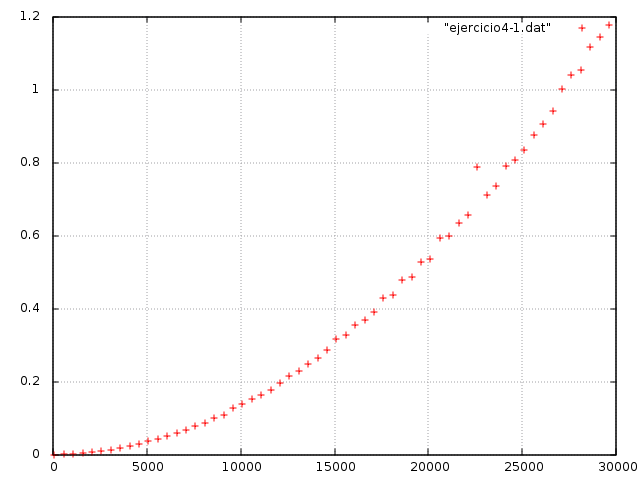
\includegraphics[width=0.4\textwidth]{1}
    }
    \qquad
    \subfigure[Ajuste] {
    \label{ajuste}
    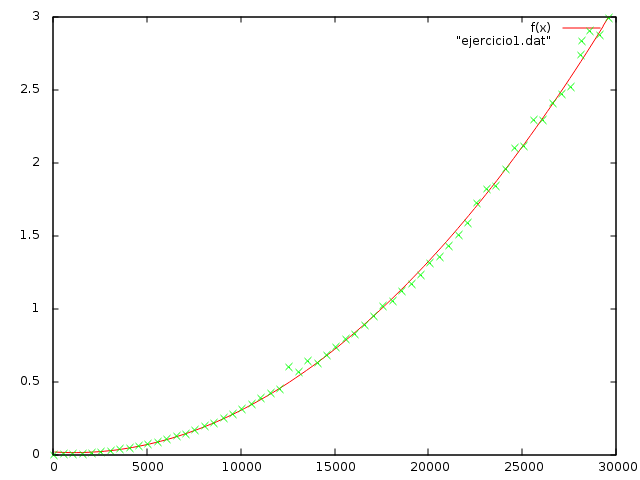
\includegraphics[width=0.4\textwidth]{2}
    }
    }
    \caption{Conteo y ajuste de un estudio a posteriori}
    \label{a-post}
    \end{figure}

    \subsubsection{\textcolor{YellowOrange}Enfoque empírico o \textit{a priori}}

    Consiste en la comprobación de la eficiencia del algoritmo antes de implementarlo, haciendo uso de técnicas como el \textit{\textcolor{YellowOrange}{estudio asintótico}} para ver el comportamiento del algoritmo cuando $n$ tiende a $\infty$

    Este tipo de estudios ahorra tiempo y recursos si el algoritmo es poco eficiente y nos evita errores como los que se pueden llegar en el estudio empírico.

    \begin{minted}[gobble=3, linenos]{c++}

        void Burbuja(int *v, int n) {
            for (int i=0; i<n-1; i++)
               for (int j=0; j<n-i-1; j++)
                    if (v[j]>v[j+1]) {
                       int aux = v[j];
                       v[j] = v[j+1];
                       v[j+1] = aux;
                    }
        }
    \end{minted}

    Para obtener la eficiencia del algoritmo de la Burbuja, analizaremos el código de dentro hacia fuera. Centrándonos en el \mint{c++}|if(v[j]>v[j+1]){...}| obtenemos que la eficiencia pertenece a O(1) por ser un conjunto de operaciones elementales. A continuación, se muestra la eficiencia del bucle \mint{c++}|for(int j=0; j<n-i-1; j++){...}| 

    \begin{displaymath}
        \sum_{j=0}^{n-i-2} 1
    \end{displaymath}

    Con esto, y gracias a la \hyperref[reglas_efic]{regla del producto} que aplicamos al ser bucles anidados, obtenemos que la eficiencia del algoritmo de la burbuja es:
    \begin{displaymath}
        \sum_{i=0}^{n-2}\sum_{j=0}^{n-i-2} 1
    \end{displaymath}

    Desarrollando esto, obtenemos:

    \begin{displaymath}
        \sum_{i=0}^{n-2}\sum_{j=0}^{n-i-2} 1 = \sum_{i=0}^{n-2}(n-i-1) = \sum_{i=0}^{n-2} n - \sum_{i=0}^{n-2} i - \sum_{i=0}^{n-2} 1 = 
    \end{displaymath}

    \begin{displaymath}
        n\sum_{i=0}^{n-2} 1 - \sum_{i=0}^{n-2} i - \sum_{i=0}^{n-2} 1 = n\cdot(n - 1) - \underbrace{(0 + 1 + 2 + ... + (n - 2))}_{Progresi\acute{o}n~aritm\acute{e}tica} - (n - 2 + 1) =
    \end{displaymath}

    \begin{displaymath}
        n\cdot(n-1) - \frac{(n-2)\cdot(n - 1)}{2} - (n - 1) = n^{2} - n - \frac{n^{2} - 3\cdot(n) + 2}{2} - n + 1 = 
    \end{displaymath}

    \begin{displaymath}
        n^{2} - \frac{n^{2}}{2} + \frac{n}{2} = f(n) \in O(n^2)
    \end{displaymath}

    \subsubsection{\textcolor{YellowOrange}Enfoque híbrido}

    Consiste en realizar un estudio a priori y luego completarlo con un estudio a posteriori, para demostrar gráficamente la veracidad del primer estudio.

    \section{\textcolor{YellowOrange}Notación asintótica}
    
    Estudia el comportamiento del algoritmo cuando el tamaño de las entradas, $n$, es lo suficientemente grande, sin tener en cuenta lo que ocurre para entradas pequeñas y obviando factores constantes.

    Existen varias notaciones asintóticas. Indican como crece $T$ para valores suficientemente grandes sin tener en cuenta las constantes. Entre más usaremos están:

    \begin{enumerate}[$\spadesuit$]
        \item $O(T)$: Orden de complejidad T.
        \item $\Omega(T)$: Orden inferior de T u omega de T.
        \item $\Theta(T)$: Orden exacto de T.
    \end{enumerate}
    
    \section{\textcolor{YellowOrange}Ordenes de eficiencia}

    Un algoritmo tiene un \textit{\textcolor{YellowOrange}{tiempo de ejecución de orden T(n)}}, para una función dada $T$, si existe una constate positiva $c$, y una implementación del algoritmo capaz de resolver cada caso del problema en un tiempo acotado superiormente por $c \cdot T(n)$, donde $n$ es el tamaño del problema considerado.

    Los oŕdenes más habituales y su inclusión en otros son los siguientes:

    \begin{enumerate}[$\spadesuit$]
        \item \textbf{\textcolor{YellowOrange}{Lineal}}: $n$
        \item \textbf{\textcolor{YellowOrange}{Cuadrático}}: $n^2$
        \item \textbf{\textcolor{YellowOrange}{Polinómico}}: $n^k$, con $k \in \aleph$
        \item \textbf{\textcolor{YellowOrange}{Logarítmico}}: $\log(n)$
        \item \textbf{\textcolor{YellowOrange}{Exponencial}}: $c^n$
    \end{enumerate}

    \begin{displaymath}
        O(1) \subset O(\log(n)) \subset O(n) \subset O(n\cdot \log(n)) \subset O (n \cdot (\log(n))^2) \subset O(n^{1.001...}) \subset O(n^2) \subset 
    \end{displaymath}
    \begin{displaymath}
        O(n^3) \subset ... \subset O(2^n) \subset O(n!) \subset O(n^n)
    \end{displaymath}

    \section{\textcolor{YellowOrange}Notación O-Mayúsucula}

    Una función $T(n)$ es $O(f(n))$ si existen constantes $n_0$ y $c$ tales que $T(n) \leq c\cdot f(n)$ para $n \geq n_0$. Es decir:
    \begin{displaymath}
        T(n) \subseteq O(f(n)) \Leftrightarrow \exists c \in \Re, \exists n_0 \in \aleph, \text{tal que } \forall n \geq n_0, T(n) \leq c\cdot f(n)
    \end{displaymath}

    Esta notación permite una \textit{\textcolor{YellowOrange}{flexibilidad en la notación}}. Emplearemos la notación $O(f(n))$ aun cuando en un número finito de valores de $n$, $f(n)$ sea negativa o no esté definida. Ej: $\frac{n}{log(n)}$

    Otro dato importante es que no todo es $O$ de todo. ¿Que significa esto? A continuación viene un ejemplo aclaratorio:

    \begin{displaymath}
        3^n \subsetneq c \cdot 2^n \quad \Rightarrow \quad c = \frac{3^n}{2^n}
    \end{displaymath}

    La notación $O(f(n))$ es un conjunto de funciones no una sola función, en la que no nos importa lo que pase con valores de $n$ pequeños. Este conjunto de funciones estarán acotadas superiormente por un mútliplo de $f$, por lo que nos quitamos las constantes.

    \begin{displaymath}
        \text{Esta función es aplicable para cualquier } f:\aleph \rightarrow \Re
    \end{displaymath}

    La notación $O-grande$ la usaremos para cuando tengamos un tiempo $t(n)$, encontrar la función $f$ más simple tal que $t \in O(f)$ y que más se aproxime asintóticamente.

    % \begin{center}
    %   \begin{tikzpicture}[scale=1]
    %   \begin{axis}[
    %       axis lines = left,
    %       xlabel = $n$,
    %       ylabel = {$R$},
    %   ]
    %   %Below the red parabola is defined
    %   \addplot [
    %       domain=0:20,
    %       samples=100,
    %       color=red,
    %   ]
    %   {x^2};
    %   \addlegendentry{$f(n)$}
    %   %Here the blue parabloa is defined
    %   \addplot [
    %       domain=0:20,
    %       samples=100,
    %       color=blue,
    %       ]
    %       {x*ln(x)^2};
    %   \addlegendentry{$g(n)$}
    %   \end{axis}
    %   \end{tikzpicture}
    % \end{center}

    \begin{figure}[!h]
    \centering
    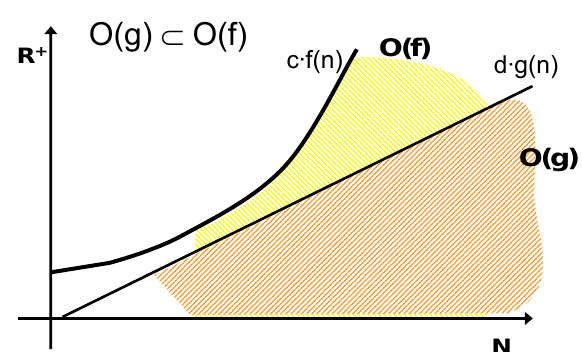
\includegraphics[width=0.8\textwidth]{3}
    \caption{Relación de orden entre $O(..)$}
    \label{Ogrande}
    \end{figure}
    \begin{displaymath}
        O(g) \leq O(f) \Leftrightarrow O(h) \subseteq O(f) \Leftrightarrow \forall t \in O(g), t \in O(f)
    \end{displaymath}

    \section{\textcolor{YellowOrange}Notación $\Omega$}

    Dada una función $f: \aleph \rightarrow \Re^+$, llamamos \textbf{\textcolor{YellowOrange}{omega de f}} al conjunto de todas las funciones de $\aleph$ en $\Re^+$ acotadas \textbf{\textcolor{YellowOrange}{inferiormente}} por un mútliplo real positivo de $f$, para valores $n$ suficientemente grandes.

    \begin{displaymath}
        \Omega(f) = \{t:\aleph \rightarrow \Re^+ \quad / \quad \exists c \in \Re^+, \quad \exists n_0 \in \aleph, \quad \forall n \ge n_0;\quad t(n) \ge c \cdot f(n) \}
    \end{displaymath}

    Esta notación se usa para establecer cotas inferiores del tiempo de ejecución, es decir, el mejor tiempo posible de ejecución del algoritmo.

    \section{\textcolor{YellowOrange}Notación exacta $\Theta$}

    Dada una función $f: \aleph \rightarrow \Re^+$, llamamos orden exacto de f al conjunto de todas las funciones de $\aleph en \Re^+$ que crecen igual que f, asintóticamente'y salvo constantes.

    \begin{displaymath}
        \Theta(f) = O(f) \cap \Omega(f) = \{ t:\aleph \rightarrow \Re^+ \quad \ \quad \exists c, d \in \Re^+, \exists n_0 \in \aleph, \forall n \ge n_0; c \cdot f(n) \ge t(n) \ge d \cdot f(n) \}
    \end{displaymath} 

    En resumen, si un algoritmo tiene un $t$ tal que $t \in O(f) \text{ y } t \in \Omega(f), \text{ entonces } t \in \Theta(f)$.

    %%%%%%%%%%%%%%%%%%%%%%%%%%%%%%%%%%%%%%%%%%%%%%%%%%%%%%%%%%%%%%%%%%%%%%%%%%
    % ENLACE AL APENDICE CON LOS EJERCICIOS RESUELTOS DE LA DIAPOSITIVA 38
    %%%%%%%%%%%%%%%%%%%%%%%%%%%%%%%%%%%%%%%%%%%%%%%%%%%%%%%%%%%%%%%%%%%%%%%%%%

    En el apéndice hay más ejemplos sobre las \hyperref[ejem_not]{notaciones asintóticas}.

    \section{\textcolor{YellowOrange}Propiedades de las notaciones asintóticas}

    \begin{enumerate}[$\spadesuit$]
        \item \textbf{\textcolor{YellowOrange}{Transitividad}}: Si $f \in O(g) \text{ y } g \in O(h)$ entonces $f \in O(h)$. Igual para $\Omega$. Por ejemplo:
        \begin{displaymath}
            2 \cdot n + 1\in O(n), \quad n \in O(n^2) \quad \Rightarrow \quad 2 \cdot n + 1\in O(n^2).
        \end{displaymath}
        \item \textbf{\textcolor{YellowOrange}{Inclusión}}: Si $f \in O(g)$ entonces $O(f) \subseteq O(g)$.
        \item \textbf{\textcolor{YellowOrange}{Relación pertenencia/contenido}}: Dadas $f,g:\aleph \rightarrow \Re^+$, se cumple:
            \begin{enumerate}[$\rightarrow$]
                \item $O(f) = O(g) \Leftrightarrow f \in O(g) \text{ y } g \in O(f)$
                \item $O(f) = \subseteq O(g) \text{ entonces } O(f) \subseteq O(g)$
            \end{enumerate}
        \item \textbf{\textcolor{YellowOrange}{Propiedad del máximo}}: Dadas $f,g: \aleph \rightarrow \Re^+, \qquad O(f+g) = O(max(f,g))$. Con $\Omega$ igual.
        \item \textbf{\textcolor{YellowOrange}{Relación límites/órdenes}}: Dadas $f,g: \aleph \rightarrow \Re^+$, se cumple lo siguinte:
            \begin{enumerate}[$\rightarrow$]
                \item $\lim_{n \rightarrow \infty} \frac{f(n)}{g(n)} \in \Re^+ \qquad O(f) = O(g)$
                \item $\lim_{n \rightarrow \infty} \frac{f(n)}{g(n)} = 0 \qquad O(f) \subset O(g)$
                \item $\lim_{n \rightarrow \infty} \frac{f(n)}{g(n)} = +\infty \qquad O(f) \supset O(g)$
            \end{enumerate}
    \end{enumerate}

    \section{\textcolor{YellowOrange}Otras observaciones}

    \subsubsection{\textcolor{YellowOrange}Notaciones con varios parámetros}

    El tiempo y la memoria consumidos pueden depender de muchos otros parámetros, por lo que se generarán notaciones con varios parámetros
    \begin{align*}
        f:\aleph^m \rightarrow \Re^+ \qquad (f:Nx\ldots^m\ldots x\aleph \rightarrow \Re^+)\\ \text{Orden de complejidad de } f(n_1, n_2, \ldots, n_m): O(f)
    \end{align*}

    Dada una función $f:\aleph^m\rightarrow \Re^+$, llamamos \textbf{\textcolor{YellowOrange}{orden de f}} al conjunto de todas las funciones de $\aleph^m$ en $\Re^+$ acotadas superiormente por un múltiplo real positivo de $f$, para valores de ($n_1,\ldots,n_m$) suficientemente grandes.

    \begin{align*}
        O(f) = \{t:\aleph^m \rightarrow \Re^+ \text{ / } \exists c \in \Re^+, \exists n_1, n_2, \ldots, n_m \in \aleph,\\ \forall k_1 \ge n_1. \forall k_2 \ge n_2, \ldots, \forall k_m \ge n_m;\\ (k_1,k_k,\ldots,k_m) \leq c \cdot f(k_1,k_k,\ldots,k_m)\}
    \end{align*}

    Algunos ejemplos de este tipo de notaciones son $O(n+m), \text{ } O(n^m), \text{ } O(n+2^m)$

    \subsubsection{\textcolor{YellowOrange}Notaciones condicionales}

    En algunos casos, es más interesante realizar el cálculo del tiempo solo para ciertos tamaños de entrada. Como ejemplo podríamos poner el algoritmo de la búsqueda binaria, en el que si $n$ es potencia de 2, el estudio se simplifica.

    \begin{minted}[linenos]{c++}
// La función devuelve la posición en la que se encuentra
// el elementoa buscar. Si no lo encuentra devuelve un -1

bool BusquedaBinaria (int x){
    int izda, dcha, centro;

    izda = 0;
    dcha = v.size() - 1;

    while(izda < dcha){

        centro = (izda + dcha) / 2;

        if(v[centro] == x)
            return centro;
        
        else{
            if(x > v[centro])
                izda = centro + 1;

            else
                dcha = centro
        }
    }

    return -1;
}
    \end{minted}

    Dada una función $f:\aleph \rightarrow \Re^+$, y $P:\aleph \rightarrow B$ llamamos \textbf{\textcolor{YellowOrange}{orden de f según P}} o condicionado a P al conjunto:
    \begin{align*}
        O(f|P) = \{t:\aleph \rightarrow \Re^+ \textbf{ / }
        \exists c \in \Re^+, \exists n_0 \in \aleph, \forall n \ge n_0;\\
        P(n) \Rightarrow t(n) \leq c \cdot f(n) \}
    \end{align*}

    De igual forma se aplica a la notación $\Omega$ y $\Theta$. Como ejemplos tenemos el tiempo para tamaños de entrada que sean potencias de 2 $t(n) \in O(f|n = 2^k)$ o para múltiplos de 2 $t(n) \in O(f | n = 2\cdot k) $

    \section{\textcolor{YellowOrange}Detalles frecuentes}
    \begin{enumerate}
        \item El orden de complejidad de un polinomio $a_n\cdot x^n+\ldots+a_1\cdot x + a_0$ es $O(x^n)$.
        \item $$\sum_{i=1}^{n} 1 \in O(n) \qquad \sum_{i=1}^{n} i \in O(n^2) \qquad \sum_{i=1}^{n} i^m \in O(n^{m+1})$$
        \item Independientemente de la base que tengan, los \textbf{\textcolor{YellowOrange}{logaritmos son del mismo orden}}. Por eso se omite la base.
        \item \textbf{\textcolor{YellowOrange}{Sumatorios}}: se pueden aproximar usando integrales, acontando superior e inferiormente.
        \item Para los casos \textbf{\textcolor{YellowOrange}{promedios}} hay que usar probabilidades.
    \end{enumerate}

    \section{\textcolor{YellowOrange}Cálculo del Orden de Eficiencia}

    \section{\textcolor{YellowOrange}Operación elemental}
    \label{ops_simples}
    Una operación elemental de un algoritmo es aquella cuyo tiempo de ejecución se puede acotar superiormente por una constante. Estas operaciones se contarán como $O(1)$. Entre estas operaciones están: 

    \begin{figure}
            
    \end{figure}    
    \begin{enumerate}[$\spadesuit$]
        \item Declaraciones.
        \item Asignaciones.
        \item Comparaciones simples.
        \item Operaciones aritméticas.
        \item Entrada y salida de datos básicos.
        \item Acceso a un array.
        \item etc.
    \end{enumerate}

    En muchas ocasiones, se producirán un número de repeticiones variables que dependen de $n$ de estas operaciones elementales. Por ejemplo:

    \begin{description}
        \item [Calcular el máximo $\rightarrow$ algoritmo]: $A$ es un vector con $n$ elementos y para calcular su máximo tenemos que hacer lo siguiente:
        \begin{displaymath}
            x = max{A[k], 0 \leq k < n}
        \end{displaymath}
        \item [Calcular el máximo $\rightarrow$ código]: el código en $C++$ sería:
\begin{minted}{c++}
    int A[MAX];     // O(1)
    int max = A[0]; // O(3)

    for(int i = 1; i < n; i++) // O(2); O(1); O(1)
        if(max < A[i])   // O(3)
            max = A[i];  // O(2)
\end{minted}
    \end{description}

    Hay que tener cuidado con algunas ``operaciones simples''. La eficiencia de algunas operaciones matemáticas pueden depender de la longitud de sus entradas, pero en la práctica se consideran que tienen un tamaño razonable. También hay que tener cuidado con las asignaciones que dependan de una función, ya que la asignación tendrá la eficiencia de la función. Por ejemplo:

\begin{minted}{c++}
    int tiempo;  // O(1)

    for(int i = 1; i < n; i++) O(2); O(1); O(1)
        tiempo = Hanoi(i);  // O(?) --> La eficiencia de esta asignación 
                            // dependerá de la eficiencia de la 
                            // función Hanoi(int i)
\end{minted}

    \subsection{\textcolor{YellowOrange}Reglas del cálculo del tiempo de ejecución}

    Para los cálculos sobre eficiencias, será necesario realizarlos de la siguiente forma:

    \begin{enumerate}[$\spadesuit$]
        \item Sentecias simples.
        \item Bucles.
        \item Sentecias condicionales.
        \item Bloques de sentencias.
        \item Llamadas a funciones.
        \item Funciones recursivas.
    \end{enumerate}

    \subsubsection{\textcolor{YellowOrange}Sentencias simples}

    Cualquier \hyperref[ops_simples]{sentencia simple} tendrá un tiempo $O(1)$ salvo que implique una llamada a una función.

    Este tipo de operaciones sumará 1 a $t(n) \rightarrow sumar~1$ por cada instrucción constante. Para un tiempo $t(n) \rightarrow sumar~(c_1, c_2,\ldots)$ por cada tipo de instrucción o grupo de instrucciones.

    \subsubsection{\textcolor{YellowOrange}Bucles}

    El tiempo de ejecución de un bucle es la suma del tiempo invertido en cada iteración. Este tiempo incluye el tiempo del cuerpo, la evaluación de la condición y la actualización.

    En un bucle donde las operaciones son iguales, el tiempo total será el producto del número de iteraciones por su tiempo de ejecución.

    \begin{description}
        \item [Bucles FOR]: se pueden expresar como un sumatorio con los límites del $FOR$ como límites del sumatorio.

        \begin{align*}
            \sum_{i=0}^{n} k = k\cdot n \qquad
            \sum_{i=a}^{b} k = k\cdot(b-a+1)\\
            \sum_{i=1}^{n} i = \frac{n\cdot(n+1)}{2} \qquad
            \sum_{i=a}^{b} r^i = \frac{r^{b+1}-r^a}{r-1}\\
            \sum_{i=1}^{n} i^2 \approx \int_{0}^{n} i^2 di = \frac{i^3}{3} ]_{0}^{n} = \frac{n^3}{3}\\
        \end{align*}

        Ejemplos:

        \begin{enumerate}
            \item Bucle sencillo para inicializar a 0 todos los componentes de un vector de tamaño arbitrario.

\begin{minted}[linenos]{c++}
int A[MAX]; //O(1)

for (int i=0; i<n; i++) //O(2); O(1); O(1)
      A[i] = 0;   //O(2)
\end{minted}
        En la primera vuelta del bucle, hemos gastado dos O(1) para inicializar la i y otro compararla con n. A partir de ahí, en el resto de las vueltas gastaremos una O(1) para comparar i con n, otra para incrementar i y dos más para igualar la componente del vector a cero:

\begin{displaymath}
(1+1) + 1 + \sum_{i=0}^{n-1}[(1+1) + (1+1)] = 3 + \sum_{i=0}^{n-1}4 = 3 + 4 \sum_{i=0}^{n-1}1 = 3 + 4n \in O(n)
\end{displaymath}

        A efectos prácticos, se suele dejar así:

\begin{displaymath}
\sum_{i=0}^{n-1} 1 = n
\end{displaymath}
        
        \item Bucles for anidados para el acceso a una matriz:

\begin{minted}[linenos, mathescape]{c++}

for (int i=0; i<n; i++) 
    for (int j=0; j<n; j++)   // $\sum_{j=0}^{n} 1 ~|~ \sum_{i=0}^{n} \sum_{j=0}^{n} 1 = \sum_{i=0}^{n} n \in O(n^2)$
        A[i][j] = 0; // O(1)          
\end{minted}

        \end{enumerate}
        \item [Bucles WHILE y REPEAT]: cota inferior y superior del número de ejecuciones.

        \label{eficiencia_sept2012}

        Ejercicio del examen de septiembre de 2012 de Estructura de Datos: ¿cuál es de mayor orden?
\begin{minted}[linenos]{c++}
int n, j;               int n, j;
int x=0, i=1;           int i=2, x=0;
do {                    do {
      j=1;                    j=1;
      while (j<=n)            while (j<=i)
      {                       {
            j *= 2;                 j*=2;
            x++;                    x++
      }                       }
} while (i<=n);         } while (i<=n)
\end{minted}

        El código de la izquierda repite su while $log_{2}(n+1)$ veces, y analizando el do while obtenemos que:
        \begin{displaymath}
        \sum_{i=1}^{n} log_{2} (n) + 1 = log_{2} (n) \sum_{i=1}^{n} 1 = nlog_{2}(n) + n \in O(nlog_{2}(n))
        \end{displaymath}

        El código de la derecha repite su while $log_{2} i$ veces, y analizándolo junto al do while obtenemos que:
        \begin{displaymath}
        \sum_{i=2}^{n} log_{2} i = log_{2} (2) + log_{2} (3) + \cdots + log_{2}(n) = log_{2} (2 \cdot 3 \cdots n) = log_{2} (n!) \in O(log_{2}(n!))
        \end{displaymath}

        El de mayor orden es el $nlog_{2} n$ ya que:
        \begin{displaymath}
        log_{2} (n!) = log_{2} 2 + log_{2} 3 + \cdots + log_{2} n \leq log_{2} n + log_{2} n + \cdots + log_{2} n = nlog_{2} n
        \end{displaymath}

    \end{description}

    \subsubsection{\textcolor{YellowOrange}Sentencias condicionales}

    Antes de entrar en detalle sobre las sentencias condicionales, hay dos reglas a tener en cuenta en el calculo de eficiencias de este tipo de sentencias:

    \begin{description}
    \label{reglas_efic}
        \item[Regla de la Suma]: Sean dos trozos de código, $c_1$ y $c_2$, independientes con eficiencia $T_1(n)$ y $T_2(n)$ respectivamente:

        \begin{displaymath}
T_{1}(n) + T_{2}(n) \in O(max(f(n),g(n))) \left\{ \begin{array}{ll}
T_{1}(n) \in O(f(n))\\
T_{2}(n) \in O(g(n))
\end{array} \right.
\end{displaymath}

    Un ejemplo de esto sería lo siguiente:

\begin{minted}[linenos]{c++}
int a=5, b=100;

if (a < b)        //O(1)
      cout << b;

else
      for (int i = 0; i < n; i++)   //O(n)
            A[i] = 0;

//O(max(1,n)) = O(n)
\end{minted}

    La eficiencia de este algoritmo es $O(1)$ y $O(n)$, que es $O(n)$.

    \item[Regla del producto]: Sean dos trozos de código, $c1$ y $c2$, dependientes con tiempos de ejecución $T_{1}(n)$ y $T_{2}(n)$ respectivamente:

\begin{center}
$T_{1}(n) \cdot T_{2}(n) \in O(f(n) \cdot g(n)) \left\{ \begin{array}{ll}
T_{1}(n) \in O(f(n))\\
T_{2}(n) \in O(g(n))
\end{array} \right.$
\end{center}

    La diferencia con la regla de la suma es que la suma de los dos trozos de código son \textbf{\textcolor{YellowOrange}{independientes}} (como por ejemplo, una sentencia if else) mientras que en la \hyperref[reglas_efic]{regla del producto}, son \textbf{\textcolor{YellowOrange}{dependientes}} (como por ejemplo, bucles anidados).


\begin{minted}[linenos]{c++}
void Ordena_Seleccion (const int *v, int n){
      for (int i=0; i<(n-1); i++)
            for (int j=i+1; j<n; j++)
                  if (v[j] < v[i]) //Todo este if es de orden O(1)
                        Intercambiar (v[i], v[j]);
}

void Intercambiar (int &a, int &b){
      //Toda esta funcion es de orden O(1)
      int aux = a;
      a = b;
      b = aux;
}
\end{minted}

    En la función Ordena Seleccion tenemos dos bucles anidados, en el segundo for tenemos:

\begin{displaymath}
\sum_{j=i+1}^{n-1} 1 = n - i -1
\end{displaymath}

    Tras aplicar la \hyperref[reglas_efic]{regla del producto} con el primer for, nos queda que:

\begin{displaymath}
\sum_{i=0}^{n-2} n - i - 1 = \sum_{i=0}^{n-2} n - \sum_{i=0}^{n-2} i - \sum_{i=0}^{n-2} 1 = n(n-1) - (n-2)\frac{(n-1)}{2} - (n-1) =
\end{displaymath}
\begin{displaymath}
= n(n-1) - \frac{(n-2)(n-1)}{2} - (n-1) = (n^{2}-1) - (\frac{n^{2}-3n+2}{2}) - n + 1 \in O(n^{2})
\end{displaymath}
    
    \end{description}

    Para el cálculo de la eficiencia de dos o varias sentencias condicioneales. se hará un análisis de cada parte condicional y se aplicará la \hyperref[reglas_efic]{regla de la suma} para obtener la eficiencia de este tipo de sentencias a partir del máximo de todos los bloques condicionales.

    \subsubsection{\textcolor{YellowOrange}Bloques de sentencias}

    Al igual que en el aprtado anterior, se aplicará la \hyperref[reglas_efic]{regla de la suma} para tomar el máximo de los tiempos de ejecución de cada una de las partes en que puede dividirse el bloque de sentencias.

    \subsubsection{\textcolor{YellowOrange}Llamadas a funciones}

    Si una determinada función $P$ tiene una eficiciencia de $O(f(n))$ con $n$ con la medida del tamaño de los argumentos, cualquier función que llame a $P$ tiene en la llamada una cota superior de eficiencia $O(f(n))$.

    Además de esto, hay que tener en cuenta varios aspectos importantes:

    \begin{itemize}
        \item Las asignaciones con diversas llamadas a función deben sumar las cotas de tiempo de ejecución de cada llamada.
        \item La misma consideración es válida para las condiciones de bucles y sentencias condicionales.
    \end{itemize}

    \section{\textcolor{YellowOrange}Funciones recursivas}

    Es normal que un algoritmo se base en procedimientos auxiliares, haga llamadas recursivas para tamaños menores o reduzca el tamaño del problema progesivamente.

    En el análisis, el tiempo $t(n)$ se expresa en función del tiempo para $t(n-1), t(n-2)...$. Es decir, con \textbf{\textcolor{YellowOrange}{ecuaciones de recurrencia}}.
    \label{hanoi}

    \begin{pseudocode}{Hanoi}{n,i,j,k}
            \IF N > 0 \\\THEN
                \BEGIN
                    Hanoi (n-1,i,k,j)\\
                    Mover (i,j)\\
                    Hanoi (n-1,k,j,i)\\
                \END\\
            \ELSE
                Mover(i,j)
        \end{pseudocode}

    La implementación de un algoritmo de forma recursiva puede ser que sea mucho más sencilla y rápida que hacer una función de forma iterativa. Pero, esto puede tener un serio problema y es que al realizar una función de forma recursiva se repitan muchas veces cálculos ya realizados anteriormente, se generan marcos de página con los mismos datos repetidos una y otra vez, pudiendo hacer que se salga de la pila del sistema.

    \subsection{\textcolor{YellowOrange}Tipos de recurrencias}

    Existen varios tipos de recurrencias, según la naturaleza de la función recursiva que tengan:

    \begin{enumerate}[$\spadesuit$]
        \item \textbf{\textcolor{YellowOrange}Ecuaciones lineales homogéneas}: Una recurrencia lineal homogénea de grado $k$ con coeficientes constantes es una expresión del tipo:

        \begin{displaymath}
            a_n + c_1a_{n-1} + c_2a_{n-2} + \cdots + c_ka_{n-k} = 0, c_i \in \Re, c_k \neq 0
        \end{displaymath}

        Para hallar una solución, tenemos que tener encontrar las condiciones iniciales $a_0, a_1, \cdots, a_{k-1}$, siendo $k$ el grado de la ecuación. Estas condiciones junto con la recurrencia, determinan la secuencia única

        \item \textbf{\textcolor{YellowOrange}Ecuaciones lineales no homogéneas}: Son aquellas relaciones de recurrencia que cumplen la siguiente expresión:

        \begin{displaymath}
            a_n + c_1a_{n-1} + c_2a_{n-2} + \cdots + c_ka_{n-k} = F(n), c_i \in \Re, c_k \neq 0
        \end{displaymath}

        \item \textbf{\textcolor{YellowOrange}Ecuaciones no lineales}: son aquellas relaciones de recurrencia que no cumplen ninguna de las expresiones anteriores. Para resolverlas, requieren realizar transformaciones hasta reducir la ecuación a una lineal.
    \end{enumerate}

    Para el cálculo de la eficiencia de estas recurrencias tendremos dos técnicas:

    \subsection{\textcolor{YellowOrange}Expansión de recurrencias}

    Consiste en aplicar varias veces la fórmula recurrente hasta encontrar una ``regularidad'' en la fórmula. Vamos a seguir con el ejemplo de las torres de Hanoi:
\begin{center}
    Fórmula general de las torres de Hanoi y caso base.
    \begin{displaymath}
        t(n) = \left\{ \begin{array}{ll}
1 & \textrm{si $n = 0$}\\
2\cdot t(n-1) + 1 & \textrm{si $n > 0$} \\
\end{array} \right.
    \end{displaymath}
    A continuación, vamos a extender la ecuación hasta encontrar esa ``regularidad'' y hallar así la fórmula general de la ecuación recurrente:
    \begin{align}
        t(n) = 2 \cdot t(n-1) + 1 = 2^2\cdot t(n-2) + 2 + 1\\
        = 2^3\cdot t(n - 3) + 4 + 2 + 1 = \ldots \\
        = 2^n\cdot t(n-n) + \sum_{i=0}^{n-1} 2^i = \sum_{i = 0}^{n} 2^i
        \\=
        2^{n+1} - 1 \in O(2`n) \Rightarrow \text{Horrible!! :(}
    \end{align}
\end{center}

\begin{minted}[linenos]{c++}
int E(int n){
    if(n == 1)
        return 0;
    else
        return E(n/2) + 1;
}
\end{minted}
\begin{displaymath}
    T(n) = \left\{ \begin{array}{ll}
1 & \qquad \textrm{si $n = 1$}\\
1 +  T(\frac{n}{2})& \qquad \textrm{si $n > 1$} \\
\end{array} \right.
\end{displaymath}

En este caso, al ir dividiendo entre dos el número de entradas, podemos concluir fácilmente que la eficiencia pertenece a $O(\log{n})$

Pinchando \hyperref[recurrencias]{aquí} se pueden ver más ejemplos con esta técnica.

\subsubsection{\textcolor{YellowOrange}Recurrencias no lineales}

A veces, por la naturaleza de la propia fórmula de recurrencia, su resolución de la forma tradicional puede ser muy complicado. Para este tipo de casos, existe una técnica conocida como \textbf{\textcolor{YellowOrange}{cambio de variable}}. Esta técnica consiste en buscar una transformación o cambio de variable para llegar a reducir la recurrencia no lineal a una lineal y así poder resolverla \verb|PARA ESE CAMBIO|. Después, habrá que deshacer los cambios de variable realizados y resolverla con la variable(s) original(es). Esto simplificará mucho los cálculos, haciendo más viable la resolución de la ecuación.

Por ejemplo:

\begin{displaymath}
    T(n) = \left\{ \begin{array}{ll}
1 & \qquad \textrm{si $n = 1$}\\
T(\frac{n}{2}) + n^2 & \qquad \textrm{si $n \ge 1$} \\
\end{array} \right.
\end{displaymath}

\begin{center}
    A continuación, vamos a ir desplegando la función poco a poco:
    \begin{displaymath}
        n = 2^m; n^2 = (2^m)^2 = 2^{2\cdot m} = 4^m
    \end{displaymath}
    \begin{displaymath}
        T(2^m) = T(2^{m-1}) + 4^m   
    \end{displaymath}
    \begin{displaymath}
        T(2^{m-2}) + 4^{m-1} + 4^m
    \end{displaymath}
    \begin{displaymath}
        \ldots \ldots \ldots \ldots \ldots \ldots
    \end{displaymath}
    Poco a poco, nos daremos cuenta de que la fórmula generla sigue este prototipo:
    \begin{displaymath}
        T(2^{m-i}) + [4^{m-(i-1)} + \cdots + 4^{m-1} + 4^m]
    \end{displaymath}
    \begin{displaymath}
        T(2^m) = T(1) + [4^1+\cdots+4^{m-2}+4^{m-1}+4^m]
    \end{displaymath}
    \begin{displaymath}
        \sum_{i = 0}^{m} 4^i = \frac{4^{m+1}-1}{4-1} = \frac{4}{3}4^m - \frac{1}{3}
    \end{displaymath}
    Una vez resuelta la recurrencia con el cambio de variable, deshacemos el cambio.
    \begin{displaymath}
        [4^m = n^2] = \frac{4}{3}n^2 - \frac{1}{3} \in O(n^2)
    \end{displaymath}
\end{center}

\subsection{\textcolor{YellowOrange}Ecuación característica}

El método anterior es válido para la resolución de recurrencias no lineales pero hasta un cierto límite, ya que la complejidad de estas funciones puede llegar de una complejidad tan alta, que su resolución por este método es prácticamente inviable.

Para solucionar este tipo de problemas, existe el método de la \textbf{\textcolor{YellowOrange}{ecuación característica}}.

La técnica de la ecuación característica se utiliza principalmente para resolver recurrencias no lineales, basándose en lo siguiente:

\begin{enumerate}[$\spadesuit$]
    \item Reducir las recurrencias no lineales a lineales homogéneas. En caso de que esto no sea posible, reducirlas primero a no homogéneas y luego a homogéneas.

    \item \textbf{\textcolor{YellowOrange}{Teorema fundamental del álgebra}}: según este teorema, todo polinomio de grado $k$ se tiene que:

        \begin{enumerate}[$\star$]
            \item Posee $k$ raíces (no necesariamente distintas).
            \item Puede factorizarse como un producto de $k$ monomios:
            \begin{displaymath}
                p(x) = \prod_{i = 1}^k(x-r_i)
            \end{displaymath}
            donde los $r_i$ pueden ser números complejos.
            \item Los $r_i$ son las únicas soluciones de la ecuación $p(x) = 0$.
        \end{enumerate}

    \item Dada cualquier raíz $r_i$ del polinomio característico tenemos que $p(r_i) = 0$ y por tanto $r_i^{n}$ es una solución de la recurrencia.

    \item Puesto que toda combinación lineal de soluciones es también solución se tiene que:
    \begin{displaymath}
        t_n = \sum_{i = 1}^k c_i\cdot r_i^n
    \end{displaymath}
    satisface la recurrencia para cualquier selección de constantes $c_1$, $c_2$,$\ldots$, $c_k$, \textbf{siempre y cuando todos los $r_i$ sean distintos}.

    \item Las $k$ constantes pueden determinarse a partir de las $k$ condiciones iniciales resolviendo un sistema de ecuaciones de tipo lineal.
    \begin{displaymath}
        \text{Ecuación característica}\rightarrow a_0x^k + a_1x^{k-1}+\ldots+a_k = 0
    \end{displaymath}
\end{enumerate}

Un ejemplo de uso de la ecuación característica para una recurrencia lineal homogénea es la resolución de Fibonacci:
\label{fibonacci_recursivo}

\begin{displaymath}
    f_n = \left\{ \begin{array}{ll}
n & \qquad \textrm{si $n = 0$, $n = 1$}\\
f_{n-1} + f_{n-2} & \qquad \textrm{en otro caso} \\
\end{array} \right.
\end{displaymath}

\begin{center}
    Planteamos la ecucación para el caso general:
    \begin{displaymath}
        f_n = f_{n-1} + f_{n-2}
    \end{displaymath}
    \begin{displaymath}
        f_n - f_{n-1} - f_{n-2} = 0
    \end{displaymath}
    Ahora planteamos la ecuación con el formato de la ecuación característica:
    \begin{displaymath}
        a_2x^n + a_1x^{n-1}+a_0x^{n-2} = 0
    \end{displaymath}
    \begin{displaymath}
        x^2 - x - 1 = 0
    \end{displaymath}
    Resolviendo esta ecuación obtenemos:
    \begin{displaymath}
        r_1 = \frac{1 \pm \sqrt{5}}{2} \rightarrow \text{Solución general}
    \end{displaymath}
    Para terminar de resolver la ecuación general y establecer el orden de eficiencia de la ecuación recurrente haremos lo siguiente:
    \begin{displaymath}
        f_n = c_1r_1^n + c_2r_2^n
    \end{displaymath}
    A continuación, resolveremos un sistema de ecuaciones utilizando las condiciones iniciales\footnote{En caso de no disponer de las condiciones iniciales suficientes, podemos usar la ecuación general para obtener todos los términos que sean necesarios}:
    \begin{displaymath}
        \left . \begin{array}{ll}
        f(n) = 0 & \qquad r_1^0c1 + r_2^0c2 = 0 \\
        f(n) = 1 & \qquad r_1^1c1 + r_2^1c2 = 1
        \end{array} \right \}
    \end{displaymath}
    \begin{displaymath}
        c_1 = \frac{1}{\sqrt{5}} \text{ y } c_2 = -\frac{1}{\sqrt{5}}
    \end{displaymath}
    \begin{displaymath}
        f_n = \frac{1}{\sqrt{5}}\cdot\left[ \left(\frac{1+\sqrt{5}}{2}\right)^n - \left(\frac{1-\sqrt{5}}{2}\right)^n\right] \in O\left(\left(\frac{1+\sqrt{5}}{2}\right)^n\right)
    \end{displaymath}
\end{center}

En el caso de las ecuaciones no homogéneas, la ecuación característica tiene ciertas peculiaridades. La ecuación característica de este tipo de ecuaciones cumple la siguiente expresión:

\begin{displaymath}
    a_0t_n + a_1t_{n-1}+\cdots+a_kt_{n-k} = b^np(n)
\end{displaymath}

Donde:
\begin{itemize}
    \item $b$ es una constante.
    \item $p(n)$ es un polinomio de $n$ de grado $d$.
    \item Ejemplo: $t_n - 2t_{n-1} = 3^n$
    \item El polinomio característico es: $p(x) = (a_0x^k + a_1x^{k-1}+\cdots+a_k)(x-b)^{d+1}$
    \item Se procede igual que en el caso homogéneo, salvo que las condiciones iniciales se obtienen de la propia recurrencia.
\end{itemize}

Aquí un ejemplo de la recurrencia no homogénea de las torres de Hanoi con la ecuación característica:

\begin{displaymath}
        T(n) = \left\{ \begin{array}{ll}
1 & \qquad \textrm{si $n = 1$}\\
2T(n - 1) + 1 & \qquad \textrm{si $n > 1$} \\
\end{array} \right.
\end{displaymath}
\begin{center}
Sacamos la ecuación general y aplicamos la ecuación característica:
\begin{displaymath}
    t_n - 2 t_{n-1} = 1 \Rightarrow (x - 2)(x - 1)
\end{displaymath}
Después de esto, despejamos las constantes y obtenemos la eficiencia del polinomio:
\begin{displaymath}
    t_n = c_12^n + c_21^n \rightarrow c_12^n + c_2 \in O(2^n)
\end{displaymath}
\end{center}

\subsubsection{\textcolor{YellowOrange}Ecuaciones no lineales}

Las ecuaciones de recurrencias no lineales son aquellas que, como su nombre indican, no tienen un crecimiento que siga un orden lineal. Esto significa que para aplicar las técnicas clásicas de resolución de recurrencias, tendremos que recurrir a trucos o herramientas que nos permitan realizar una transformación en esta recurrencia para conseguir que, de una ecuación cuya resolución es de un grado de complejidad muy alto, pase a ser algo que nos sea fácilmente reconocible y por tanto, podamos resolver sin mucho esfuerzo.

Un ejemplo de ecuación recurrente no lineal es el siguiente:

\begin{displaymath}
    T(n) = n\cdot T^2\left(\frac{n}{2}\right) \quad n > 1 \quad T(1) = 0
\end{displaymath}

Esta ecuación, como se puede ver, no tiene el típico crecimiento lineal $a_0x^k + a_1x^{k-1}+\ldots+a_k$ de las ecuaciones lineales homogéneas ni el de $a_0x^k + a_1x^{k-1}+\ldots+a_k = b^np(n)$ de una no lineal. Para resolverla haremos lo siguiente:

\begin{center}
    \begin{displaymath}
        T(n) = n\cdot T^2\left(\frac{n}{2}\right) \longrightarrow \log_2(T(n)) = \log_2
    \end{displaymath}
\end{center}

\chapter{\textcolor[rgb]{0.2,0.5,0.5}Algoritmos \textcolor[rgb]{0.2,0.5,0.5}Divide y \textcolor[rgb]{0.2,0.5,0.5}Vencerás}

\textbf{\textcolor[rgb]{0.2,0.5,0.5}{Divide y vencerás}} es una técnica para el diseño de algoritmos que consiste en descomponer el caso que haya que resolver en un cierto número de subcasos más pequeños del mismo problema, resolver sucesiva e independientemente todos los subcasos y combinar después las soluciones obtenidas de esta manera para obtener la solución del caso original.

\section{\textcolor[rgb]{0.2,0.5,0.5}Esquema general}

El esquema general del los algoritmos tipo divide y vencerás sigue algo así:

\begin{minted}[linenos]{pascal}
procedure DivideVenceras (p: problema)
    Dividir(p, p_1, p_2, ..., p_k)
    
    for i := 1 .. k
        s_i := Resolver(p_i)
    end
    
    solucion:=Combinar(s_1, s_2, ..., s_k)
end
\end{minted}

Normalmente, este tipo de problemas se solucionan realizando llamadas recursivas al mismo algoritmo, aunque no necesariamente debe ser así. También se pueden resolver utilizando algoritmos iterativos. La ventaja de estos sobre los recursivos es que no realiza llamadas a la misma función ocupando espacio en la pila y realizando los mismos cálculos. La desventaja es que su implementación es más complicada que uno recursivo.

Existen una gran cantidad de problemas que se puede resolver por divide y vencerás como pueden ser:

\begin{enumerate}[$\star$]
    \item Problema de las torres de \hyperref[hanoi]{Hanoi}.
    \item Problema de la sucesión de \hyperref[fibonacci_recursivo]{Fibonacci}.
\end{enumerate}

La técnica de \textbf{\textcolor[rgb]{0.2,0.5,0.5}divide y vencerás} se aplica en campos tan distintos como pueden ser las estrategias militares, demostraciones lógicas y matemáticas, diseño modular de programas, de circuitos...

\section{\textcolor[rgb]{0.2,0.5,0.5}Fundamentos de los algoritmos divide y vencerás}

Lo más común es que estos algoritmos tengan un \textbf{\textcolor[rgb]{0.2,0.5,0.5}{esquema recursivo}}, con división en 2 subproblemas y datos almacenados en una tabla entre las posiciones $p$ y $q$.

\begin{minted}[linenos]{pascal}
procedure DivideVenceras(p,q: indice)
var m: indice
    if Pequenio(p,q) then
        solucion:=SolucionDirecta(p,q)
    else
        m:=Dividir(p,q)
        solucion:=Combinar(DivideVenceras(p,m),
                           DivideVenceras(m+1,q))
    end
end
\end{minted}
\begin{center}
\begin{tabular}{|c|c|c|c|c|c|c|c|c|c|c|}
\hline
&&&&&&&&&&\\
\hline
\end{tabular}
\end{center}
\begin{center}
\begin{tabular}{cccccccccc}
&&$\mathbf{\uparrow}$&&&&$\mathbf{\uparrow}$&&\\
&&p&&&&q&&\\
\end{tabular}
\end{center}

\subsection{\textcolor[rgb]{0.2,0.5,0.5}Aplicación}
Para poder aplicar la técnica de divide y vencerás, temenos que encontrar la forma de definir las \textbf{\textcolor[rgb]{0.2,0.5,0.5}{funciones genéricas}}:

\begin{enumerate}[$\star$]
    \item \textbf{\textcolor[rgb]{0.2,0.5,0.5}{Pequeño}}: Determina cuándo el problema es pequeño para aplicar la resolución directa.
    \item \textbf{\textcolor[rgb]{0.2,0.5,0.5}{SoluciónDirecta}}: Método alternativo de resolución para tamaños pequeños.
    \item \textbf{\textcolor[rgb]{0.2,0.5,0.5}{Dividir}}: Función para descomponer un problema grande en subproblemas.
    \item \textbf{\textcolor[rgb]{0.2,0.5,0.5}{Combinar}}: Método para obtener la solución al problema original, a partir de las soluciones de los subproblemas.
\end{enumerate}

Para poder aplicar esta técnica debemos definir todas y cada una de las funciones genéricas, debemos aplicar un razonamiento inductivo.

\subsubsection{\textcolor[rgb]{0.2,0.5,0.5}Requisitos}

Antes de aplicar divide y vencerás, tienen que cumplirse una serie de requisitos:

\begin{enumerate}[$\star$]
    \item Se necesita un \textbf{\textcolor[rgb]{0.2,0.5,0.5}{método}} (más o menos \textbf{\textcolor[rgb]{0.2,0.5,0.5}{directo}}) para resolver problemas de pequeño tamaño.

    \item El problema original debe poder dividirse fácilmente en un conjunto de subproblemas, del \textbf{\textcolor[rgb]{0.2,0.5,0.5}{mismo tipo}} que el problema original, pero deben tener una resolución menos costosa.

    Normalmente, estos subproblemas serán de tamaño parecido, siendo, como mínimo, dos subproblemas. Si sólo tenemos un subproblema, entonces aplicamos técnicas de \textbf{\textcolor[rgb]{0.2,0.5,0.5}{reducción}} o \textbf{\textcolor[rgb]{0.2,0.5,0.5}{simplificación}}. Por ejemplo: cálculo del \hyperref[ej_factorial]{factorial}.

    \item Los subproblemas deben ser \textbf{\textcolor[rgb]{0.2,0.5,0.5}{disjuntos}}, es decir, la solución de un problema debe obtenerse de forma independiente a los otros subproblemas.

    \item Se necesita disponer de un método para \textbf{\textcolor[rgb]{0.2,0.5,0.5}{combinar}} los resultados de los subproblemas.
\end{enumerate}

A continuación vamos a ver dos ejemplos donde \textbf{no} se debe usar divide y vencerás, y otro donde sí es interesante usar esta técnica, ya que supone una mejora al algoritmo clásico:

\begin{description}
    \item [Problema del viajante]: El problema del viajante es un problema de tipo \hyperref[np_prob_def]{NP duro} que responde a la pregunta de cuál es la ruta más corta posible que visita cada ciudad exactamente una vez y regresa a la ciudad origen. Este problema tiene ua resolución trivial con 3 nodos, pero con más surgen los siguientes problemas:
    \begin{enumerate}[$\star$]
        \item Hay que descomponer el problema en subproblemas más pequeños, pero, ¿por dónde?.
        \item Los subproblemas deben ser disjuntos, algo que en este caso, parece difícil.
        \item Y la combinación de los resultados de los subproblemas no es posible en este caso.
    \end{enumerate}
    \item [Ordenar un vector]: Uno de los algoritmos más conocidos para la ordenación de un vector es \textbf{\textcolor[rgb]{0.2,0.5,0.5}{MergedSort}} que para ordenar el vector, realiza una serie de divisiones de forma recursiva hasta llegar al caso base, donde empieza a ordenar y reconstruir una solución, mezclando posteriormente las soluciones para componer la solución final.

    La ecuación recurrente de este algoritmo es la siguiente:
    \label{ef_merge}
    \begin{displaymath}
        T(n) \left\{ \begin{array}{ll}
        \Theta(1)\qquad \qquad \qquad \text{si } n = 1 \\
        2T\left(\frac{n}{2}\right) + \Theta(n) \quad \text{  si } n > 1\\
        \end{array} \right.
    \end{displaymath}
    \begin{center}
        En este caso, la eficiencia de la ecuación $T(n) = 2\cdot T(\frac{n}{2}) + \Theta(n)$ viene definida por las dos llamadas al procedimiento recursivo y el tiempo promedio que viende de la división y combinación de los resultados.

        En definitiva $T(n) \in \Theta(n\log n)$.
    \end{center}

    Como se puede ver, la versión con divide y vencerás es mucho mejor que la versión clásica, realizando dos llamadas recursivas al algoritmo con $\frac{n}{2}$ datos y combinando los resultados.
\end{description}

Una de las características de los algoritmos aplicando la técninca Divide y Vencerás es que, además de ser los subproblemas de un tamaño parecido e independientes, los datos de entrada para el cálculo del subproblema no necesitan ser una fracción de tamaño fijo para cada división, sino que pueden ser tan solo unos elementos menos que el problema original (versión recursiva de la búsqueda lineal).

En general, si se realizan $k$ llamadas recursivas de tamaño $\frac{n}{b}$, y la división y combinación de la solución a los subproblemas requieren $f(n) = d\cdot n^p \in O(n^p)$, entonces:
\begin{center}
    \begin{displaymath}
        t(n) = a \cdot t\left(\frac{n}{b}\right) + d\cdot n^p   
    \end{displaymath}
    Suponiendo $n = b^k \Rightarrow k = \log_b n$: $t(b^k) = a\cdot t(b^{k-1}) + d\cdot b^{pk}$, se puede deducir que:

    \begin{displaymath}
        t(n) \left\{ \begin{array}{lll}
        O(n^{\log_b a}) \qquad \qquad \qquad \text{si } a > b^p \\
        O(n^p \cdot \log n) \quad \text{  si } a = b^p \\
        O(n^p) \qquad \qquad \text{ si } a < b^p 
        \end{array} \right\} \text{\large{\textbf{Fórmula Maestra}}}
    \end{displaymath}
\end{center}

A continuación, un par de ejemplos ilustrativos:
    \begin{enumerate}[$\spadesuit$]
        \item Si dividimos en 2 trozos de tamaño $\frac{n}{2}$, con $f(n) \in O(n)$:
        \begin{center}
            $a = b = 2$
            $t(n) \in O(n\cdot\log n)$
        \end{center}
        \item Realizamos 4 llamadas recursivas con trozos de tamaño $\frac{n}{2}$, con $f(n) \in O(n)$;
        \begin{center}
            $a = 4$; $b = 2$
            $t(n) \in O(n^{\log_24}) = O(n^2)$
        \end{center}
    \end{enumerate}

\section{\textcolor[rgb]{0.2,0.5,0.5}Método General DV}

\begin{minted}[linenos]{pascal}
procedure DV(x)
    if x es suficientemente pequenio then
        return ad hoc(x)
    desconmponer x en casos más pequenios x_1 .. x_l
    for i = 1 .. l y_i = DV(x_i)
    recombinar los y_i para obtener una solucion y de x
    return y    
\end{minted}

\begin{itemize}
    \item $l$ es el número de subcasos.
    \item si $l=1$ hablamos de reducción.
    \item $ad$ $hoc(x)$ es un algoritmo básico.
\end{itemize}

Las principales características de Divide y Vencerás son:
\begin{enumerate}[$\spadesuit$]
    \item Los subproblemas en los que se dividen el problema original.
    \item Cada uno de los subproblemas se resuelve de forma independiente.
    \item No existe solapamiento entre los subproblemas.
\end{enumerate}

La técnica de Divide y Vencerás es una técnica muy potente para resolver problemas complejos, pero que conlleva una serie de riesgos. Un mal uso de esta técnica, puede generar que el coste de la solución sea mucho peor que una solución clásica. Pero, para que esta técnica funcione, deben darse las siguientes condiciones:

\begin{enumerate}[$\spadesuit$]
    \item Debe hacerse un estudio exhaustivo para decidir cuándo utilizar el algoritmo \textit{\textcolor[rgb]{0.2,0.5,0.5}{ad hoc}}, para no aplicar la recursividad hasta el límite. Es decir, calcular el \textbf{\textcolor[rgb]{0.2,0.5,0.5}{umbral de recursividad}}.

    \item La descomposición del problema en subproblemas y recombinar las soluciones parciales debe poder hacerse de forma eficiente ($O(1)$, $O(n)$).

    \item Cada uno de los subproblemas deben tener de forma aproximada el mismo tamaño.
\end{enumerate}

\section{\textcolor[rgb]{0.2,0.5,0.5}Determinación del Umbral}

Es difícil hablar del umbral \textcolor[rgb]{0.2,0.5,0.5}{$n_0$} si no se trata con implementaciones, ya que gracias a ellas, se pueden determinar las constantes ocultas que permiten afinar el cálculo de este umbral. Este umbral no es único, pero para cada tipo de implementación, sí que lo es.

De partida, no existen restricciones sobre qué valor puede llegar a tener \textcolor[rgb]{0.2,0.5,0.5}{$n_0$}, así que en un principio, \textcolor[rgb]{0.2,0.5,0.5}{$n_0$} puede variar desde 0 a infinito:

\begin{enumerate}
    \item El umbral infinito supone que nunca se aplica el algoritmo \textcolor[rgb]{0.2,0.5,0.5}{Divide y Vencerás} de forma efectiva, por lo que siempre se está aplicando el algoritmo básico o clásico.
    \item Si $n_0 = 1$, quiere decir que estamos en el caso contrario. Es decir, que siempre se está aplicando el algoritmo \textcolor[rgb]{0.2,0.5,0.5}{Divide y Vencerás}, aplicando siempre la recursividad y el algoritmo básico sólo se aplica una vez.
\end{enumerate}

Un ejemplo de ello es la multiplicación de enteros largos, donde
\begin{equation*}
t(n) = 
\begin{cases}
h(n) & \textit{si } n \leq n_0, \\
3t(\frac{n}{2}) + g(n) & \textit{otro caso}
\end{cases}
\end{equation*}

con $h(n) \in O(n^2)$, $g(n) \in \Theta(n)$.

¿Cuál es el valor ótpimo para $n_0$?

Una implementación concreta $h(n) = n^2$ y $g(n) = 16n (\mu s)$, y un caso de tamaño $n=5000$.

Las dos posibilidades extremas nos llevan a:

\begin{enumerate}
    \item $n_0 = 1$, $t(n) = 41sg$.
    \item $n_0 = \infty$, $t(n) = h(n) = 25sg$.
\end{enumerate}

Como se puede observar, existen unas diferencias muy significativas entre un caso u otro, por lo que \textbf{¿cómo podremos determinar el valor óptimo del umbral?}

Para ello, al igual que a la hora de determinar la eficiencia de un algoritmo, tenemos trés métodos: \textbf{\textcolor[rgb]{0.2,0.5,0.5}{Experimental}, \textcolor[rgb]{0.2,0.5,0.5}{Teórico}} e \textbf{\textcolor[rgb]{0.2,0.5,0.5}{Híbrido}}

\subsection{\textcolor[rgb]{0.2,0.5,0.5}Método experimental}

Consiste en implementar el algorítmo básico ($AB$) y el algorítmo Divide y Vencerás ($DV$), resolver para distintos valores de $n$ con ambos algoritmos y esperar a que conforme $n$ aumente, el tiempo del algorítmo básico vaya aumentando asintóticamente, y el de $DV$ vaya disminuyendo.


\begin{center}
    \begin{tikzpicture}[scale=1]
    \begin{axis}[
        axis lines = left,
        % xlabel = $n$,
        % ylabel = {$R$},
    ]
    %Below the red parabola is defined
    \addplot [
        domain=0:2,
        samples=200,
        color=red,
    ]
    {x^2};
    \addlegendentry{$f(n)$}
    %Here the blue parabloa is defined
    \addplot [
        domain=0:10,
        samples=200,
        color=blue,
        ]
        {sqrt(x)};
    \addlegendentry{$g(n)$}
    \end{axis}
    \end{tikzpicture}
\end{center}

\subsection{\textcolor[rgb]{0.2,0.5,0.5}Método teórico}

La idea del enfoque experimental se traduce a lo siguiente:

\begin{equation*}
t(n) = 
\begin{cases}
h(n) & \textit{si } n \leq n_0, \\
3t(\frac{n}{2}) + g(n) & \textit{si } n> n_0
\end{cases}
\end{equation*}

Teniendo la ecuación de recurrencia, el umbral se traduce en averiguar cuándo coinciden los tiempos de los dos algoritmos. Es decir
\begin{displaymath}
    h(n) = t(n) = 3\left(h\frac{n}{2}\right) + g(n); n = n_0
\end{displaymath}

\subsection{\textcolor[rgb]{0.2,0.5,0.5}Método híbrido}

Para una implementación concreta, tenemos que:

\begin{enumerate}
    \item Calcular las constantes ocultas utilizando un enfoque emírico.
    \item Calcular el umbral, utilizando el criterio seguido para el umbral teórico.
    \item Probar valores alrededor del umbral teórico, es decir, probar valores que se alojen en la zona conocida como \textit{\textcolor[rgb]{0.2,0.5,0.5}{umbral de tanteo}} para determinar el umbral óptimo.
    \item El inconveniente está en que las constantes ocultas, son poco importantes para tamaños de $n$ grandes.
\end{enumerate}

\section{\textcolor[rgb]{0.2,0.5,0.5}Algoritmos de Ordenación}

Los algoritmos de ordenación son una de las aplicaciones donde el enfoque divide y vencerás funciona mejor. La ordenación es una de las tareas más frecuentemente realizadas.

Estos algoritmos, reciben una colección de registros a ordenar. Cada uno de estos registros, contiene un campo \textbf{\textcolor[rgb]{0.2,0.5,0.5}{clave}} por el que se ordenarán los registros, siendo esta clave de cualquier tipo (numérica, alfanumérica...) para el que exista una función de comparación.

La clave debe ser de un tipo lo suficientemente grande como para que haya una relación de orden lineal entre las claves.

Se supondrá que todos los registros tienen una función \textit{\textbf{\textcolor[rgb]{0.2,0.5,0.5}{clave()}}} que devuelve el valor que tiene su clave.

También se supondrá que está definida la función \textit{\textbf{\textcolor[rgb]{0.2,0.5,0.5}{swap()}}}, que se encarga de intercambiar la posición de dos registros cualesquiera.

\subsection{\textcolor[rgb]{0.2,0.5,0.5}Definición}

Dado un conjunto de registros $r_1$, $r_2$, $\ldots$, $r_n$ con valores clave $k_1$, $k_2$, $\ldots$, $k_n$ respectivamente, fijar los registros con algún orden $s$ tal que los registros $r_{s1}$, $r_{s2}$, $\ldots$, $r_{sn}$ tengan claves que obedezcan la propiedad $k_{s1}$, $k_{s2}$, $\ldots$, $k_{sn}$

En resumen, este problema trata de fijar un conjunto de registros de forma que los valores de sus claves estén en \textit{\textbf{\textcolor[rgb]{0.2,0.5,0.5}{orden creciente}}}.

Hay que tener en cuenta que esta definición permite la existencia de valores clave repetidos. Cuando esto ocurre, puede ser interesante mantener el orden en el que estos elementos aparecían en el conjunto inicial.

Se denomina \textbf{\textcolor[rgb]{0.2,0.5,0.5}{estable}} al algoritmo de ordenación que \textit{mantiene el orden relativo en que ocurren los registros con clave repetida en la entrada}.

\subsection{\textcolor[rgb]{0.2,0.5,0.5}Algoritmos de Ordenación Lentos}

Son algoritmos de ordenación por cambio, con una eficiencia media pertenciente a $\Theta(n^2)$, sencillos de implementar, pero, con la gran pega de que se comportan muy mal cuando el tamaño de $n$ es muy grande.


\subsubsection{\textcolor[rgb]{0.2,0.5,0.5}Ordenación de la burbuja}

 A la izquierda se va dejando un subvector ordenado. Desde el final y hacia atrás, se van comparando los elementos dos a dos y se deja a la izquierda el más pequeño (intercambiándolos). Para ello, vamos fijando el inicio del subvector derecho con un contador, recorremos el subvector de la derecha desde el final hasta el principio con un contador i y si v[i] menor que v[i-1] se intercambian.

 Una posible implementación de este algoritmo es:

 \begin{minted}[linenos]{c++}
void Ordena_Burbuja (){
  bool cambio;

  for (izda = 0; izda < total_utilizados && cambio; izda++){

    cambio = false;
    for (i = total_utilizados-1; i>izda; i--)
        if (vector_privado[i] < vector_privado[i-1]){
              swap(i, i-1);
              cambio = true;
        }
    }
}
\end{minted}

\subsubsection{\textcolor[rgb]{0.2,0.5,0.5}Ordenación por inserción}

La búsqueda por inserción procesa secuencialmente la lista de registros, manteniendo una lista ordenada con los registros procesados.

Cada uno de los registros se inserta en la posición correcta dentro de la lista ordenada cuando le toca.

El cuerpo del algoritmo está formado por dos bucles $for$ anidados, donde el externo se ejecuta $n-1$ veces. El bucle interno depende del número de claves en la parte ordenada que son menores (o mayores) que la clave que queremos ordenar.

En el peor de los casos, cada registro debe moverse hasta el principio del vector ($i$ comparaciones por pasada), lo que implica un coste de:
\begin{displaymath}
    \sum_{i=1}^n i = \Theta (n^2)
\end{displaymath}

En el mejor caso, las claves estarán ordenadas de menor a mayor y solo habrá que realizar 1 comparación por pasada.
\begin{displaymath}
    \sum_{i=1}^n 1 = \Theta (n)
\end{displaymath}

Como se puede ver, el \textit{\textbf{\textcolor[rgb]{0.2,0.5,0.5}{mejor caso}}} es muchísimo más rápido que el \textit{\textbf{\textcolor[rgb]{0.2,0.5,0.5}{peor caso}}}, que suele ser una \textbf{\textcolor[rgb]{0.2,0.5,0.5}{indicación de mayor confianza}} del tiempo ``típico'' que tarda el proceso en realizarse.

Puede haber situaciones en los que este algoritmo se comporte como en el mejor caso, como puede ser que una lista ordenada esté ligeramente desordenada. 

%%%%%%%%%%%%%%%%%%%%%%%%%% HAY QUE PONER UN ENLACE %%%%%%%%%%%%%%%%%%%%%%%%%%

Esto lo aprovechan algunos algoritmos de ordenación para mejorar su rendimiento, como pueden ser \textbf{\textcolor[rgb]{0.2,0.5,0.5}{ShellShort}} o \textbf{\textcolor[rgb]{0.2,0.5,0.5}{QuickSort}}.

Entonces, ¿cuál es el coste del caso medio? El número de iteraciones del bucle interno depende de lo ``desordenado'' que se encuentre el registro. Es decir, se darán tantas pasadas como 



\begin{minted}[linenos]{c++}

void Ordena_por_Insercion (vector<int> & v){    
    int tam = v.size();

    int izda, i; 

    for (izda = 2; izda <= tam; izda++) {
        
        int aux = v[izda];
        
        for (i=izda; i > 0 && aux < v[i-1]; i--)
            v[i]  = v[i-1]; 
                            
        v[i] = aux; 
    }
}
\end{minted}

\subsubsection{\textcolor[rgb]{0.2,0.5,0.5}Ordenación por selección}

\begin{minted}[linenos]{c++}
    
void Ordena_Seleccion (const int *v, int n){
  for (int i=0; i<(n-1); i++)
    for (int j=i+1; j<n; j++)
      if (v[j] < v[i]) //Todo este if es de orden O(1)
        swap (v[i], v[j]);
}
\end{minted}

\subsection{\textcolor[rgb]{0.2,0.5,0.5}Algoritmos de Ordenación Rápidos}

Son algoritmos más complejos y mucho más rápidos que los anteriores, cuando el tamaño de $n$ es muy grande. Algunos de ellos se basan en la recursividad, hasta cierto punto, donde para $n$ pequeños, llaman a otros algoritmos que se comportan mejor en estos casos.

\subsubsection{\textcolor[rgb]{0.2,0.5,0.5}Algoritmo por montículos (heapsort)}

Se basa en la simulación de la inserción y borrado en un árbol parcialmente ordenado \textit{\textcolor[rgb]{0.2,0.5,0.5}{APO}}, simulado sobre un vector. Su funcionamiento interno es el siguiente: 

% \documentclass[10pt,a4paper,spanish]{article}

% \usepackage[spanish]{babel}
% \usepackage[utf8]{inputenc}
% % \usepackage{amsmath, amsthm}
% \usepackage{amsfonts, amssymb, latexsym}
% \usepackage[usenames, dvipsnames]{color}
% \usepackage{colortbl}
% \usepackage{multirow}
% \usepackage[all]{xy}
% \usepackage{xcolor}

% \begin{document}

Ordenar los siguientes elementos:

\begin{displaymath}
\{5, 700, 46, 89, 6, 3\}
\end{displaymath}

En primer lugar, insertamos los elementos en el árbol y en el heap:

\begin{minipage}{0.3\textwidth}
\[\begin{xy}
% ,(32,-8)*+=<20mm>[]\txt<2cm>{RSI(3)}
,(0,0)*+=<10mm>[]\txt<2cm>{5}
% ,(7,5)*+=<10mm>[]\txt<2cm>{$h=3$}
,(-10,-10)*+=<10mm>[]\txt<2cm>{700}
,(10,-10)*+=<10mm>[]\txt<2cm>{46}
,(-15,-20)*+=<10mm>[]\txt<2cm>{89}
% ,(-5,-20)*+=<10mm>[]\txt<2cm>{56}
% ,(5,-20)*+=<10mm>[]\txt<2cm>{13}
% ,(15,-20)*+=<10mm>[]\txt<2cm>{4}
% ,(-20,-30)*+=<10mm>[]\txt<2cm>{35}
% ,(-15,-30)*+=<10mm>[]\txt<2cm>{13}
% ,(-10,-30)*+=<10mm>[]\txt<2cm>{56}
% ,(0,-30)*+=<10mm>[]\txt<2cm>{56}
% ,(10,-30)*+=<10mm>[]\txt<2cm>{13}
% ,(20,-30)*+=<10mm>[]\txt<2cm>{5}
%,(-5,-30)*+=<10mm>[]\txt<2cm>{7}
% ,(10,-30)*+=<10mm>[]\txt<2cm>{13}
% ,(-5,-40)*+=<10mm>[]\txt<2cm>{10}

% \ar@{->} (5,3);(0,1)
\ar@{->} (15,-10);(30,-10)
\ar@{-} (0,-2);(-10,-9) % raiz al hijo izq
\ar@{-} (0,-2);(9,-8) % raiz al hijo dcha
\ar@{-} (-10,-12);(-15,-18) % 5 al 3
% \ar@{-} (10,-12);(5,-18) % 14 al 12
% \ar@{-} (10,-12);(15,-18) % 14 al 15
% \ar@{-} (-15,-22);(-20,-28)
% \ar@{-} (-15,-22);(-15,-28)
% \ar@{-} (-10,-12);(-5,-18) % 5 al 7
% \ar@{-} (-5,-22);(-10,-28) % 7 al 6
% \ar@{-} (-5,-22);(0,-28)
% \ar@{-} (5,-22);(10,-28)
% \ar@{-} (15,-22);(10,-28) % 15 al 14
% \ar@{-} (15,-22);(20,-28)
% \ar@{-} (-5,-22);(-5,-28) % 7 al 8
% \ar@{-} (0,-32);(-5,-38) % 12 al 13
\end{xy}\]
\end{minipage}
\begin{minipage}{0.5\textwidth}
\[\begin{xy}
% ,(32,-8)*+=<20mm>[]\txt<2cm>{RSI(3)}
,(0,0)*+=<10mm>[]\txt<2cm>{5}
% ,(7,5)*+=<10mm>[]\txt<2cm>{$h=3$}
,(-10,-10)*+=<10mm>[]\txt<2cm>{89}
,(10,-10)*+=<10mm>[]\txt<2cm>{46}
,(-15,-20)*+=<10mm>[]\txt<2cm>{700}
% ,(-5,-20)*+=<10mm>[]\txt<2cm>{56}
% ,(5,-20)*+=<10mm>[]\txt<2cm>{13}
% ,(15,-20)*+=<10mm>[]\txt<2cm>{4}
% ,(-20,-30)*+=<10mm>[]\txt<2cm>{35}
% ,(-15,-30)*+=<10mm>[]\txt<2cm>{13}
% ,(-10,-30)*+=<10mm>[]\txt<2cm>{56}
% ,(0,-30)*+=<10mm>[]\txt<2cm>{56}
% ,(10,-30)*+=<10mm>[]\txt<2cm>{13}
% ,(20,-30)*+=<10mm>[]\txt<2cm>{5}
%,(-5,-30)*+=<10mm>[]\txt<2cm>{7}
% ,(10,-30)*+=<10mm>[]\txt<2cm>{13}
% ,(-5,-40)*+=<10mm>[]\txt<2cm>{10}

% \ar@{->} (5,3);(0,1)
% \ar@{->} (25,-10);(40,-10)
\ar@{-} (0,-2);(-10,-9) % raiz al hijo izq
\ar@{-} (0,-2);(9,-8) % raiz al hijo dcha
\ar@{-} (-10,-12);(-15,-18) % 5 al 3
% \ar@{-} (10,-12);(5,-18) % 14 al 12
% \ar@{-} (10,-12);(15,-18) % 14 al 15
% \ar@{-} (-15,-22);(-20,-28)
% \ar@{-} (-15,-22);(-15,-28)
% \ar@{-} (-10,-12);(-5,-18) % 5 al 7
% \ar@{-} (-5,-22);(-10,-28) % 7 al 6
% \ar@{-} (-5,-22);(0,-28)
% \ar@{-} (5,-22);(10,-28)
% \ar@{-} (15,-22);(10,-28) % 15 al 14
% \ar@{-} (15,-22);(20,-28)
% \ar@{-} (-5,-22);(-5,-28) % 7 al 8
% \ar@{-} (0,-32);(-5,-38) % 12 al 13
\end{xy}\]
\end{minipage}
\begin{minipage}{0.5\textwidth}
\begin{tabular}{|c|>{\columncolor[rgb]{1,0,0}}c|c|>{\columncolor[rgb]{1,0,0}}c|c|c|c|c|}
\hline
$5$ & $700$ & $46$ & $89$ & & & & \\
\hline
\end{tabular}

\begin{tabular}{|c|>{\columncolor[rgb]{0,1,0}}c|c|>{\columncolor[rgb]{0,1,0}}c|c|c|c|c|}
\hline
$5$ & $89$ & $46$ & $700$ & & & & \\
\hline
\end{tabular}
\end{minipage}

\begin{minipage}{0.3\textwidth}
\[\begin{xy}
% ,(32,-8)*+=<20mm>[]\txt<2cm>{RSI(5)}
,(0,0)*+=<10mm>[]\txt<2cm>{5}
% ,(7,5)*+=<10mm>[]\txt<2cm>{$h=3$}
,(-10,-10)*+=<10mm>[]\txt<2cm>{89}
,(10,-10)*+=<10mm>[]\txt<2cm>{46}
,(-15,-20)*+=<10mm>[]\txt<2cm>{700}
,(-5,-20)*+=<10mm>[]\txt<2cm>{6}
% ,(5,-20)*+=<10mm>[]\txt<2cm>{3}
% ,(15,-20)*+=<10mm>[]\txt<2cm>{6}
% ,(-20,-30)*+=<10mm>[]\txt<2cm>{35}
% ,(-15,-30)*+=<10mm>[]\txt<2cm>{13}
% ,(-10,-30)*+=<10mm>[]\txt<2cm>{56}
% ,(0,-30)*+=<10mm>[]\txt<2cm>{56}
% ,(10,-30)*+=<10mm>[]\txt<2cm>{13}
% ,(20,-30)*+=<10mm>[]\txt<2cm>{7}
%,(-5,-30)*+=<10mm>[]\txt<2cm>{7}
% ,(10,-30)*+=<10mm>[]\txt<2cm>{13}
% ,(-5,-40)*+=<10mm>[]\txt<2cm>{10}

% \ar@{->} (5,3);(0,1)
\ar@{->} (15,-10);(30,-10)
\ar@{-} (0,-2);(-10,-9) % raiz al hijo izq
\ar@{-} (0,-2);(9,-8) % raiz al hijo dcha
\ar@{-} (-10,-12);(-15,-18) % 5 al 3
% \ar@{-} (10,-12);(5,-18) % 14 al 12
% \ar@{-} (10,-12);(15,-18) % 14 al 15
% \ar@{-} (-15,-22);(-20,-28)
% \ar@{-} (-15,-22);(-15,-28)
\ar@{-} (-10,-12);(-5,-18) % 5 al 7
% \ar@{-} (-5,-22);(-10,-28) % 7 al 6
% \ar@{-} (-5,-22);(0,-28)
% \ar@{-} (5,-22);(10,-28)
% \ar@{-} (15,-22);(10,-28) % 15 al 14
% \ar@{-} (15,-22);(20,-28)
% \ar@{-} (-5,-22);(-5,-28) % 7 al 8
% \ar@{-} (0,-32);(-5,-38) % 12 al 13
\end{xy}\]
\end{minipage}
\begin{minipage}{0.5\textwidth}
\[\begin{xy}
% ,(32,-8)*+=<20mm>[]\txt<2cm>{RSI(5)}
,(0,0)*+=<10mm>[]\txt<2cm>{5}
% ,(7,5)*+=<10mm>[]\txt<2cm>{$h=3$}
,(-10,-10)*+=<10mm>[]\txt<2cm>{6}
,(10,-10)*+=<10mm>[]\txt<2cm>{46}
,(-15,-20)*+=<10mm>[]\txt<2cm>{700}
,(-5,-20)*+=<10mm>[]\txt<2cm>{89}
% ,(5,-20)*+=<10mm>[]\txt<2cm>{3}
% ,(15,-20)*+=<10mm>[]\txt<2cm>{6}
% ,(-20,-30)*+=<10mm>[]\txt<2cm>{35}
% ,(-15,-30)*+=<10mm>[]\txt<2cm>{13}
% ,(-10,-30)*+=<10mm>[]\txt<2cm>{56}
% ,(0,-30)*+=<10mm>[]\txt<2cm>{56}
% ,(10,-30)*+=<10mm>[]\txt<2cm>{13}
% ,(20,-30)*+=<10mm>[]\txt<2cm>{7}
%,(-5,-30)*+=<10mm>[]\txt<2cm>{7}
% ,(10,-30)*+=<10mm>[]\txt<2cm>{13}
% ,(-5,-40)*+=<10mm>[]\txt<2cm>{10}

% \ar@{->} (5,3);(0,1)
% \ar@{->} (25,-10);(40,-10)
\ar@{-} (0,-2);(-10,-9) % raiz al hijo izq
\ar@{-} (0,-2);(9,-8) % raiz al hijo dcha
\ar@{-} (-10,-12);(-15,-18) % 5 al 3
% \ar@{-} (10,-12);(5,-18) % 14 al 12
% \ar@{-} (10,-12);(15,-18) % 14 al 15
% \ar@{-} (-15,-22);(-20,-28)
% \ar@{-} (-15,-22);(-15,-28)
\ar@{-} (-10,-12);(-5,-18) % 5 al 7
% \ar@{-} (-5,-22);(-10,-28) % 7 al 6
% \ar@{-} (-5,-22);(0,-28)
% \ar@{-} (5,-22);(10,-28)
% \ar@{-} (15,-22);(10,-28) % 15 al 14
% \ar@{-} (15,-22);(20,-28)
% \ar@{-} (-5,-22);(-5,-28) % 7 al 8
% \ar@{-} (0,-32);(-5,-38) % 12 al 13
\end{xy}\]
\end{minipage}
\begin{minipage}{0.5\textwidth}
\begin{tabular}{|c|>{\columncolor[rgb]{1,0,0}}c|c|c|>{\columncolor[rgb]{1,0,0}}c|c|c|c|}
\hline
$5$ & $89$ & $46$ & $700$ & $6$ & & & \\
\hline
\end{tabular}

\begin{tabular}{|c|>{\columncolor[rgb]{0,1,0}}c|c|c|>{\columncolor[rgb]{0,1,0}}c|c|c|c|}
\hline
$5$ & $6$ & $46$ & $700$ & $89$ & & & \\
\hline
\end{tabular}
\end{minipage}

\begin{minipage}{0.3\textwidth}
\[\begin{xy}
% ,(32,-8)*+=<20mm>[]\txt<2cm>{RSI(5)}
,(0,0)*+=<10mm>[]\txt<2cm>{5}
% ,(7,5)*+=<10mm>[]\txt<2cm>{$h=3$}
,(-10,-10)*+=<10mm>[]\txt<2cm>{6}
,(10,-10)*+=<10mm>[]\txt<2cm>{46}
,(-15,-20)*+=<10mm>[]\txt<2cm>{700}
,(-5,-20)*+=<10mm>[]\txt<2cm>{89}
,(5,-20)*+=<10mm>[]\txt<2cm>{3}
% ,(15,-20)*+=<10mm>[]\txt<2cm>{6}
% ,(-20,-30)*+=<10mm>[]\txt<2cm>{35}
% ,(-15,-30)*+=<10mm>[]\txt<2cm>{13}
% ,(-10,-30)*+=<10mm>[]\txt<2cm>{56}
% ,(0,-30)*+=<10mm>[]\txt<2cm>{56}
% ,(10,-30)*+=<10mm>[]\txt<2cm>{13}
% ,(20,-30)*+=<10mm>[]\txt<2cm>{7}
%,(-5,-30)*+=<10mm>[]\txt<2cm>{7}
% ,(10,-30)*+=<10mm>[]\txt<2cm>{13}
% ,(-5,-40)*+=<10mm>[]\txt<2cm>{10}

% \ar@{->} (5,3);(0,1)
\ar@{->} (15,-10);(30,-10)
\ar@{-} (0,-2);(-10,-9) % raiz al hijo izq
\ar@{-} (0,-2);(9,-8) % raiz al hijo dcha
\ar@{-} (-10,-12);(-15,-18) % 5 al 3
\ar@{-} (10,-12);(5,-18) % 14 al 12
% \ar@{-} (10,-12);(15,-18) % 14 al 15
% \ar@{-} (-15,-22);(-20,-28)
% \ar@{-} (-15,-22);(-15,-28)
\ar@{-} (-10,-12);(-5,-18) % 5 al 7
% \ar@{-} (-5,-22);(-10,-28) % 7 al 6
% \ar@{-} (-5,-22);(0,-28)
% \ar@{-} (5,-22);(10,-28)
% \ar@{-} (15,-22);(10,-28) % 15 al 14
% \ar@{-} (15,-22);(20,-28)
% \ar@{-} (-5,-22);(-5,-28) % 7 al 8
% \ar@{-} (0,-32);(-5,-38) % 12 al 13
\end{xy}\]
\end{minipage}
\begin{minipage}{0.5\textwidth}
\[\begin{xy}
% ,(32,-8)*+=<20mm>[]\txt<2cm>{RSI(5)}
,(0,0)*+=<10mm>[]\txt<2cm>{3}
% ,(7,5)*+=<10mm>[]\txt<2cm>{$h=3$}
,(-10,-10)*+=<10mm>[]\txt<2cm>{6}
,(10,-10)*+=<10mm>[]\txt<2cm>{5}
,(-15,-20)*+=<10mm>[]\txt<2cm>{700}
,(-5,-20)*+=<10mm>[]\txt<2cm>{89}
,(5,-20)*+=<10mm>[]\txt<2cm>{46}
% ,(15,-20)*+=<10mm>[]\txt<2cm>{6}
% ,(-20,-30)*+=<10mm>[]\txt<2cm>{35}
% ,(-15,-30)*+=<10mm>[]\txt<2cm>{13}
% ,(-10,-30)*+=<10mm>[]\txt<2cm>{56}
% ,(0,-30)*+=<10mm>[]\txt<2cm>{56}
% ,(10,-30)*+=<10mm>[]\txt<2cm>{13}
% ,(20,-30)*+=<10mm>[]\txt<2cm>{7}
%,(-5,-30)*+=<10mm>[]\txt<2cm>{7}
% ,(10,-30)*+=<10mm>[]\txt<2cm>{13}
% ,(-5,-40)*+=<10mm>[]\txt<2cm>{10}

% \ar@{->} (5,3);(0,1)
% \ar@{->} (25,-10);(40,-10)
\ar@{-} (0,-2);(-10,-9) % raiz al hijo izq
\ar@{-} (0,-2);(9,-8) % raiz al hijo dcha
\ar@{-} (-10,-12);(-15,-18) % 5 al 3
\ar@{-} (10,-12);(5,-18) % 14 al 12
% \ar@{-} (10,-12);(15,-18) % 14 al 15
% \ar@{-} (-15,-22);(-20,-28)
% \ar@{-} (-15,-22);(-15,-28)
\ar@{-} (-10,-12);(-5,-18) % 5 al 7
% \ar@{-} (-5,-22);(-10,-28) % 7 al 6
% \ar@{-} (-5,-22);(0,-28)
% \ar@{-} (5,-22);(10,-28)
% \ar@{-} (15,-22);(10,-28) % 15 al 14
% \ar@{-} (15,-22);(20,-28)
% \ar@{-} (-5,-22);(-5,-28) % 7 al 8
% \ar@{-} (0,-32);(-5,-38) % 12 al 13
\end{xy}\]
\end{minipage}
\begin{minipage}{0.5\textwidth}
\begin{tabular}{|c|c|>{\columncolor[rgb]{1,0,0}}c|c|c|>{\columncolor[rgb]{1,0,0}}c|c|c|}
\hline
$5$ & $6$ & $46$ & $700$ & $89$ & $3$ & & \\
\hline
\end{tabular}

\begin{tabular}{|>{\columncolor[rgb]{1,0,0}}c|c|>{\columncolor[rgb]{1,0,0}}c|c|c|c|c|c|}
\hline
$5$ & $6$ & $3$ & $700$ & $89$ & $46$ & & \\
\hline
\end{tabular}

\begin{tabular}{|>{\columncolor[rgb]{0,1,0}}c|c|>{\columncolor[rgb]{0,1,0}}c|c|c|c|c|c|}
\hline
$3$ & $6$ & $5$ & $700$ & $89$ & $46$ & & \\
\hline
\end{tabular}
\end{minipage}

Una vez insertamos los elementos, pasamos a ir borrando el primer elemento e ir ordenando los demás:

\begin{minipage}{0.3\textwidth}
\[\begin{xy}
% ,(32,-8)*+=<20mm>[]\txt<2cm>{RSI(5)}
,(0,0)*+=<10mm>[]\txt<2cm>{46}
% ,(7,5)*+=<10mm>[]\txt<2cm>{$h=3$}
,(-10,-10)*+=<10mm>[]\txt<2cm>{6}
,(10,-10)*+=<10mm>[]\txt<2cm>{5}
,(-15,-20)*+=<10mm>[]\txt<2cm>{700}
,(-5,-20)*+=<10mm>[]\txt<2cm>{89}
% ,(5,-20)*+=<10mm>[]\txt<2cm>{46}
% ,(15,-20)*+=<10mm>[]\txt<2cm>{6}
% ,(-20,-30)*+=<10mm>[]\txt<2cm>{35}
% ,(-15,-30)*+=<10mm>[]\txt<2cm>{13}
% ,(-10,-30)*+=<10mm>[]\txt<2cm>{56}
% ,(0,-30)*+=<10mm>[]\txt<2cm>{56}
% ,(10,-30)*+=<10mm>[]\txt<2cm>{13}
% ,(20,-30)*+=<10mm>[]\txt<2cm>{7}
%,(-5,-30)*+=<10mm>[]\txt<2cm>{7}
% ,(10,-30)*+=<10mm>[]\txt<2cm>{13}
% ,(-5,-40)*+=<10mm>[]\txt<2cm>{10}

% \ar@{->} (5,3);(0,1)
\ar@{->} (15,-10);(30,-10)
\ar@{-} (0,-2);(-10,-9) % raiz al hijo izq
\ar@{-} (0,-2);(9,-8) % raiz al hijo dcha
\ar@{-} (-10,-12);(-15,-18) % 5 al 3
% \ar@{-} (10,-12);(5,-18) % 14 al 12
% \ar@{-} (10,-12);(15,-18) % 14 al 15
% \ar@{-} (-15,-22);(-20,-28)
% \ar@{-} (-15,-22);(-15,-28)
\ar@{-} (-10,-12);(-5,-18) % 5 al 7
% \ar@{-} (-5,-22);(-10,-28) % 7 al 6
% \ar@{-} (-5,-22);(0,-28)
% \ar@{-} (5,-22);(10,-28)
% \ar@{-} (15,-22);(10,-28) % 15 al 14
% \ar@{-} (15,-22);(20,-28)
% \ar@{-} (-5,-22);(-5,-28) % 7 al 8
% \ar@{-} (0,-32);(-5,-38) % 12 al 13
\end{xy}\]
\end{minipage}
\begin{minipage}{0.5\textwidth}
\[\begin{xy}
% ,(32,-8)*+=<20mm>[]\txt<2cm>{RSI(5)}
,(0,0)*+=<10mm>[]\txt<2cm>{5}
% ,(7,5)*+=<10mm>[]\txt<2cm>{$h=3$}
,(-10,-10)*+=<10mm>[]\txt<2cm>{6}
,(10,-10)*+=<10mm>[]\txt<2cm>{46}
,(-15,-20)*+=<10mm>[]\txt<2cm>{700}
,(-5,-20)*+=<10mm>[]\txt<2cm>{89}
% ,(5,-20)*+=<10mm>[]\txt<2cm>{46}
% ,(15,-20)*+=<10mm>[]\txt<2cm>{6}
% ,(-20,-30)*+=<10mm>[]\txt<2cm>{35}
% ,(-15,-30)*+=<10mm>[]\txt<2cm>{13}
% ,(-10,-30)*+=<10mm>[]\txt<2cm>{56}
% ,(0,-30)*+=<10mm>[]\txt<2cm>{56}
% ,(10,-30)*+=<10mm>[]\txt<2cm>{13}
% ,(20,-30)*+=<10mm>[]\txt<2cm>{7}
%,(-5,-30)*+=<10mm>[]\txt<2cm>{7}
% ,(10,-30)*+=<10mm>[]\txt<2cm>{13}
% ,(-5,-40)*+=<10mm>[]\txt<2cm>{10}

% \ar@{->} (5,3);(0,1)
% \ar@{->} (25,-10);(40,-10)
\ar@{-} (0,-2);(-10,-9) % raiz al hijo izq
\ar@{-} (0,-2);(9,-8) % raiz al hijo dcha
\ar@{-} (-10,-12);(-15,-18) % 5 al 3
% \ar@{-} (10,-12);(5,-18) % 14 al 12
% \ar@{-} (10,-12);(15,-18) % 14 al 15
% \ar@{-} (-15,-22);(-20,-28)
% \ar@{-} (-15,-22);(-15,-28)
\ar@{-} (-10,-12);(-5,-18) % 5 al 7
% \ar@{-} (-5,-22);(-10,-28) % 7 al 6
% \ar@{-} (-5,-22);(0,-28)
% \ar@{-} (5,-22);(10,-28)
% \ar@{-} (15,-22);(10,-28) % 15 al 14
% \ar@{-} (15,-22);(20,-28)
% \ar@{-} (-5,-22);(-5,-28) % 7 al 8
% \ar@{-} (0,-32);(-5,-38) % 12 al 13
\end{xy}\]
\end{minipage}
\begin{minipage}{0.5\textwidth}
\begin{tabular}{|>{\columncolor[rgb]{1,0,0}}c|c|>{\columncolor[rgb]{1,0,0}}c|c|c|>{\columncolor[rgb]{0,0.5,1}}c|c|c|}
\hline
$46$ & $6$ & $5$ & $700$ & $89$ & $3$ & & \\
\hline
\end{tabular}

\begin{tabular}{|>{\columncolor[rgb]{0,1,0}}c|c|>{\columncolor[rgb]{0,1,0}}c|c|c|>{\columncolor[rgb]{0,0.5,1}}c|c|c|}
\hline
$5$ & $6$ & $46$ & $700$ & $89$ & $3$ & & \\
\hline
\end{tabular}
\end{minipage}

\begin{minipage}{0.3\textwidth}
\[\begin{xy}
% ,(32,-8)*+=<20mm>[]\txt<2cm>{RSI(5)}
,(0,0)*+=<10mm>[]\txt<2cm>{89}
% ,(7,5)*+=<10mm>[]\txt<2cm>{$h=3$}
,(-10,-10)*+=<10mm>[]\txt<2cm>{6}
,(10,-10)*+=<10mm>[]\txt<2cm>{46}
,(-15,-20)*+=<10mm>[]\txt<2cm>{700}
% ,(-5,-20)*+=<10mm>[]\txt<2cm>{89}
% ,(5,-20)*+=<10mm>[]\txt<2cm>{46}
% ,(15,-20)*+=<10mm>[]\txt<2cm>{6}
% ,(-20,-30)*+=<10mm>[]\txt<2cm>{35}
% ,(-15,-30)*+=<10mm>[]\txt<2cm>{13}
% ,(-10,-30)*+=<10mm>[]\txt<2cm>{56}
% ,(0,-30)*+=<10mm>[]\txt<2cm>{56}
% ,(10,-30)*+=<10mm>[]\txt<2cm>{13}
% ,(20,-30)*+=<10mm>[]\txt<2cm>{7}
%,(-5,-30)*+=<10mm>[]\txt<2cm>{7}
% ,(10,-30)*+=<10mm>[]\txt<2cm>{13}
% ,(-5,-40)*+=<10mm>[]\txt<2cm>{10}

% \ar@{->} (5,3);(0,1)
\ar@{->} (15,-10);(30,-10)
\ar@{-} (0,-2);(-10,-9) % raiz al hijo izq
\ar@{-} (0,-2);(9,-8) % raiz al hijo dcha
\ar@{-} (-10,-12);(-15,-18) % 5 al 3
% \ar@{-} (10,-12);(5,-18) % 14 al 12
% \ar@{-} (10,-12);(15,-18) % 14 al 15
% \ar@{-} (-15,-22);(-20,-28)
% \ar@{-} (-15,-22);(-15,-28)
% \ar@{-} (-10,-12);(-5,-18) % 5 al 7
% \ar@{-} (-5,-22);(-10,-28) % 7 al 6
% \ar@{-} (-5,-22);(0,-28)
% \ar@{-} (5,-22);(10,-28)
% \ar@{-} (15,-22);(10,-28) % 15 al 14
% \ar@{-} (15,-22);(20,-28)
% \ar@{-} (-5,-22);(-5,-28) % 7 al 8
% \ar@{-} (0,-32);(-5,-38) % 12 al 13
\end{xy}\]
\end{minipage}
\begin{minipage}{0.5\textwidth}
\[\begin{xy}
% ,(32,-8)*+=<20mm>[]\txt<2cm>{RSI(5)}
,(0,0)*+=<10mm>[]\txt<2cm>{6}
% ,(7,5)*+=<10mm>[]\txt<2cm>{$h=3$}
,(-10,-10)*+=<10mm>[]\txt<2cm>{89}
,(10,-10)*+=<10mm>[]\txt<2cm>{46}
,(-15,-20)*+=<10mm>[]\txt<2cm>{700}
% ,(-5,-20)*+=<10mm>[]\txt<2cm>{89}
% ,(5,-20)*+=<10mm>[]\txt<2cm>{46}
% ,(15,-20)*+=<10mm>[]\txt<2cm>{6}
% ,(-20,-30)*+=<10mm>[]\txt<2cm>{35}
% ,(-15,-30)*+=<10mm>[]\txt<2cm>{13}
% ,(-10,-30)*+=<10mm>[]\txt<2cm>{56}
% ,(0,-30)*+=<10mm>[]\txt<2cm>{56}
% ,(10,-30)*+=<10mm>[]\txt<2cm>{13}
% ,(20,-30)*+=<10mm>[]\txt<2cm>{7}
%,(-5,-30)*+=<10mm>[]\txt<2cm>{7}
% ,(10,-30)*+=<10mm>[]\txt<2cm>{13}
% ,(-5,-40)*+=<10mm>[]\txt<2cm>{10}

% \ar@{->} (5,3);(0,1)
% \ar@{->} (15,-10);(30,-10)
\ar@{-} (0,-2);(-10,-9) % raiz al hijo izq
\ar@{-} (0,-2);(9,-8) % raiz al hijo dcha
\ar@{-} (-10,-12);(-15,-18) % 5 al 3
% \ar@{-} (10,-12);(5,-18) % 14 al 12
% \ar@{-} (10,-12);(15,-18) % 14 al 15
% \ar@{-} (-15,-22);(-20,-28)
% \ar@{-} (-15,-22);(-15,-28)
% \ar@{-} (-10,-12);(-5,-18) % 5 al 7
% \ar@{-} (-5,-22);(-10,-28) % 7 al 6
% \ar@{-} (-5,-22);(0,-28)
% \ar@{-} (5,-22);(10,-28)
% \ar@{-} (15,-22);(10,-28) % 15 al 14
% \ar@{-} (15,-22);(20,-28)
% \ar@{-} (-5,-22);(-5,-28) % 7 al 8
% \ar@{-} (0,-32);(-5,-38) % 12 al 13
\end{xy}\]
\end{minipage}
\begin{minipage}{0.5\textwidth}
\begin{tabular}{|>{\columncolor[rgb]{1,0,0}}c|>{\columncolor[rgb]{1,0,0}}c|c|c|>{\columncolor[rgb]{0,0.5,1}}c|>{\columncolor[rgb]{0,0.5,1}}c|c|c|}
\hline
$89$ & $6$ & $46$ & $700$ & $5$ & $3$ & & \\
\hline
\end{tabular}

\begin{tabular}{|>{\columncolor[rgb]{0,1,0}}c|>{\columncolor[rgb]{0,1,0}}c|c|c|>{\columncolor[rgb]{0,0.5,1}}c|>{\columncolor[rgb]{0,0.5,1}}c|c|c|}
\hline
$6$ & $89$ & $46$ & $700$ & $5$ & $3$ & & \\
\hline
\end{tabular}
\end{minipage}

\begin{minipage}{0.3\textwidth}
\[\begin{xy}
% ,(32,-8)*+=<20mm>[]\txt<2cm>{RSI(5)}
,(0,0)*+=<10mm>[]\txt<2cm>{700}
% ,(7,5)*+=<10mm>[]\txt<2cm>{$h=3$}
,(-10,-10)*+=<10mm>[]\txt<2cm>{89}
,(10,-10)*+=<10mm>[]\txt<2cm>{46}
% ,(-15,-20)*+=<10mm>[]\txt<2cm>{700}
% ,(-5,-20)*+=<10mm>[]\txt<2cm>{89}
% ,(5,-20)*+=<10mm>[]\txt<2cm>{46}
% ,(15,-20)*+=<10mm>[]\txt<2cm>{6}
% ,(-20,-30)*+=<10mm>[]\txt<2cm>{35}
% ,(-15,-30)*+=<10mm>[]\txt<2cm>{13}
% ,(-10,-30)*+=<10mm>[]\txt<2cm>{56}
% ,(0,-30)*+=<10mm>[]\txt<2cm>{56}
% ,(10,-30)*+=<10mm>[]\txt<2cm>{13}
% ,(20,-30)*+=<10mm>[]\txt<2cm>{7}
%,(-5,-30)*+=<10mm>[]\txt<2cm>{7}
% ,(10,-30)*+=<10mm>[]\txt<2cm>{13}
% ,(-5,-40)*+=<10mm>[]\txt<2cm>{10}

% \ar@{->} (5,3);(0,1)
\ar@{->} (15,-10);(30,-10)
\ar@{-} (0,-2);(-10,-9) % raiz al hijo izq
\ar@{-} (0,-2);(9,-8) % raiz al hijo dcha
% \ar@{-} (-10,-12);(-15,-18) % 5 al 3
% \ar@{-} (10,-12);(5,-18) % 14 al 12
% \ar@{-} (10,-12);(15,-18) % 14 al 15
% \ar@{-} (-15,-22);(-20,-28)
% \ar@{-} (-15,-22);(-15,-28)
% \ar@{-} (-10,-12);(-5,-18) % 5 al 7
% \ar@{-} (-5,-22);(-10,-28) % 7 al 6
% \ar@{-} (-5,-22);(0,-28)
% \ar@{-} (5,-22);(10,-28)
% \ar@{-} (15,-22);(10,-28) % 15 al 14
% \ar@{-} (15,-22);(20,-28)
% \ar@{-} (-5,-22);(-5,-28) % 7 al 8
% \ar@{-} (0,-32);(-5,-38) % 12 al 13
\end{xy}\]
\end{minipage}
\begin{minipage}{0.5\textwidth}
\[\begin{xy}
% ,(32,-8)*+=<20mm>[]\txt<2cm>{RSI(5)}
,(0,0)*+=<10mm>[]\txt<2cm>{46}
% ,(7,5)*+=<10mm>[]\txt<2cm>{$h=3$}
,(-10,-10)*+=<10mm>[]\txt<2cm>{89}
,(10,-10)*+=<10mm>[]\txt<2cm>{700}
% ,(-15,-20)*+=<10mm>[]\txt<2cm>{700}
% ,(-5,-20)*+=<10mm>[]\txt<2cm>{89}
% ,(5,-20)*+=<10mm>[]\txt<2cm>{46}
% ,(15,-20)*+=<10mm>[]\txt<2cm>{6}
% ,(-20,-30)*+=<10mm>[]\txt<2cm>{35}
% ,(-15,-30)*+=<10mm>[]\txt<2cm>{13}
% ,(-10,-30)*+=<10mm>[]\txt<2cm>{56}
% ,(0,-30)*+=<10mm>[]\txt<2cm>{56}
% ,(10,-30)*+=<10mm>[]\txt<2cm>{13}
% ,(20,-30)*+=<10mm>[]\txt<2cm>{7}
%,(-5,-30)*+=<10mm>[]\txt<2cm>{7}
% ,(10,-30)*+=<10mm>[]\txt<2cm>{13}
% ,(-5,-40)*+=<10mm>[]\txt<2cm>{10}

% \ar@{->} (5,3);(0,1)
% \ar@{->} (15,-10);(30,-10)
\ar@{-} (0,-2);(-10,-9) % raiz al hijo izq
\ar@{-} (0,-2);(9,-8) % raiz al hijo dcha
% \ar@{-} (-10,-12);(-15,-18) % 5 al 3
% \ar@{-} (10,-12);(5,-18) % 14 al 12
% \ar@{-} (10,-12);(15,-18) % 14 al 15
% \ar@{-} (-15,-22);(-20,-28)
% \ar@{-} (-15,-22);(-15,-28)
% \ar@{-} (-10,-12);(-5,-18) % 5 al 7
% \ar@{-} (-5,-22);(-10,-28) % 7 al 6
% \ar@{-} (-5,-22);(0,-28)
% \ar@{-} (5,-22);(10,-28)
% \ar@{-} (15,-22);(10,-28) % 15 al 14
% \ar@{-} (15,-22);(20,-28)
% \ar@{-} (-5,-22);(-5,-28) % 7 al 8
% \ar@{-} (0,-32);(-5,-38) % 12 al 13
\end{xy}\]
\end{minipage}
\begin{minipage}{0.5\textwidth}
\begin{tabular}{|>{\columncolor[rgb]{1,0,0}}c|c|>{\columncolor[rgb]{1,0,0}}c|>{\columncolor[rgb]{0,0.5,1}}c|>{\columncolor[rgb]{0,0.5,1}}c|>{\columncolor[rgb]{0,0.5,1}}c|c|c|}
\hline
$700$ & $89$ & $46$ & $6$ & $5$ & $3$ & & \\
\hline
\end{tabular}

\begin{tabular}{|>{\columncolor[rgb]{0,1,0}}c|c|>{\columncolor[rgb]{0,1,0}}c|>{\columncolor[rgb]{0,0.5,1}}c|>{\columncolor[rgb]{0,0.5,1}}c|>{\columncolor[rgb]{0,0.5,1}}c|c|c|}
\hline
$46$ & $89$ & $700$ & $6$ & $5$ & $3$ & & \\
\hline
\end{tabular}
\end{minipage}

\begin{minipage}{0.3\textwidth}
\[\begin{xy}
% ,(32,-8)*+=<20mm>[]\txt<2cm>{RSI(5)}
,(0,0)*+=<10mm>[]\txt<2cm>{700}
% ,(7,5)*+=<10mm>[]\txt<2cm>{$h=3$}
,(-10,-10)*+=<10mm>[]\txt<2cm>{89}
% ,(10,-10)*+=<10mm>[]\txt<2cm>{46}
% ,(-15,-20)*+=<10mm>[]\txt<2cm>{700}
% ,(-5,-20)*+=<10mm>[]\txt<2cm>{89}
% ,(5,-20)*+=<10mm>[]\txt<2cm>{46}
% ,(15,-20)*+=<10mm>[]\txt<2cm>{6}
% ,(-20,-30)*+=<10mm>[]\txt<2cm>{35}
% ,(-15,-30)*+=<10mm>[]\txt<2cm>{13}
% ,(-10,-30)*+=<10mm>[]\txt<2cm>{56}
% ,(0,-30)*+=<10mm>[]\txt<2cm>{56}
% ,(10,-30)*+=<10mm>[]\txt<2cm>{13}
% ,(20,-30)*+=<10mm>[]\txt<2cm>{7}
%,(-5,-30)*+=<10mm>[]\txt<2cm>{7}
% ,(10,-30)*+=<10mm>[]\txt<2cm>{13}
% ,(-5,-40)*+=<10mm>[]\txt<2cm>{10}

% \ar@{->} (5,3);(0,1)
\ar@{->} (15,-10);(30,-10)
\ar@{-} (0,-2);(-10,-9) % raiz al hijo izq
% \ar@{-} (0,-2);(9,-8) % raiz al hijo dcha
% \ar@{-} (-10,-12);(-15,-18) % 5 al 3
% \ar@{-} (10,-12);(5,-18) % 14 al 12
% \ar@{-} (10,-12);(15,-18) % 14 al 15
% \ar@{-} (-15,-22);(-20,-28)
% \ar@{-} (-15,-22);(-15,-28)
% \ar@{-} (-10,-12);(-5,-18) % 5 al 7
% \ar@{-} (-5,-22);(-10,-28) % 7 al 6
% \ar@{-} (-5,-22);(0,-28)
% \ar@{-} (5,-22);(10,-28)
% \ar@{-} (15,-22);(10,-28) % 15 al 14
% \ar@{-} (15,-22);(20,-28)
% \ar@{-} (-5,-22);(-5,-28) % 7 al 8
% \ar@{-} (0,-32);(-5,-38) % 12 al 13
\end{xy}\]
\end{minipage}
\begin{minipage}{0.5\textwidth}
\[\begin{xy}
% ,(32,-8)*+=<20mm>[]\txt<2cm>{RSI(5)}
,(0,0)*+=<10mm>[]\txt<2cm>{89}
% ,(7,5)*+=<10mm>[]\txt<2cm>{$h=3$}
,(-10,-10)*+=<10mm>[]\txt<2cm>{700}
% ,(10,-10)*+=<10mm>[]\txt<2cm>{700}
% ,(-15,-20)*+=<10mm>[]\txt<2cm>{700}
% ,(-5,-20)*+=<10mm>[]\txt<2cm>{89}
% ,(5,-20)*+=<10mm>[]\txt<2cm>{46}
% ,(15,-20)*+=<10mm>[]\txt<2cm>{6}
% ,(-20,-30)*+=<10mm>[]\txt<2cm>{35}
% ,(-15,-30)*+=<10mm>[]\txt<2cm>{13}
% ,(-10,-30)*+=<10mm>[]\txt<2cm>{56}
% ,(0,-30)*+=<10mm>[]\txt<2cm>{56}
% ,(10,-30)*+=<10mm>[]\txt<2cm>{13}
% ,(20,-30)*+=<10mm>[]\txt<2cm>{7}
%,(-5,-30)*+=<10mm>[]\txt<2cm>{7}
% ,(10,-30)*+=<10mm>[]\txt<2cm>{13}
% ,(-5,-40)*+=<10mm>[]\txt<2cm>{10}

% \ar@{->} (5,3);(0,1)
% \ar@{->} (15,-10);(30,-10)
\ar@{-} (0,-2);(-10,-9) % raiz al hijo izq
% \ar@{-} (0,-2);(9,-8) % raiz al hijo dcha
% \ar@{-} (-10,-12);(-15,-18) % 5 al 3
% \ar@{-} (10,-12);(5,-18) % 14 al 12
% \ar@{-} (10,-12);(15,-18) % 14 al 15
% \ar@{-} (-15,-22);(-20,-28)
% \ar@{-} (-15,-22);(-15,-28)
% \ar@{-} (-10,-12);(-5,-18) % 5 al 7
% \ar@{-} (-5,-22);(-10,-28) % 7 al 6
% \ar@{-} (-5,-22);(0,-28)
% \ar@{-} (5,-22);(10,-28)
% \ar@{-} (15,-22);(10,-28) % 15 al 14
% \ar@{-} (15,-22);(20,-28)
% \ar@{-} (-5,-22);(-5,-28) % 7 al 8
% \ar@{-} (0,-32);(-5,-38) % 12 al 13
\end{xy}\]
\end{minipage}
\begin{minipage}{0.5\textwidth}
\begin{tabular}{|>{\columncolor[rgb]{1,0,0}}c|>{\columncolor[rgb]{1,0,0}}c|>{\columncolor[rgb]{0,0.5,1}}c|>{\columncolor[rgb]{0,0.5,1}}c|>{\columncolor[rgb]{0,0.5,1}}c|>{\columncolor[rgb]{0,0.5,1}}c|c|c|}
\hline
$700$ & $89$ & $46$ & $6$ & $5$ & $3$ & & \\
\hline
\end{tabular}

\begin{tabular}{|>{\columncolor[rgb]{0,1,0}}c|>{\columncolor[rgb]{0,1,0}}c|>{\columncolor[rgb]{0,0.5,1}}c|>{\columncolor[rgb]{0,0.5,1}}c|>{\columncolor[rgb]{0,0.5,1}}c|>{\columncolor[rgb]{0,0.5,1}}c|c|c|}
\hline
$89$ & $700$ & $46$ & $6$ & $5$ & $3$ & & \\
\hline
\end{tabular}
\end{minipage}

\begin{minipage}{0.5\textwidth}
\[\begin{xy}
% ,(32,-8)*+=<20mm>[]\txt<2cm>{RSI(5)}
,(0,0)*+=<10mm>[]\txt<2cm>{700}
% ,(7,5)*+=<10mm>[]\txt<2cm>{$h=3$}
% ,(-10,-10)*+=<10mm>[]\txt<2cm>{89}
% ,(10,-10)*+=<10mm>[]\txt<2cm>{46}
% ,(-15,-20)*+=<10mm>[]\txt<2cm>{700}
% ,(-5,-20)*+=<10mm>[]\txt<2cm>{89}
% ,(5,-20)*+=<10mm>[]\txt<2cm>{46}
% ,(15,-20)*+=<10mm>[]\txt<2cm>{6}
% ,(-20,-30)*+=<10mm>[]\txt<2cm>{35}
% ,(-15,-30)*+=<10mm>[]\txt<2cm>{13}
% ,(-10,-30)*+=<10mm>[]\txt<2cm>{56}
% ,(0,-30)*+=<10mm>[]\txt<2cm>{56}
% ,(10,-30)*+=<10mm>[]\txt<2cm>{13}
% ,(20,-30)*+=<10mm>[]\txt<2cm>{7}
%,(-5,-30)*+=<10mm>[]\txt<2cm>{7}
% ,(10,-30)*+=<10mm>[]\txt<2cm>{13}
% ,(-5,-40)*+=<10mm>[]\txt<2cm>{10}

% \ar@{->} (5,3);(0,1)
% \ar@{->} (15,-10);(30,-10)
% \ar@{-} (0,-2);(-10,-9) % raiz al hijo izq
% \ar@{-} (0,-2);(9,-8) % raiz al hijo dcha
% \ar@{-} (-10,-12);(-15,-18) % 5 al 3
% \ar@{-} (10,-12);(5,-18) % 14 al 12
% \ar@{-} (10,-12);(15,-18) % 14 al 15
% \ar@{-} (-15,-22);(-20,-28)
% \ar@{-} (-15,-22);(-15,-28)
% \ar@{-} (-10,-12);(-5,-18) % 5 al 7
% \ar@{-} (-5,-22);(-10,-28) % 7 al 6
% \ar@{-} (-5,-22);(0,-28)
% \ar@{-} (5,-22);(10,-28)
% \ar@{-} (15,-22);(10,-28) % 15 al 14
% \ar@{-} (15,-22);(20,-28)
% \ar@{-} (-5,-22);(-5,-28) % 7 al 8
% \ar@{-} (0,-32);(-5,-38) % 12 al 13
\end{xy}\]
\end{minipage}
\begin{minipage}{0.5\textwidth}
\begin{tabular}{|c|>{\columncolor[rgb]{0,0.5,1}}c|>{\columncolor[rgb]{0,0.5,1}}c|>{\columncolor[rgb]{0,0.5,1}}c|>{\columncolor[rgb]{0,0.5,1}}c|>{\columncolor[rgb]{0,0.5,1}}c|c|c|}
\hline
$700$ & $89$ & $46$ & $6$ & $5$ & $3$ & & \\
\hline
\end{tabular}
\end{minipage}

Y así, nos queda el heap ordenado y el árbol sin ningún elemento. El resultado final sería:

\begin{displaymath}
\{3,5,6,46,89,700\}
\end{displaymath}

% \end{document}

\begin{minted}[linenos, frame=single, label={Heapsort con APO}]{c++}
template <typename tipo>
void heapsort(vector<tipo> & T, int inicial, int final){
    APO<tipo> a;
    for(int i = inicial; i < final; i++)
        a.insertar(T[i]);
    for(int i = inicial; i < final; i++)
        T[i] = a.BorrarMinimo();
}
\end{minted}

\begin{minted}[linenos, frame=single, label={Heapsort}]{c++}
template <typename tipo>
void heapsort(vector<tipo> & T){
    int N = T.size()-1;
    for(int i = N/2 - 1; i >= 0; i--)
        reajustar(T,N,i);
    for(i = N - 1; i >= 1; i--){
        swap(T[0],T[i]);  // reajustar(T,n,j) coloca 
        reajustar(T,i,0); // el elemento j en la 
                          // posición correspondiente del 
                          // vector T, viendo este como
                          // el recorridopor niveles 
                          // del APO de n elementos
    }
}
\end{minted}

\subsubsection{\textcolor[rgb]{0.2,0.5,0.5}Ordenación por mezcla (MergeSort)}

Es un algoritmo de ordenación que usa la técnica de Divide y Vencerás con un esquema recursivo donde:
\begin{itemize}
    \item Si $n==1$ termina porque toda la lista está ordenada.
    \item Si $n>1$, parte la lista de elementos en dos o más subcolecciones, de aproximádamente el mismo tamaño, ordena cada una de ellas y combina el resultado en una lista única.
\end{itemize}

Los pasos a seguir que realiza este algoritmo son:
\begin{enumerate}[$\spadesuit$]
    \item Se realiza una partición equilibrada de la lista en dos partes $A$ y $B$.
    \item En $A$ habrá $\frac{n}{k}$ elementos y el resto en $B$.
    \item $A$ y $B$ se ordenarán de forma recursiva y se combinarán los resultados usando un procedimiento llamado \textbf{\textcolor[rgb]{0.2,0.5,0.5}{mezcla}}.
    \item Las diferentes posibilidades dependerán del valor de $k$.
\end{enumerate}

La eficiencia de este algoritmo está descrita \hyperref[ef_merge]{aquí}.

\subsubsection{\textcolor[rgb]{0.2,0.5,0.5}QuickSort}

Es el algoritmo más eficiente en el caso promedio. Sus características son:
\begin{enumerate}[$\spadesuit$]
    \item Ordena el array $A$ eligiendo un valor clave $v$ entre sus elementos, que actuará como elemento de pivoteo.
    \item Se organizan tres secciones: $izquierda$, $pivote$ y $derecha$.
    \item Todos los elementos en la izquierda serán menores estrictos que el pivote, mientras que los de la derecha, serán menores o iguales.
    \item Ordena los elementos en la izquierda y en la derecha, sin requerir ninguna mezcla para combinarlos.
    \item El pivote ideal sería aquel que estuviera situado en la mediana para que la parte izquierda y la derecha tuvieran el mismo tamaño.
\end{enumerate}

Esto último es muy importante, ya que la elección del pivote condiciona el tiempo de ejecución. Este pivote puede ser cualquier elemento del dominio de $S$,incluso, puede no estar en este. Con esto se quiere decir que, el pivotepuede ser la media de los elementos del dominio, un elemento aleatorio, la mediana.... Los pivotes más usuales suelen ser la mediana de un mínimo de tres elementos, o el elemento medio de $S$.

La elección de la mediana supone escoger aquel elemento de $S$ que lo divide en dos mitades iguales, o coger tres elementos al azar y escoger su mediana, lo que suele reducir el tiempo de ejecución un $5\%$. La elección más rápida es escoger el elemento mayor entre los dos primeros elementos del array como pivote.

\textbf{\textcolor[rgb]{0.2,0.5,0.5}{Ejemplo:} Ordenar el siguiente array usando el algoritmo \textit{\textcolor[rgb]{0.2,0.5,0.5}{QuickSort}}}

\begin{center}
\begin{tabular}{|c|c|c|c|c|c|c|c|c|c|c|}
\hline
5 & 89 & 35 & 14 & 24 & 15 & 37 & 13 & 20 & 7 & 70 \\
\hline  
\end{tabular}
\end{center}
En este caso, nuestro pivote será el elemento medio.
\begin{center}
\begin{tabular}{|c|c|c|c|c|c|c|c|c|c|c|}
\hline
\cellcolor{red}5 & \cellcolor{red}89 & \cellcolor{red}35 &\cellcolor{red} 14 &\cellcolor{red} 24 &\cellcolor{blue} \textcolor{white}{15}&\cellcolor{red} 37 &\cellcolor{red} 13 &\cellcolor{red} 20 &\cellcolor{red} 7 &\cellcolor{red} 70 \\
\hline
\end{tabular}
\end{center}

A continuación, podemos ver qué elementos menores que el pivote están a la izquierda de él en el array y cuáles están a la derecha de él en el array

\begin{center}
\begin{tabular}{|c|c|c|c|c|c|c|c|c|c|c|}
\hline
\cellcolor{green}5 & \cellcolor{red}89 & \cellcolor{red}35 &\cellcolor{green} 14 &\cellcolor{red} 24 &\cellcolor{blue} \textcolor{white}{15}&\cellcolor{red} 37 &\cellcolor{green} 13 &\cellcolor{red} 20 &\cellcolor{green} 7 &\cellcolor{red} 70 \\
\hline
\end{tabular}
\end{center}

Para ordenar el vector, se intercambia el pivote con la cabeza del array, y se empieza a comparar con el elemento en la posición k-ésima, pasando los menores estrictos a la izquierda y a la derecha los mayores iguales. Con esto se consigue que el pivote quede en la posición correcta.

\textbf{indice:0}
\textbf{k=1}
\begin{center}
\begin{tabular}{|c|c|c|c|c|c|c|c|c|c|c|}
\hline
\cellcolor{blue} \textcolor{white}{15}& 89 & 35 & 14 & 24 & 5 & 37 & 13 & 20 & 7 & 70 \\
\hline  
\end{tabular}
\end{center}
\textbf{indice:0}
\textbf{k=1}
\begin{center}
\begin{tabular}{|c|c|c|c|c|c|c|c|c|c|c|}
\hline
\cellcolor{blue} \textcolor{white}{15}& \cellcolor{red}89 & 35 & 14 & 24 & 5 & 37 & 13 & 20 & 7 & 70 \\
\hline  
\end{tabular}
\end{center}
\textbf{indice:0}
\textbf{k=2}
\begin{center}
\begin{tabular}{|c|c|c|c|c|c|c|c|c|c|c|}
\hline
\cellcolor{blue} \textcolor{white}{15}& \cellcolor{red}89 &\cellcolor{red} 35 & 14 & 24 & 5 & 37 & 13 & 20 & 7 & 70 \\
\hline  
\end{tabular}
\end{center}
\textbf{indice:1}
\textbf{k=3}
\begin{center}
\begin{tabular}{|c|c|c|c|c|c|c|c|c|c|c|}
\hline
\cellcolor{blue} \textcolor{white}{15} & 14 & \cellcolor{red}89 & \cellcolor{red} 35 & 24 & 5 & 37 & 13 & 20 & 7 & 70 \\
\hline  
\end{tabular}
\end{center}
\textbf{indice:1}
\textbf{k=4}
\begin{center}
\begin{tabular}{|c|c|c|c|c|c|c|c|c|c|c|}
\hline
\cellcolor{blue} \textcolor{white}{15} & 14 & \cellcolor{red}89 & \cellcolor{red} 35 & \textcolor{red}24 & 5 & 37 & 13 & 20 & 7 & 70 \\
\hline  
\end{tabular}
\end{center}
\textbf{indice:1}
\textbf{k=5}
\begin{center}
\begin{tabular}{|c|c|c|c|c|c|c|c|c|c|c|}
\hline
\cellcolor{blue} \textcolor{white}{15} & 14 & 5 & \cellcolor{red}89 & \cellcolor{red} 35 & \textcolor{red}24 & 37 & 13 & 20 & 7 & 70 \\
\hline  
\end{tabular}
\end{center}

Y si seguimos así, al final nos queda el vector de la siguiente manera:

\textbf{indice:4}
\begin{center}
\begin{tabular}{|c|c|c|c|c|c|c|c|c|c|c|}
\hline
7 & 14 & 5 & 13 & \cellcolor{blue} \textcolor{white}{15} & \cellcolor{red}89 & \cellcolor{red} 35 & \cellcolor{red}24 & \cellcolor{red}37 & \cellcolor{red}20 & \cellcolor{red}70 \\
\hline  
\end{tabular}
\end{center}
A continuación, tenemos dos mitades, una con los $k < pivote$ y otra con los $k\ge pivote$, con lo que aplicamos el procedimiento en cada parte y se obtendrá un vector ordenado.

\begin{minted}[linenos]{c++}
void QuickSort (int inicio, int final){

    int pos_pivote;

    if (inicio < final){
        pos_pivote = partir (inicio, final);
        //Ordena primera mitad
        QuickSort (inicio, pos_pivote-1);
        //Ordena segunda mitad
        QuickSort (pos_pivote + 1, final);
    }
}
\end{minted}


La función partir toma un elemento arbitrario del vector (pivote), recorre el vector de izda a dcha hasta encontrar un elemento situado en izda tal que v[izda] mayor que pivote. Después, recorre el vector de dcha a izda hasta encontrar otro elemento tal que v[dcha] menor que pivote e intercambia los elementos de izda y dcha. Se repite el proceso hasta que izda mayor que dcha y se coloca el pivote donde corresponde.

\begin{minted}[linenos]{c++}
int partir (int primero, int ultimo){
    int intercambia, izda, cha;
    int pivote = vector_privado[primero];

    izda = primero + 1; //avanza hacia delante
    dcha = ultimo; //retrocede hacia atras

    while (izda <= dcha){
        while (izda <= dcha && vector_privado[izda] <= pivote)
            izda++;

            while (izda <= dcha && vector_privado[dcha] >= pivote)
                dcha--;

            if (izda < dcha){
                intercambia = vector_privado[izda];
                vetor_privado[izda] = vector_privado[dcha];
                vector_privado[dcha] = intercambia;
                dcha--;
                izda++;
            }
    }
    intercambia = vector_privado[primero];
    vector_privado[primero] = vector_privado[dcha];
    vector_privado[dcha] = intercambia;

    return dcha;
}
\end{minted}

Para la eficiencia de \textbf{\textcolor[rgb]{0.2,0.5,0.5}{QuickSort}}, si admitimos que el procedimiento de pivote es lineal en $n$, llamamos a $QuickSort$ para $T[1..n]$ y elegimos como peor caso que el pivote es el primer elemento del array, su ecuación es $T(n) = T(1) + T(n-1) + an \in O(n^2)$. Esto es en el caso peor, pero, ¿y el caso promedio?

En este caso, se supone que la lista tiene un orden aleatorio, que todos los posibles órdenes del array son igualmente probables, y que el pivote puede ser cualquier elemento. Puede demostrarse que en el caso promedio, \textbf{\textcolor[rgb]{0.2,0.5,0.5}{QuickSort}} tiene un tiempo de $T(n) = 2n\log n + O(n)$, que se debe al número de comparaciones que hace en promedio en una lista de $n$ elementos. Con lo que \textbf{\textcolor[rgb]{0.2,0.5,0.5}{QuickSort}}, tiene un tiempo promedio de \textbf{\textcolor[rgb]{0.2,0.5,0.5}{$\mathbf{O(n\log n)}$}}

\section{\textcolor[rgb]{0.2,0.5,0.5}Multiplicación de Matrices}

Si tenemos dos matrices $A$ y $B$ cuadradas donde $A$ tiene el mismo número de filas que columnas de $B$, se trata de multìplicar $A$ y $B$ para obtener una nueva matriz $C$.

La multiplicación de matrices se realiza según lo siguiente:
\begin{displaymath}
    C_{i,j} = \sum_{k=1}^nA{i,k} \cdot B_{k,j}
\end{displaymath}
Esta fórmula corresponde a la multiplicación clásica de matrices que consiste en tener tres bucles anidados, dando una eficiencia de $O(n^3)$.

Para aplicar la técnica de \textit{\textcolor[rgb]{0.2,0.5,0.5}{Divide y Vencerás}}, procederemos como con la multiplicación de enteros, con la intención de obtener el algoritmo más eficiente para multiplicar matrices.

\subsection{\textcolor[rgb]{0.2,0.5,0.5}Planteamiento del problema}

Supongamos que tenemos el problema de multiplicar dos matrices cuadradas $A$, $B$ de tamaños $nxn$ $C=A\cdot B$, por lo que:
\begin{displaymath}
    C_{i,j} = \sum_{k=1}^nA{i,k} \cdot B_{k,j};\qquad \forall i,j \in (1..n)
\end{displaymath}

El método clásico de multiplicación de matrices es el siguiente:

\begin{minted}[linenos, mathescape]{pascal}
for i:= 1 to N do                      
    for j:= 1 to N do                  
        suma:=0                        
        for k:=1 to N do               
            suma:=suma + a[i,k]*b[k,j] 
        end                            
        c[i,j]:=suma                   
    end                                
end                                   
\end{minted}

Estos tres bucles anidados suponen una eficiencia perteneciente a $\Theta(n^3)$

\input{matrix}

Es necesario resolver 8 subproblemas de tamaño $\frac{n}{2}$, donde la combinación de los resultados requiere un $O(n^2)$, dando una ecuación recurrente como esta:
\begin{displaymath}
    t(n) = 8\cdot t\left(\frac{n}{2}\right) + a \cdot n^2
\end{displaymath}
\begin{displaymath}
    t(n) \in O(n^3)
\end{displaymath}
Con vemos que esta división del problema no ofrece ninguna mejora, ya que la multiplicación clásica y esta opción de Divide y Vencerás ofrecen órdenes de la misma eficiencia. Pero, ¿y si hiciéramos 7 o menos multiplicaciones?

\subsubsection{\textcolor[rgb]{0.2,0.5,0.5}Método de Strassen}

El método de Strassen fue el primero que consiguió mejorar la eficiencia de la multiplicación de matrices. Su método consiste en, al igual que antes, dividir la matriz en 4 partes, pero realizar 7 multiplicaciones.
\begin{displaymath}
\left.\begin{array}{cc}
    P = & (A_{11}+A_{22}(B_{11}+B_{22})) \\
    Q = & (A_{12}+A_{22}B_{11} \\
    R = &  A_{11}(B_{12}-B_{22}))\\
    S = &  A_{22}(B_{21}-B_{11}))\\
    T = &  (A_{11}+A_{12})B_{22}\\
    U = &  (A_{21}-A_{11}(B_{11}+B_{12}))\\
    V = &  (A_{12}-A_{22}(B_{21}+B_{22}))
\end{array} \right\}    
\begin{array}{cc}
    C_{11} = & P + S - T + U \\
    C_{12} = & R + T \\
    C_{21} = & Q + S \\
    C_{22} = &  P + R - Q + U
\end{array}  
\end{displaymath}
De esta forma tendremos 7 subproblemas de tamaño $\frac{n}{2}$. A continuación, hay que averiguar cuál es el tiempo de ejecución.

\begin{displaymath}
    \underbrace{\left(\begin{array}{cc}r & s\\ t & u \end{array} \right)}_C = \underbrace{\left(\begin{array}{cc}a & b\\ c & d \end{array} \right)}_A
    \underbrace{\left(\begin{array}{cc}e & g\\ f & h \end{array} \right)}_B = 
    \left(\begin{array}{cc}ae +bf & ag+bh\\ ce +df & cg+dh \end{array} \right)
\end{displaymath}
\begin{displaymath}
    \left.\begin{array}{cc}
    P = & (A_{11}+A_{22}(B_{11}+B_{22})) \\
    Q = & (A_{12}+A_{22}B_{11} \\
    R = &  A_{11}(B_{12}-B_{22}))\\
    S = &  A_{22}(B_{21}-B_{11}))\\
    T = &  (A_{11}+A_{12})B_{22}\\
    U = &  (A_{21}-A_{11}(B_{11}+B_{12}))\\
    V = &  (A_{12}-A_{22}(B_{21}+B_{22}))
\end{array} \right\}    \Longrightarrow
\left.\begin{array}{cc}
    P = & (a+d)(e+h)\\
    Q = & (c+d)e\\
    R = & a(g-h)\\
    S = & d(f-e)\\
    T = & (a+b)h\\
    U = & (c-a)(e+g)\\
    V = & (b-d)(f+h)
\end{array} \right\}    
\end{displaymath}

Con esto se puede ver que en lugar de hacer 8 multiplicaciones, solo necesitaremos 7, mas las sumas y restas con orden $O(n^2)$. El tiempo de ejecución de este algoritmo es:
\begin{displaymath}
    t(n) = 7\cdot t\left(\frac{n}{2}\right)+a\cdot n^2 \in O(n^{\log_27})\approx O(n^{2.807})
\end{displaymath}

El problema de este algoritmo es que las constantes que afectan al polinomio son mucho mayores, debido a que tenemos sumas y restas, por lo que solo existe una mejora real para valores en los que $n>120$. Aunque la complejidad del algoritmo y el hecho de que no es útil, se demuestra que la \textbf{\textcolor[rgb]{0.2,0.5,0.5}{cota de complejidad del problema}}\footnote{tiempo del algoritmo más rápido posible que resuelve el problema} es menor que $O(n^3)$.

\chapter{\textcolor{electriccrimson}Algoritmos Voraces (``Greedy'')}

\section{\textcolor{electriccrimson}Características generales}

Los \textbf{\textcolor{electriccrimson}{algoritmos voraces}} son algoritmos que se utilizan generalmente para resolver problemas de optimización, es decir, encontrar máximos o mínimos. Serán muy útiles para establecer cotas en los algoritmos \textit{\textbf{\textcolor{electriccrimson}{Branch\&Bound}}}

Los algoritmos ``\textbf{\textcolor{electriccrimson}{greedy}}'' toman las decisiones en función de la información que está disponible en cada momento. Cada una de estas decisiones, una vez tomada, no hay vuelta a atrás.

Son algoritmos rápidos, de fácil implentación, pero, que no suelen garantizar una solución óptima, que interpretan el problema como ``tomar algunos elementos de entre un conjunto de candidatos'', donde el orden en el que se cojan los elementos, puede ser relevante o no en ciertos problemas.

Un algoritmo greedy funciona por pasos:
    \begin{enumerate}[---]
        \item Inicialmente partimos de una solución vacía.
        \item En cada paso se escoge el siguiente elemento para añadir a la solución, entre los candidatos.
        \item Una vez tomada esa decisión, no se podrá deshacer.
        \item El algoritmo acabará cuando el conjunto de elementos seleccionados constituya una solución.
    \end{enumerate}

\textbf{\textcolor{electriccrimson}{Ejemplo}: La compra de patatas}

Tenemos un conjunto de patatas con una gran variedad de patatas: pequeñas, grandes, medianas, patatas nuevas, patatas viejas... y una cesta con $2kg.$ de capacidad que queremos llenar.

Características del algoritmo:
\begin{enumerate}[---]
    \item Partimos de una solución ``vacía'', sin patatas.
    \item Tendremos una \textbf{\textcolor{electriccrimson}{función de selección}} que se encarga de seleccionar la mejor patata del montón, o aquella que ``parezca'' que es la mejor de las disponibles. 
    \item Hay que examinar la patata detenidamente y decidir si se coge o no se coge.
    \item Si no se coge, se aparta del montón, y si se coge, se mete en la bolsa y ya no se saca.
    \item Cuando tengamos 2 kilos o no queden patatas paramos.
\end{enumerate}

Este esquema se puede generalizar para generar un esquema algorítmico general, donde este esquema trabaja con los siguientes elementos:
\begin{description}
    \item[C]: Conjunto de elementos \textbf{\textcolor{electriccrimson}{candidatos}}, \textbf{\textcolor{electriccrimson}{pendientes}} de seleccionar (inicialmente todos).
    \item[S:] Candidatos seleccionados para \textbf{\textcolor{electriccrimson}{solución}}.
    \item[R:] Candidatos seleccionados pero que han sido \textbf{\textcolor{electriccrimson}{rechazados}}.
\end{description}

El pseudocódigo de cualquier algoritmo voraz es el siguiente
\begin{minted}[linenos]{pascal}
function voraz (C:CjtoCandidatos; var S: CjtoSolucion)
    S:=0     // Inicialmente es un conjunto vacío
    while C not equal 0 and not solucion(S) do
        x:=seleccionar(C)
        C:=C-{x}
        if factible(S,x) then
            insertar(S,x)
        end
    end
    if not solucion(S) then
        return 'No se puede encontrar una solución'
end
\end{minted}

\begin{description}
    \item[solución(S)]: Comprueba si un conjunto de candidatos es una solución, sea óptima o no.
    \item[seleccionar(C):] Devuelve el elemento más ``prometedor'' del conjunto de candidatos pendientes (no seleccionados ni rechazados).
    \item[factible(S,x)]  Indica si a partir del conjunto $S$ y añadiendo $x$, es posible construir una solución.
    \item[insertar(S,x):] Añade el elemento $x$ al conjunto solución. Además, puede ser necesario hacer otras cosas.
    \item[Función objetivo(S):] Dada una solución devuelve el coste asociado a la misma (resultado del problema de optimización).
\end{description}

\textbf{\textcolor{electriccrimson}{Ejemplo}: La compra de patatas}

Construir un algoritmo que dada una cantidad $P$ devuelva esa cantidad usando el menor número posible de monedas. Disponemos en un principio de monedas con valores de 1, 2, 5, 10, 20, 50 céntimos de euro, 1 y 2 euros.
\begin{enumerate}[$\bullet$]
    \item \textbf{\textcolor{electriccrimson}{Caso 1}}. Devolver 3.89\euro.

    La solución intuitiva es devolver una moneda de 2\euro, 1 de \euro, 1 de 50c\euro, 1 de 20c\euro, 1 de 10c\euro, 1 de 5c\euro y 2 monedas de 2c\euro. Es decir, un total de 8 monedas.

    Este método se puede llevar fácilmente a la práctica con un \textbf{\textcolor{electriccrimson}{algoritmo voraz}}, añadiendo monedas a la solución actual hasta llegar a $P$.

    \begin{description}
        \item[Conjunto de candidatos]: todos los tipos de monedas disponibles. Supondremos una cantidad ilimitada de cada tipo.
        \item[Solución:] conjunto de monedas que sumen $P$.
        \item[Función objetivo:] minimizar el número de monedas devueltas.
        \item[Representación de la solución:]
        \begin{enumerate}[$\bullet$]
            \item $\mathbf{x_1,x_2,x_3,x_4,x_5,x_6,x_7,x_8}$ donde $\mathbf{x_i}$ es el número de monedas usadas de tipo $i$.
            \item Suponemos que la moneda i vale $c_i$.
            \item \textbf{Formulación}: Minimizar $\sum_{1..8}x_i$ sujeto a $\sum_{1..8}x_i\cdot c_i = P, x\ge0$
        \end{enumerate}
        \item [Funciones del esquema:]~\\
        \begin{enumerate}
            \item \textbf{inicialización:} Inicialmente $x_i=0, \forall i = 1..8$
            \item \textbf{solución:} El valor actual es solución si $\sum_{1..8}x_i \cdot c_i = P$
            \item \textbf{seleccionar:} ¿Qué moneda se elige en cada paso de entre los candidatos?
            \item \textbf{respuesta;} elegir en cada paso la moneda de valor más alto posible, pero sin sobrepasar la cantidad que queda por devolver.
            \item \textbf{factible:} Valdrá siempre verdad.
            \item En lugar de seleccionar monedas de una en una, usamos la división entera y cogemos todas las monedas posibles de mayor valor.
        \end{enumerate}
        \item[Implementación:] se supone que las monedas están ordenadas de menor a mayor valor.
        \begin{minted}[linenos]{pascal}
function DevolverCambio (P:integer; C:array[1..n]:integer, 
    var X:array[1..n]:integer)
    act:=0     // cantidad devuelta hasta el momento
    j:=n
    for i:=1 to n   // inicialización
        X[i]:=0
    while act not equal P do
        while(C[i] > (P -act) and (j>0)) do
            j:=j-1
        if j==0 then
            return 'No se puede encontrar una solución'
        // Seleccionar(C,P,X)
        x[j]_=(P-act)/C[j]  // Redondear hacia abajo
        act:=act+C[j]*X[j]
    end
end
        \end{minted}
    \end{description}
\end{enumerate}

Hay que tener en cuenta que en este caso si garantiza la solución óptima, pero en muchos otros casos no. Por ejemplo, si nuetro sistema monetario fueran monedas de 100, 90 y 1 y queremos devolver 180, el algoritmo voraz nos devolvería un total de 81 monedas!!, donde lo óptimo es devolver 2 monedas de 90.

El orden de complejidad de estos algoritmos depende de el número de candidatos ($n$), los tiempos de ejecución de las funciones de $inserción$, $factible\ldots$

\textbf{\textcolor{electriccrimson}{Ejemplo}: Obtener el orden de complejidad de este algoritmo Greedy, a partir de los siguientes datos}

\begin{enumerate}[---]
    \item $n$: número de elementos de $C$
    \item $m$: número de elementos de una solución
    \item Se debe repetir como máximo $n$ veces y como mínimo $m$ veces, donde en cada vuelta, el tiempo de ejecución de cada función es:
    \begin{enumerate}
        \item Función solución \textbf{\textcolor{electriccrimson}{f(m)}}: Normalmente está entre $O(1)$ y $O(m)$.
        \item Función de selección \textbf{\textcolor{electriccrimson}{g(n)}}: Entre $O(1)$ y $O(n)$.
        \item Función \textbf{\textcolor{electriccrimson}{factible}}(parecida a la función solución, pero con una solución parcial):\textbf{\textcolor{electriccrimson}{h(m)}}.
        \item Inserción de un elemento: \textbf{\textcolor{electriccrimson}{j(n,m)}}.
    \end{enumerate}
    En resumen el tiempo de ejecución \textbf{\textcolor{electriccrimson}{genérico}} es:
    $$t(n,m) \in O(n\cdot(f(m)+g(n)+h(m)) + m\cdot j(n,m)) $$

    El análisis depende de cada algoritmo, pero en la mayoría de casos, suelen ser algoritmos bastante \textbf{\textcolor{electriccrimson}{rápidos}}, encontrándose dentro de órdenes de complejidad \textbf{\textcolor{electriccrimson}{polinomiales}}.
\end{enumerate}


\section{\textcolor{electriccrimson}Ejemplos}
\subsection{\textcolor{electriccrimson}Problema de la Selección de Actividades}

Dado un conjunto $C$ de $n$ actividades donde para cada actividad, $si$ indica el tiempo de comienzo para esa actividad y $fi$ su tiempo de finalización, encontrar el subconjunto de actividades compatibles $A$ de tamaño máximo.

Vamos a resolver el problema mediante el uso de un algoritmo greedy y para ello, vamos a fijar los elementos de la técnica:

\begin{enumerate}[---]
    \item \textbf{\textcolor{electriccrimson}{Candidatos a seleccionar}}: Conjunto de actividades $C$
    \item \textbf{\textcolor{electriccrimson}{Candidatos seleccionados}}: Conjunto $S$, donde inicialmente, $S = \{\emptyset\}$.
    \item \textbf{\textcolor{electriccrimson}{Función Solución}}: $C=\{\emptyset\}$.
    \item \textbf{\textcolor{electriccrimson}{Función Selección}}: dtermina el mejor candidato $x$
    \begin{itemize}
        \item Mayor, menor duración.
        \item Menor solapamiento.
        \item Termina antes...
    \end{itemize}
    \item \textbf{\textcolor{electriccrimson}{Función de Factibilidad}}: $x$ es factible si es compatible con las actividades en $S$.
    \item \textbf{\textcolor{electriccrimson}{Función Objetivo:}} Tamaño de $S$.
\end{enumerate}

El pseudocódigo de este algoritmo es el siguiente:

\begin{minted}[linenos]{pascal}
function SeleccionActividadesGreedy(C:set,S:set)
    qsort(C,n);              // Ordenamos de tiempo de finalización
    S[0] := C[0];            // Seleccionamos la primera actividad
    i:=1; prev:=1;
    while not C.empty() do                 // es solucion(C)
        x:=C[i];                           // seleccionar
        if x.inicio > S[prev-1].fin then   // factible x
            S[prev++]:=x;                  // insertamos en solucion
        i:=i+1;                            // miramos siguiente
    end
end
\end{minted}

\subsection{\textcolor{electriccrimson}Problema del Almacenamiento Optimal en Cintas}

Tenemos $n$ programas que hay que almacenar en una cinta de longitud $L$, donde cada programa $i$ tiene una longitud $l_i$, $1 \leq i \leq m$. Todos los programas se recuperan del mismo modo, siendo el tiempo medio de comunicación ($TMR$)
\begin{displaymath}
    \left(\frac{1}{n}\right)\sum_{1 \leq j \leq n}t_j \qquad t_j = \sum_{1 \leq k \leq j}l_{i_k}
\end{displaymath}
Nos piden encontrar una permutación de los $n$ programas tal que cuando estén almacenados en la cinta, el $TMR$ sea mínimo. Hay que tener en cuenta que minimizar el $TMR$ es equivalente a minimizar:
\begin{displaymath}
    D(I) = \sum_{1 \leq j \leq n}\sum_{1 \leq k \leq j}l_{i_k}
\end{displaymath}

Sea $n$ = 3 y $(l_1,l_2,l_3) = (5,10,3)$, se tiene que el $TMR$ será ((espera1)+(espera1 + espera2)+(espera1+espera2+espera3)). Teniendo estos datos, las combinaciones posibles son:\\
\begin{center}
\begin{tabular}{c|c}
    Orden I & D(I)\\
    \hline
    1,2,3 & (5)+(5+10)+(5+10+3) = 38 \\
    1,2,3 & (5)+(5+3)+(5+3+10) = 31 \\
    1,2,3 & (10)+(10+5)+(10+5+3) = 43 \\
    1,2,3 & (10)+(10+3)+(10+3+5) = 41 \\
    1,2,3 & (3)+(3+5)+(3+5+10) = 29 \\
    1,2,3 & (3)+(3+10)+(+3+10+5) = 34 \\
\end{tabular}
\end{center}

Partiendo de una cinta vacía, el algoritmo escoge lo más inmediato y mejor sin tener en cuenta si esa decisión será la mejor a largo plazo. En otras palabras, graba el siguiente programa más corto y ponerlo a continuación en la cinta.

Esto se basa en la idea o teorema de que si $l_1 \leq l_2 \leq \ldots \leq l_n$ entonces el orden de colocación $i_j=j$, $1\leq j \leq n$ minimiza
\begin{displaymath}
    \sum_{k=1}^n\sum_{j=1}^kl_{i_{j}}
\end{displaymath}
sobre todas las posibles permutaciones de $i_j$

\subsection{\textcolor{electriccrimson}Problema de la mochila fraccional}
Este es un problema interesante, ya que la aplicación de este algoritmo puede aplicarse más tarde en los algoritmos de \textbf{Branch\&Bound} para establecer cotas para poder ramificar y podar. Peo en este caso, solo nos vamos a limitar al algoritmo Greedy.

Este problema consiste en que tenemos un contenedor o mochila que solo puede llevar como máximo un peso $P$ y tenemos una serie de $n$ distintos posibles objetos $i$ fraccionables, cuyos pesos son $p_i$ y el beneficio por cada uno de esos objetos es de $b_i$.

El objetivo es maximizar el beneficio de los objetos transportados. Para ello, vamos a plantear los datos del problema.
\begin{description}
    \item[n]: número de objetos disponibles.
    \item[M]: capacidad de la mochila.
    \item[p = ($p_1,p_2,\ldots,p_n$)]: pesos de los objetos.
    \item[b = ($b_1,b_2,\ldots,b_n$)]: beneficios de los objetos.
\end{description}
\begin{displaymath}
    Maximizar \quad \sum_{1\leq i\leq n}x_ib_i \qquad sujeto~a~\sum{1 \leq i \leq n} x_i p_i \leq P
\end{displaymath}
Donde $x_i \in [0,1]$ representa la porción del objeto incluida en la mochila. Cuando se trata de meter objetos en contenedores y estos objetos son fraccionables, la solución greedy produce soluciones optimales. Para ello, vamos a verlo con un ejemplo:

 \textbf{\textcolor{electriccrimson}{Ejemplo:} problema de la mochila fraccional}

 Tenemos 3 objetos para llenar una mochila que tiene una capacidad de 20kg. Los objetos generan los siguientes arrays de pesos y beneficios:
 \begin{align*}
    &\mathbf{n} = 3; \quad \mathbf{M} = 20\\
    &\mathbf{p}=(18,15,10)\\
    &\mathbf{b}=(25,24,15)
 \end{align*}
    
Con esto se pueden plantear varias soluciones, pero nosotros veremos dos:
\begin{enumerate}[$\blacksquare$]
    \item \textbf{Solución 1}: $S=\left(1, \frac{2}{15}, 0\right)$
    Beneficio total = $25 +24 \cdot \frac{2}{15} = 28,2$
    \item \textbf{Solución 2}: $S=\left(0, \frac{2}{3}, 1\right)$
    Beneficio total = $15+24\cdot\frac{2}{3}=31$
\end{enumerate}

El diseño de la solución viene a ser el siguiente:
\begin{enumerate}[---]
    \item \textbf{Candidatos:} Cada uno de los $n$ objetos de partida.
    \item Función \textbf{solución:} Tendremos una solución si hemos Tendremos una solución si hemos introducido en la mochila el peso máximo \textbf{$M$} o no quedan objetos que introducir.
    \item Función \textbf{seleccionar:} Escoger el objeto más prometedor.
    \item Función \textbf{factible:} Será siempre cierta (podemos añadir trozos de objetos).
    \item \textbf{Añadir} a la solución: Añadir el objeto entero si cabe, o en otro caso la proporción del mismo que quede para completarla.
    \item Función \textbf{objetivo:} Suma de los beneficios de cada candidato por la proporción seleccionada del mismo.
\end{enumerate}

Una vez planteado esto, podemos definir el pseudocódigo de nuestro algoritmo:

\begin{minted}[linenos]{pascal}
function Mochila(M:integer, b,p: array[1..n]:integer;
                var X: array[1..n]:integer)

    for i:= 1..n do
        X[i]:=0
    end
    pesoAct:=0
    while pesoAct < M do
        i:=mejor_objeto_restante // funcion seleccion
        if pesoAct + p[i] <= M then
            X[i]:=1
            pesoAct:=pesoAct+p[i]
        else
            X[i]:=(M-pesoAct)/p[i]
            pesoAct:=M
        end
    end
end
\end{minted}

Ahora, lo que queda es definir nuestra función de selección, donde el criterio que podemos seguir para elegir los objetos puede variar. En este caso, se presentarán tres criterios:

\begin{enumerate}
    \item Elegir el objeto con más beneficio $b_i$: $argmax_{i=i,\ldots,n}b_i$.
    \item El objeto menos pesado $p_i$ (para poder añadir muchos objetos): $argmin_{i=1,\ldots,n}p_i$.
    \item El objeto con mejor proporción $\frac{b_i}{p_i}$ (beneficio por unidad de peso): $argmax_{i=1,\ldots,n}\frac{b_i}{p_i}$
\end{enumerate}

Pero, ¿cuál de los criterios mencionados anteriormente es el más óptimo? Vamos a verlo con un par de ejemplos:
\begin{enumerate}
    \item \textbf{Ejemplo 1}: 
    \begin{align*}
    &\mathbf{n} = 4; \quad \mathbf{M} = 10\\
    &\mathbf{p}=(10,3,3,4)\\
    &\mathbf{b}=(10,9,9,9)
 \end{align*}
    Siguiendo el criterio 1, la solución obtenida es $S=(1,0,0,0)$ y su beneficio total = 10. Mientras que siguiendo el criterio 2 y 3, la solución pasa a ser $S=(0,1,1,1)$ y el beneficio total = 27.

    Como se puede ver, el criterio 1 no es muy buena elección, ya que ha dado un resultado muy inferior al que dan los otros criterios.

    \item \textbf{Ejemplo 2}:
    \begin{align*}
    &\mathbf{n} = 4; \quad \mathbf{M} = 10\\
    &\mathbf{p}=(10,3,3,4)\\
    &\mathbf{b}=(10,1,1,1)
 \end{align*} 

Si seguimos el criterio 1 y 3. $S=(1,0,0,0)$ y el beneficio total = 10. Mientras que con el criterio 2, la solución es $S=(0,1,1,1)$ y el beneficio total = 3.

En este caso, quien ha fallado ha sido el criterio 2, mientras que el 1 ha dado una buena solución y el 3 ha vuelto a dar una buena solución.
\end{enumerate}

Con esto obtenemos que no siempre van a dar una buena solución los criterios 1 y 2, mientras que el criterio 3 puede garantizar una solución mucho mejor y en este caso, óiptima.

Para demostrar esto, haremos una reducción al absurdo. Supongamos que tenemos una solución óptima $x=(x_1,x_2,\ldots.x_n)$ que incluye un objeto $i$, pero no inncluye o incluye con menor proporción otro objeto $j$ con mejor proporción $(x_i > x_j)$ y $\left(\frac{b_i}{p_i} < \frac{b_j}{p_j} \right)$

Si quitamos un trozo de peso de $i$ y lo metemos de $j$ entonces obtendríamos más beneficio. Por ejemplo, si quitamos un peso $r$, con $0 < r \leq x_i\cdot p_i$, $r \leq (1-x_j)\cdot p_j$:
$$b_{nuevo} = b_{antiguo} - r\cdot\frac{b_i}{p_i}+r\cdot\frac{b_j}{p_j} = b_{antiguo} + r\cdot\left(\frac{b_j}{p_j} - \frac{b_i}{p_j}\right) > b_{antiguo}
$$

\subsection{\textcolor{electriccrimson}Problema de la mochila 0/1}

Este problema es muy similar al anterior, de hecho, el planteamiento del problema es el mismo, siguiendo el mismo planteamiento algorítmico, cómo formar la solución, cómo escoger los objetos...

La diferencia está en la función de \textbf{\textcolor{electriccrimson}{selección}}. En este caso, los objetos se irán cogiendo, como en el caso anterior, primero el mejor de los $k$ objetos restantes, pero con la diferencia de que los objetos no se pueden fraccionar. ¿Qué significa esto? Que si el objeto $k_i$ no entra en la mochila $M$ con capacidad $P$, este eobjeto se rechaza y no se analiza más. 

\begin{minted}[linenos]{pascal}
function Mochila(M:integer, b,p: array[1..n]:integer;
                var X: array[1..n]:integer)

    for i:= 1..n do
        X[i]:=0
    end
    pesoAct:=0
    while pesoAct < M and quedan_objetos do
        i:=SeleccionarObjeto() // funcion seleccion --> C=C-i
        if pesoAct + p[i] <= M then
            X[i]:=1
            pesoAct:=pesoAct+p[i]
        end
    end
end
\end{minted}

Es un algoritmo muy rápido, que da una posible solución, que puede ser muy buena cogiendo el criterio de escoger los objetos con mejor proporción beneficio por unidad de peso y estando estos ordenados en función del criterio anterior, pero no tiene por qué ser la óptima.

En el apéndice, podemos encontrar un ejemplo del problema de la mochila para dos y tres mochilas.

\subsection{\textcolor{electriccrimson}Problema de la planificación de tareas}

Se tiene un procesador y $n$ tareas para ejecutar disponibles. Todas las tareas requieren 1 unidad de tiempo para ejecutarse y tienen:
\begin{enumerate}[---]
    \item $\mathbf{b_i}$: Beneficio obtenido si se ejecuta la tarea $i$.
    \item $\mathbf{d_i}$: Plazo máximo de ejecución de la tarea $i$.
\end{enumerate}

Esto quiere decir, que la tarea $i$ sólo puede ejecutarse si se hace en un instante igual o anterior a $d_i$. En ese caso, se obtiene un beneficio $b_i$. En general, puede que no sea posible ejecutar todas las tareas.

El objetivo es dar una planificación de las tareas a ejecutar $(s_1,s_2,\ldots,s_m)$ de forma que se maximice el benefecio total obtenido.
\begin{displaymath}
b_{total} = \sum_{i = 1}^m b_{s_{i}}
\end{displaymath}
\begin{center}
    \begin{tabular}{|c|c|c|c|c|}
        \hline
        \rowcolor[rgb]{0.8,0.8,0.8}T & 1 & 2 & 3 & 4 \\
        \hline
        \cellcolor[rgb]{0.8,0.8,0.8}S & $s_1$ & $s_2$ & $s_3$ & $s_4$\\
        \hline
    \end{tabular}
\end{center}

Una posible forma de resolverlo es comprobar todos los posibles órdenes de las tareas y quedarse con el mejor (y que sea factible), pero hay un problema. Hacer esto nos lleva a una complejidad de $\Theta(n!)$ lo que en la práctica es infinito para un tamaño no demasiado grande de $n$.

En vez de esto, que se convierte en una solución intratable, aplicaremos un algoritmo Greedy que nos dará una solución muy rápida. Para ello, haremos lo siguiente:
\begin{enumerate}[---]
    \item Empezaremos con una planificación sin tareas e iremos añadiéndolas poco a poco.
    \item Una solución estará formada por un conjunto de candidatos, junto con un orden de ejecución de los mismos.
    \item Representaremos una soluciíon de la siguiente manera: $S=(s_1,s_2,\ldots, s_m)$, donde $s_i$ es la tarea ejecutada en el instante $i$.
    \item La función de selección: de los candidatos restantes, elegir aquel que tenga mayor valor de beneficio: $argmax~b_i$
    \item Función \textbf{\textcolor{electriccrimson}{factible(S,x)}}.
 \end{enumerate} 

\textbf{Definición de la función factible(S,x)}\\
\begin{minipage}{0.1\textwidth}
Planificación actual
\end{minipage}
\begin{minipage}{0.5\textwidth}
\begin{center}
    \begin{tabular}{|c|c|c|c|c|}
        \hline
        \rowcolor[rgb]{0.8,0.8,0.8}T & 1 & 2 & 3 & 4 \\
        \hline
        \cellcolor[rgb]{0.8,0.8,0.8}S & $s_1$ & $s_2$ & $s_3$ & $s_4$\\
        \hline
        \cellcolor[rgb]{0.9,0.9,0.9}b & $b_{s_1}$ & $b_{s_2}$ & $b_{s_3}$ & $b_{s_4}$\\
        \hline
        \cellcolor[rgb]{0.9,0.9,0.9}d & $d_{s_1}$ & $d_{s_2}$ & $d_{s_3}$ & $d_{s_4}$\\
        \hline
    \end{tabular}
\end{center}
\end{minipage}
\begin{minipage}{0.2\textwidth}
    $\Leftarrow$Insertar=
\end{minipage}
\begin{minipage}{0.2\textwidth}
    \begin{tabular}{|c|}
        \hline
        $x$\\
        \hline
        $b_x$\\
        \hline
        $d_x$\\
        \hline
    \end{tabular}
\end{minipage}

Si queremos colocar la actividad $x$ dentro de la planificación, las preguntas que surjen son ¿dónde debería colocar $x$? y ¿es factible la solución parcial que incluye $x$?

De nuevo, surgen dos ideas, probar todas las posibles colocaciones (\textit{MAL}) u ordenar las tareas por orden de plazo $d_x$, es decir, que las tareas con plazos más tempranos se ejecuten antes, siendo esta la opción correcta.

Debido a esto último, podemos generar el siguiente lema:
\begin{lem}
    Sea $j$ un conjunto de $k$ tareas, existe una odenación fatible de $J$ (es decir, que respeta los plazos) si y sólo si la ordenación $S=(s_1,s_2,\ldots,s_k)$, con $d_{s_1} \leq d_{s_2} \leq \ldots \leq d_{s_k}$ es factible.
\end{lem}

\begin{center}
    \begin{tabular}{|c|c|c|c|c|}
        \hline
        \rowcolor[rgb]{0.8,0.8,0.8}T & 1 & 2 & 3 & 4 \\
        \hline
        \cellcolor[rgb]{0.8,0.8,0.8}S & ~$s_1$~~ & ~$s_2$~~ & ~$s_3$~~& ~$s_4$~~\\
        \hline
        \cellcolor[rgb]{0.9,0.9,0.9}b & \multicolumn{4}{c|}{$b_{s_1}$ ~~~ $b_{s_2}$ ~~~~ $b_{s_3}$ ~~~ $b_{s_4}$}\\
        \hline
        \cellcolor[rgb]{0.9,0.9,0.9}d & \multicolumn{4}{c|}{$d_{s_1}$ $\leq$ $d_{s_2}$ $\leq$ $d_{s_3}$ $\leq$ $d_{s_4}$}\\
        \hline
    \end{tabular}
\end{center}

Es decir, que sólo es necesario probra la planificación en orden creciente de plazo de ejecución, comprobando que cada $d_{s_i} \leq i$ (la tarea ejecutada en la $i$-ésima posición tiene un plazo de $i$ o más).

\textbf{Demostración del lema:}

\begin{itemize}
    \item Si el orden $S$ (antes definido) es factible, entonces existe una ordenación factible de $J$, lo que es trivial.
    \item Si existe alguna ordenación factible de $J$, $S$ es factible.
\end{itemize}

Supongamos (por reducción al absurdo) que existe esa ordenación factible pero que $S$ no es factible. Entonces debe existir una tarea $s_r$ tal que $d_{s_r} < r$.

\begin{center}
    \begin{tabular}{|c|c|c|c|c|}
        \hline
        \rowcolor[rgb]{0.8,0.8,0.8}T & 1 & 2 & r & $\ldots$ \\
        \hline
        \cellcolor[rgb]{0.8,0.8,0.8}S & ~$s_1$~~ & ~$s_2$~~ & ~$s_r$~~& ~$\ldots$~~\\
        \hline
        \cellcolor[rgb]{0.9,0.9,0.9}b & \multicolumn{4}{c|}{$b_{s_1}$ ~~~ $b_{s_2}$ ~~~~ $b_{s_r}$ ~~~ $\ldots$}\\
        \hline
        \cellcolor[rgb]{0.9,0.9,0.9}d & \multicolumn{4}{c|}{$d_{s_1}$ $\leq$ $d_{s_2}$ $\leq$ $d_{s_r}$ $\leq$ $\ldots$}\\
        \hline
    \end{tabular}
\end{center}

Puesto que las $r-1$ tareas anteriores tienen $d_{s_r}$ habrán $r$ tareas cuyo plazo es menor que $r$.

En conclusión, no puede existir ningún orden de las tareas $J$, de forma que se ejecuten dentro de su plazo $\rightarrow$ Contradicción!!

\textbf{Estructura del algoritmo voraz}

\begin{enumerate}[---]
    \item \textbf{Inicialización}: Empezar con una secuencia vacía, con todas las tareas como candidatas.
    \item Ordenar las tareas según el valor de $b_i$.
    \item En cada paso, hasta que se acaben los candidatos, repetir:
    \begin{enumerate}[$\bullet$]
        \item \textbf{Selección:} Elegir entre los candidatos restantes el que tenga mayor beneficio.
        \item \textbf{Factible:} Introducir la nueva tarea en la posición adecuada, según los valores de plazo $d$.
            \begin{enumerate}[$\bullet$]
                \item Si el nuevo orden $(s_1,s_2, \ldots, s_k)$ es tal que $d_{s_i} \ge i \forall i \in [1..k]$, entonces, el nuevo candidato es factible. Añadirlo a la solución.
                \item En otro caso, rechazarlo.
            \end{enumerate}
    \end{enumerate}
\end{enumerate}

\textbf{Ejemplo:}
\begin{align*}
    &\mathbf{n} = 6\\
    &\mathbf{p}=(20,15,10,7,5,3)\\
    &\mathbf{b}=(3,1,1,3,1,3)
 \end{align*} 
 \begin{center}
    \begin{tabular}{|c|c|c|c|}
        \hline
        \rowcolor[rgb]{0.8,0.8,0.8}T & 1 & 2 & 3 \\
        \hline
        \cellcolor[rgb]{0.8,0.8,0.8}S & ~$2$~~ & ~$4$~~ & ~$1$~~\\
        \hline
        \cellcolor[rgb]{0.9,0.9,0.9}b & \multicolumn{3}{c|}{~$15$ ~~~~ $7$ ~~~~ $20$ ~~}\\
        \hline
        \cellcolor[rgb]{0.9,0.9,0.9}d & \multicolumn{3}{c|}{$1$ ~~~ ~ $3$ ~~~~ $3$ }\\
        \hline
    \end{tabular}
\end{center}

El orden de complejidad del algoritmo, suponiendo que hay $n$ tareas es:
\begin{enumerate}[---]
    \item Primero, ordenar las tareas por orden creciente de plazo $\in O(n\log n)$
    \item Repetir para $i$ desde 1 hasta $n$:
    \begin{enumerate}[$\bullet$]
        \item Elegir el próximo candidato $\in O(1)$
        \item Comprobar si la nueva planificación es factible, y añadirla a la solución en caso afirmativo: $O(i)$ en el caso peor.
    \end{enumerate}
\end{enumerate}
En total, este algoritmo tendrá una eficiencia perteneciante a $O(n^2)$

\section{\textcolor{electriccrimson}Algoritmos Greedy en Grafos}

\subsection{\textcolor{electriccrimson}{Á}rboles de Recubrimiento Mínimo (Generadores Minimales)}

Sea $G=(V,A)$ un grafo conexo no dirigido, ponderado con pesos positivos. Calcular un subgrafo conexo tal que la suma de las aristas seleccionadas sea mínima. 

Este subgrafo es necesariamente un árbol: \textbf{\textcolor{electriccrimson}{árbol generador minimal o árbol de recubrimiento mínimo (ARM)}} (en inglés, \textit{minimum spanning tree}).

Las aplicaciones de este tipo de árboles son redes de comunicaciones de mínimo coste, refuerzo de líneas críticas con mínimo coste$\ldots$

Existen dos enfoques para la solución:
\begin{enumerate}[\textcolor{electriccrimson}{$\bullet$}]
    \item Basado en aristas: se hará uso del algoritmo de Kruskal.
    \item Basado en vértices: en este caso, se usará el algoritmo de Prim.
\end{enumerate}

\subsection{\textcolor{electriccrimson}Algoritmo de Kruskal}
\label{kruskal}

El \textbf{\textcolor{electriccrimson}{algoritmo de Kruskal}} es un algoritmo de la teoría de grafos para encontrar un árbol recubridor mínimo\footnote{Dado un grafo conexo y no dirigido, un árbol recubridor mínimo de ese grafo es un subgrafo que tiene que ser un árbol y contener todos los vértices del grafo inicial. Cada arista tiene asignado un peso proporcional entre ellos y se usa para asignar un peso total al árbol recubridor mínimo computando la suma de todos los pesos de las aristas del árbol en cuestión. Un árbol recubridor mínimo es un árbol recubridor que pesa menos o igual que otros árboles recubridores} en un grafo conexo y ponderado. Es decir, buscar un subcojunto de aristas que, formando un árbol, incluyen todos los vértices y donde el valor total de todas las aristas del árbol es mínimo.

\subsubsection{\textcolor{electriccrimson}Elementos del algoritmo de Kruskal}

El algoritmo de Kruskal es un tipo de algoritmo Greedy y como tal, tiene los típicos componentes de cualquier algoritmo Greedy:

\begin{description}
    \item [Conjunto de candidatos:] \textbf{\textcolor{electriccrimson}{aristas}}.
    \item [Función solución:] un conjunto de aristas que conecta todos los vértices. Es decir, se ha construido un árbol de recubrimiento ($n-1$ aristas seleccionadas). 
    \item [Función factible:] el conjunto de aristas no forma ciclos.
    \item [Función selección:] la arista de menor coste.
    \item [Función objetivo:] suma de los costes de las aristas.
    \item [\textit{Conjunto prometedor}:] se puede exteneder para producir una solución óptima.
\end{description}

\subsubsection{\textcolor{electriccrimson}Implementación del algoritmo de Kruskal}

\begin{minted}[linenos]{c++}
set<arco> kruskalI(Grafo G(V,A)){ // No hay solucion
    set<arco> C(A);
    set<arco> S;                  // Solucion inicialmente vacia
    Ordenar(C);
    while(!C.empty() && S.size() != V.size()-1){
        
        arco x = C.first();       // Cogemos el menor arco
        C.erase(x);
        if(!HayCiclo(S,x))        // Es factible
            S.insert(x); 
    }
    if(S.size()==V.size()-1) // Si el numero total de aristas es igual que el 
        return S;            // total de nodos menos uno hay solucion 
    else                     // para grafos dirigidos. En caso contrario
        return S.clear();    // devolvemos el conjunto vacio porque 
                             // no hay solucion
}
\end{minted}

\begin{minted}[linenos, mathescape]{pascal}
function kruskal(G(V, A))
    S = 0;                    // Conjunto vacío
    for i..V.size() - 1 do
        MakeSet(V[i]);        // Genera un conjunto a partir del vertice v[i]
    end
    sort(A);                  // Por orden creciente de pesos $O(A\log V)$
    while not A.empty() and S.size() not equal to V.size() -1 do
        (u,v) = A.first();    // $O(1)$
        if(FindSet(u) distinct FindSet(v)) do //$O(1)$
            S = S + ((u,v));
            Union(u,v);        // Unimos los conjuntos $O(\log V)$
end
\end{minted}

La eficiencia de este algoritmo se basa en el orden de $O(n\log n)$ ya que la unión si la hacemos en el conjunto mayor se copiará un elemento como mucho $\log n$ veces, dando una eficiencia de $O(\log n)$, mientras que la ordenación será $O(n\log n)$.

\textbf{\textcolor{electriccrimson}{Ejemplo}: obtener el grafo minimal a partir del siguiente grafo usando el algoritmo de Kruskal}
\begin{center}
    
\input{grafo1}

Nuestro conjunto de candidatos son las aristas del grafo anterior. Del conjunto de candidatos, ordenamos las aristas de menor a mayor coste, y escogeremos las más baratas de nuestro conjunto, siempre y cuando las aristas que escojamos no creen ciclos, ya que estamos buscando un árbol. Dicho esto, empezamos con el algoritmo.

De nuestro conjunto cogemos la arista más barata de las que haya. Como no forma ciclos la cogemos.

\input{paso1}

Seguimos cogiendo aristas de la misma manera, comprobando siempre que no haya ciclos entre los nodos.

\input{paso2}

De nuevo, volvemos a coger la arista más barata que quede en el conjunto. Da igual qué nodos una siempre  cuando no forme ciclos con las aristas que haya en el conjunto solución, ya que al final, estarán todos unidos. Si la arista es factible, se coge y se elimina del conjunto de candidatos.

\input{paso3}

Volvemos a repetir el proceso, siempre teniendo en cuenta que no se formen ciclos.

\input{paso4}

\input{paso5}

\input{paso6}

En este caso, la arista más barata que hemos cogido forma un ciclo con las aristas pertenecientes al conjunto solución, por lo que se desecha y no entra en la solución. De nuevo, volvemos a coger la arista más barata que quede en el conjunto.

\input{paso7}

\input{paso8}

\input{paso9}

Este es el último paso, ya que todos los nodos están conexos entre sí en el árbol de la forma más barata posible y sin ciclos, formando el siguiente árbol minimal o grafo minimal. Además, es solución porque el número de aristas que conforman la solución es igual a $n-1$ nodos, donde en este caso $n=9$ y el número de aristas = 8.

\input{paso10}

\end{center}

\subsubsection{\textcolor{electriccrimson}Optimalidad de Kruskal}

El algoritmo de Kruskal halla un árbol de recubrimiento mínimo. La demostración de este teorema se hará con Inducción sobre el número de aristas que se han incluido en el ARM

\begin{enumerate}[---]
    \item Base: Sea $k$ la arista de menor peso en $A$ (la primera propuesta por Kruskal), entonces $\exists ARM$ optimal $T \ \Rightarrow {k} \in T$.

    \item Suponemos cierto para $i-1$: La arista $(i-1)$ que se ha incluido por el algoritmo de Kruskal pertenece aun $ARM$ optimal $T$ optimal. $T'$ es un conjunto prometedor.

    \item Demostramos que es cierto para $i$: La arista $i$ incluida por el algoritmo de Kruskal también pertenece al $ARM \ T$ optimal. Según Kruskal, es la arista de menor peso que une dos componentes de un conexas. 
\end{enumerate}

Vamos a demostrar este teorema demostrando el caso base y el caso inductivo:

\begin{description}
    \item[Caso base]: Por reducción al absurdo. Supongamos un $ARM \ T$ que no incluye $k$. Consideremos un $T\cup k$ con $peso(T\cup k) = peso(T)+peso(k)$.

    En este caso aparece un ciclo, la arista más barata que hemos cogido forma un ciclo con las aristas pertenecientes al conjunto solución. Eliminando cualquier arista del ciclo, $(x)$, distinta de $k$, obtenemos un árbol $T^*=T+k-x$ con peso $peso(T^*) = peso(T) + peso(k) - peso(x)$.

    Si tenemos $peso \leq peso(x)$ entonces deducimos que $peso(T^*) \leq peso(T)$. Con lo que $T*$ es óptimo.

    \item[Paso inductivo]: Supongamos un $ARM$ tal que $T'\subseteq T$ y o incluye a $i$. Consideremos $T \cup i$ con $peso(T\cup i) = peso(T) + peso(i)$. En este caso aparece un ciclo que incluirá al menos una arista $x$ que \textbf{no} pertenece al conjunto de aristas $T'$ seleccionadas por $Kruskal$. Eliminando dicha arista del ciclo, obtenemos un nuevo árbol $T^*=T+i-x$ con peso $peso(T^*) = peso(T) + peso(i) - peso(x)$.

    Si sabemos que $peso(i) \leq peso(x)$ entonces deducimos que $peso(T^*)\leq peso(T)$. Puesto que $T' \subseteq T$ y $x \not\in T'$ entonces $T'\subseteq T^*$, lo que implica que $T'\cup i T^*$ que es óptimo.
\end{description}

\subsubsection{\textcolor{electriccrimson}Determinar si una arista forma un ciclo o no}

Comienzo con un conjunto de componentes conexas de tamaño $n$ donde cada nodo es una componente conexa. La función factible me acepta una arista si ésta permite unir dos componentes conexas. Así garantizamos que no hay ciclos.

En cada paso hay una componente conexa menos, finalmente, termino con una única componente conexa que forma el árbol generador minimal.

\subsection{\textcolor{electriccrimson}Algoritmo de Prim}
\label{algprim}

\begin{thm}
    Sea $T$ un $ARM$ y sea $(u,v)$ una arista de $T$. Sean $T_1$ y $T_2$ los dos árboles que se obitenen al eliminar la arista $(u,v)$ de $T$. Entonces $T_1$ es un $ARM$ de $G_1 = (V_1,E_1)$ y $T_2$ es un $ARM$ de $G_2 = (V_2,E_2)$.
\end{thm}

Para demostrar el teorema anterior, podemos recurrir a la reducción al absurdo, donde la idea es partir de que $peso(T) =peso(u,v) + peso(T_1) + peso(T_2)$. Por tanto, no puede haber árboles de recubrimiento mejores que $T_1$ o $T_2$, puse si los hubiese, $T$ no sería solución óptima.

Esto se basa en el siguiente teorema:

\begin{thm}
    Sea $T$ un $ARM$ optimal de $G$, con $A \subseteq T $un subárbol de $T$ y sea $(u,v)$ la arista de menor peso conectando los vértices de $A$ con los de $V-A$. Entonces $(u,v) \in T$.
\end{thm}

\subsubsection{\textcolor{electriccrimson}Elementos del algoritmo de Prim}

\begin{description}
    \item[Conjunto Candidatos]: Vértices.
    \item[Función Solución]: Se ha construido un árbol de recubrimiento con $n$ vértices seleccionados.
    \item[Función Selección]: Seleccionar el vértice $u$ del conjunto de no seleccionados que se conecte mediante la ariste de menor peso a un vértice $v$ del conjunto de vértices seleccionados. La arista $(u,v) \in T$.
    \item[Función de Factibilidad]: El conjunto de aristas no contiene ningún ciclo. Está implícita en el proceso.
    \item[Función objetivo]: Determina la longitud total de las aristas seleccionadas.
\end{description}


\textbf{\textcolor{electriccrimson}{Ejemplo}: obtener el grafo minimal a partir del siguiente grafo usando el algoritmo de Prim}

\begin{center}
\input{grafo1}

Partiendo de este grafo, cogemos uno de los vértices que hay en el árbol.

\input{prim1}

A continuación, cogemos la arista más barata posible que une el vértice con otro.

\input{prim2}

Y así sucesivamente, obviando las aristas que nos generan ciclos en nuestro conjunto solución.

\input{prim3}

\input{prim4}

\input{prim5}

Como resultado, tenemos un $ARM$ construido a partir de las aristas más baratas que conectan los vértices que hay en nuestra solución

\end{center}

\subsubsection{\textcolor{electriccrimson}Implementación del algoritmo de Prim}

La clave para una buena implementación de este algoritmo es seleccionar eficientemente el nuevo arco para añadir al $ARM$, $T$, y para ello, utilizaremos una cola con prioridad $Q$ de vértices con dos campos:
\begin{itemize}
    \item \textbf{\textit{\textcolor{electriccrimson}{key[v]}}}: menor peso de un arco que conecte $v$ con un vértice en el conjunto de arcos seleccionados. Toma el valor infinito si no existe dicho arco.
    \item \textbf{\textit{\textcolor{electriccrimson}{p[v]}}}: padre del $v$ en el árbol.
\end{itemize}

\begin{minted}[linenos, mathescape]{pascal}
function Prim(G(V,A),r) // $r$ es el vertice de incio
    for each u in V do
        key[u] := infinito;
        p[u] := NULL;
    end
    key[r] := 0;
    Q(V):PriorityQueue       // Cola con prioridad de todos los vértices de $V$
    while not Q.empty() do
        u:= Q.ExtractMin();
        for each v in Adj[u]
            if Q.contains(v) and peso(u,v) < key[v] do
                p[v] = u;           // Almacenamos el $ARM$ en la matriz de padres
                key[v] = peso(u,v); // Modifica Q $\Rightarrow O(\log V)$
            end
        end
    end
end
\end{minted}

La eficiencia de este algoritmo viene determinada por la extracción del mínimo de la cola, que supone un orden de $O(\log n)$. Como lo hacemos $n$ veces, $O(n\log n)$, donde $n$ es el número de aristas que existen en el grafo.

\subsection{\textcolor{electriccrimson}Problema de los caminos mínimos}

Dado un grafo $G(V,A)$ y dado un vértice $s$, encontrar el camino de costo minimo para llegar desde $s$ al resto de los vértices en el grafo. El costo de los caminos se define como la suma de los pesos de los arcos.

Si asumimos que no hay arcos con costo negativo, tenemos las siguientes propiedades:

\begin{enumerate}
    \item \textbf{\textcolor{electriccrimson}{Tiene subestructuras optimales}}: Dado un camino ótpimo, todos los subcaminos son óptimos. Pero ojo, no quiere decir que sea recíproco. Es decir, que subcaminos mínimos, no tienen por qué formar juntos un camino óptimo.

    \item Si $M(s,v)$ es la longitud del camino mínimo para ir de $s$ a $v$, entonces se satisface que $$M(s,v) \leq M(s,u) + M(u,v)$$.

    Esto se cumple porque si $M(s,v)$ es el camino más corto que hay de $s$ a $v$, la combinación del resto de caminos tendrán una longitud igual o mayor que $M(s,v)$.
\end{enumerate}

\subsection{\textcolor{electriccrimson}Algoritmo de Dijkstra}

El algoritmo de Dijkstra plantea una solución al problema que consiste en un algoritmo Greedy que tiene las siguientes características:

\begin{description}
    \item [Candidatos]: en este caso, nuestro conjunto de candidatos serán los \textit{\textcolor{electriccrimson}{vértices}}.
    \item [Función Selección]: Seleccionar el vértice $u$ del conjunto de no seleccionados $(V\backslash S)$ que tenga menor distancia al vértice origen $(s)$.
    \item [Cola con prioridad]: Es una cola con prioridad $Q$ de vértices con dos campos:
    \begin{itemize}
        \item \textcolor{electriccrimson}{$d[v]$}: longitud del camino de menor distancia del vértice $s$ al vértice $v$ pasando por vértices que están en el conjunto $S$. Si no existe un camino, el valor de dicho camino pasa a ser $\infty$.
        \item \textcolor{electriccrimson}{$p[v]$}: padre del $v$ en el camimo. Tendrá el valor \verb*|NULL| si no existe dicho padre.
    \end{itemize}

    \item [Incluir nuevos vértices]: Cuando se incluye un nuevo vértice $v$ en $S$ puede ocurrir que sea necesario actualizar $d[x]$. Esto quiere decir que al incluir un nuevo vértice, haya un camino más rápido para llegar a dicho vértice, teniendo que modificar el camino solución.
\end{description}

\subsubsection{\textcolor{electriccrimson}Implementación}

\begin{minted}[linenos, mathescape]{python}
def dikstra(d[],V)
    for v in V do:
        d[u] = infinito
        p[u] = null

    d[s] = 0
    PriorityQueue_Q(V)       # Cola respecto a $d[x]$
    while not Q.empty():
        v = Q.ExtractMin()
        for w in Adj[v]:
            if d[w] > d[v] + c(v,w)  # si la distancia al vértice $w$ es mayor 
                d[w] = d[v] + c(v,w) # que la distancia al vértice $v$ más el 
                pred(w) = v          # coste del camino, se reubica en la cola 
                                     # y se van almacenando los caminos

"""Sol.: Se recorren los padres hacia atrás desde el vértice destino hasta el origen"""
\end{minted}

\newpage

\subsubsection{\textcolor{electriccrimson}Ejemplo}

En este ejemplo iremos desde el punto $a$ al $z$ en el siguiente grafo.

\begin{center}

\begin{figure}[!h]
\centering
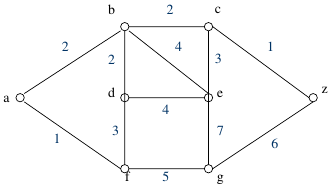
\includegraphics[width=0.55\textwidth]{d1}
\caption{Ejemplo inicial}
\end{figure}

Empezando desde el punto $a$, escogemos el camino que lleva al punto $f$, ya que es el camino de menor coste disponible, y lo metemos en el conjunto solución.

\begin{figure}[!h]
\centering
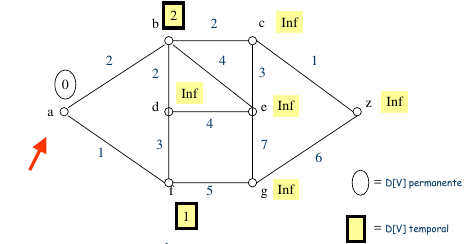
\includegraphics[width=0.7\textwidth]{d2}
\caption{Primera iteración}
\end{figure}

Ahora, el conjunto de vértices candidatos son $d$ y $g$. La distancia desde el punto, al ser mayor la distancia que recorremos hasta cualquiera de los dos puntos, cambiamos el conjunto solución y cogemos el punto $b$.

\begin{figure}[!h]
\centering
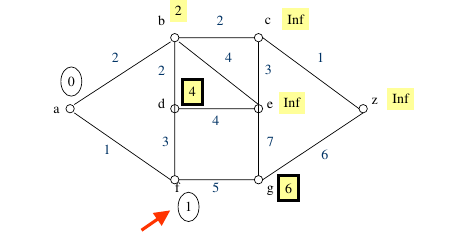
\includegraphics[width=0.7\textwidth]{d3}
\caption{Segunda iteración}
\end{figure}

\newpage

A continuación, salen tres nuevos posibles candidatos: $c$, $d$ y $e$, de los cuales, el que meteremos en el conjunto solución será el vértice $c$ por ser un camino mínimo.

\begin{figure}[!h]
\centering
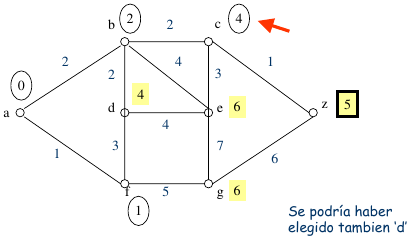
\includegraphics[width=0.7\textwidth]{d4}
\caption{Tercera iteración}
\end{figure}

En este caso, el vértice $d$ estaría en el conjunto solución, y al analizar los posibles caminos mínimos, sería desechado por no formar un camino mínimo, volviendo al estado de la iteración anterior.

\begin{figure}[!h]
\centering
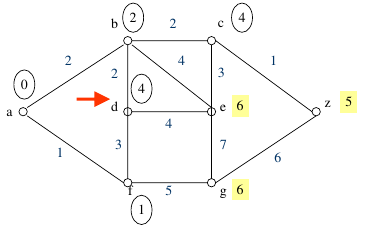
\includegraphics[width=0.7\textwidth]{d5}
\caption{Iteración que saldría de coger el vértice $d$}
\end{figure}

En este estado, los vértices candidatos al conjunto solución son el vértice $z$ y el vértice $e$. Como $z$ forma camino mínimo con $c$, lo metemos en el conjunto solución. Como además es nuestro destino, terminamos el algoritmo proporcionando la solución con el camino mínimo de longitud $5 \rightarrow $ $A-B-C-Z$

\begin{figure}[!h]
\centering
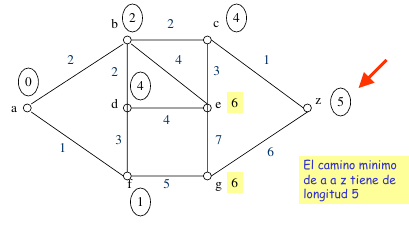
\includegraphics[width=0.7\textwidth]{d6}
\caption{asdfsa}
\end{figure}

\end{center}

\newpage

\subsubsection{\textcolor{electriccrimson}Análisis de Eficiencia}

El análisis de este algoritmo es parecido al del algoritmo de \hyperref[algprim]{Prim}, del cual se deduce que el algoritmo pertenece al orden de $O(A \log V)$. Aunque realmente, su eficiencia pertenece a $O((A+V)\log V)$, pero se supone que $A$ es mucho mayor que $V$. Además, si el grafo fuera muy denso, $A~\approx~V$


\section{\textcolor{electriccrimson}Heurística Greedy}

Ante los problemas NP-Completos, la solución exacta puede requerir órdenes factoriales o exponenciales (el problema de la \textit{explosión combinatoria}), por lo que nos llevaría mucho tiempo y recursos obtener esa solución o directamente es imposible de calcular. 

El objetivo es obtener ``buenas'' soluciones en un tiempo de ejecución \textbf{\textit{\textcolor{electriccrimson}{razonable}}}. Para ello, usaremos un tipo de algoritmos conocidos como \textbf{\textcolor{electriccrimson}{algoritmos de aproximación}}, que garantizan una solución más o menos buena, o una cierta aproximación respecto al óptimo.

Un tipo de estos algoritmos son las \textbf{\textcolor{electriccrimson}{heurísticas greedy}}. Son algoritmos basados en el conocimiento ``intuitivo'' o ``experto'' del programador sobre determinado problema, que nos proporcionará soluciones más o menos buenas, donde la clave de estas soluciones está en diseñar buenas funciones de selección. 

Para resumir, un algoritmo que produzca soluciones exactas o muy aproximadas (\hyperref[backtracking]{Backtracking} o \hyperref[branchandbound]{Branch\&Bound}) será mucho más lento y consumirá más recursos que un algoritmo que haga una aproximación de menor calidad y tarde mucho menos como pueden ser los algoritmos Greedy.

Un buen ejemplo de uso es el problema del \textbf{\textcolor{electriccrimson}viajante de comercio}.

\subsection{\textcolor{electriccrimson}El problema del viajante de comercio}

Dado un grafo no dirigido, completo y ponderado $G=(V,A)$, encontrar un ciclo de coste mínimo que pase por todos los nodos.

Este es un problema de optimización de tipo \textbf{NP-Completo}, del que necesitamos obtener una solución eficiente.

Para resolver este problema podemos usar un enfoque greedy, en el cual podemos tomar como candidatos:

\begin{description}
    \item [Nodos]: Se empieza desde un nodo cualquiera y las siguientes iteraciones sería moverse a los nodos no visitados más cercanos.

    \item [Aristas]: Imitar el algoritmo de \hyperref[kruskal]{Kruskal}, pero haciendo que se forme un ciclo.
\end{description}

Partiendo de un ejemplo como el siguiente, en el que tomamos los nodos como candidatos:

\begin{center}
    \input{heuristicasGre.latex}
    \\Partiendo del nodo que está en azul
\end{center}

En este ejemplo obtenemos la siguiente solución $(5,1,2,3,4)$ y coste total: $45+10+20+15+50=140)$

\begin{center}
    \input{heuristicasGre1.latex}
    \\Partiendo del nodo que está en azul
\end{center}

Y en este segundo ejemplo, obtenemos un camino solución $(5,3,4,2,1)$ y coste total: $30+15+25+10+45=15$.

Y en el caso de que cogieramos las aristas, la solución es $((1,2),(4,3),(2,3),(1,5),(4,5))$ con un coste total $= 10+15+20+45+50=140$.

Con esto podemos concluir que no son algoritmos óptimos sino que aportan una solución ``buena'', cercana a la óptima, y que ambos enfoques dan resultados similares.

\subsection{\textcolor{electriccrimson}El problema del coloreo de un grafo}

Dado un grafo plano $G=(V,E)$, determinar el mínimo número de colores que se necesitan para colorear todos sus vértices, y que no haya dos de ellos adyacentes pintados con el mismo color. 

Si el grafo no fuera plano, el número de colores necesario puede ser igual al número de vértices que tenga.

Este problema tiene una gran cantidad de aplicaciones, como pueden ser la representación de mapas, diseño de páginas webs, diseño de carreteras...

Este tipo de problema es un problema NP, que puede ser resuelto por un algoritmo Greedy, ya que reúne todas las características necesarias. Para ello usaremos el \textbf{\textcolor{electriccrimson}{teorema de Appel-Hanke}}, el cual dice que todo grafo plano, como mucho necesitará 4 colores diferentes para pintar sus nodos de modo que no haya vértices adyacentes con el mismo color.

En este caso, usaremos una \textbf{\textcolor{electriccrimson}{heurística Greedy}} para obtener una solución, partiendo de los siguiente:

\begin{enumerate}[---]
    \item Al principio no tenemos ningún nodo coloreado.
    \item Se escoge un color $colorActual=1$.
    \item Para cada uno de los nodos sin colorear (función \textit(selección)):
    \begin{enumerate}[$\bullet$]
        \item Comprobar si se le puede asignar el color actual (\textit{Factible(X)}.
        \item Si se puede, se asigna. En caso contrario, no se colorea.
    \end{enumerate}
    \item Si quedan nodos sin colorear, se escoge otro color ($colorActual:=colorActual+1$) y retomamos el paso anterior.
\end{enumerate}

\subsubsection{\textcolor{electriccrimson}Implementación del algoritmo}

\begin{minted}[linenos]{pascal}
function Coloreo(G(V,A):Grafo)
    nuevoColor:=null
    for v in G.verticesNoColoreados() do:
        if v.noAdyacente(nuevoColor) then:
            v.colorear();
            nuevoColor.add(v);
        end
    end
end    
\end{minted}

Este algoritmo proporciona soluciones en tiempos pertenecientes a $O(n)$, pero no siempre da la solución óptima.

\chapter{\textcolor{amethyst}Programación Dinámica}

\section{\textcolor{amethyst}Introducción}

La técnica de programación dinámica se puede considerar una versión secuencial de los problemas Divide y Vencerás. Esto es debido a que resuelve problemas formados por otros subproblemas, al igual que los problemas Divide y Vencerás, pero a diferencia de éstos, evita resolver lo mismo más de una vez.

Por ejemplo, al resolver la sucesión de Fibonacci 

\begin{displaymath}
    f_n = \left\{ \begin{array}{ll}
n & \qquad \textrm{si $n = 0$, $n = 1$}\\
f_{n-1} + f_{n-2} & \qquad \textrm{en otro caso} \\
\end{array} \right.
\end{displaymath}


mediante Divide y vencerás se genera el siguiente árbol:

\begin{center}
\input{fib.latex}
\end{center}

Como se puede apreciar, se repiten varios cálculos como el de $F(n-2)$ o el de $F(n-3)$. Esto en Programación Dinámica se evita mediante el uso de \textit{\textcolor{amethyst}{tablas}}: cada valor calculado se guarda en una tabla, así, sólo hay que calcularlo la primera vez y el resto, simplemente basta con consultar la tabla. Esto se conoce como \textit{\textcolor{amethyst}{solapamiento de subproblemas}}.

\label{ascendentes}
Los algoritmos Divide y Vencerás se conocen como \textit{\textcolor{amethyst}{Métodos descendentes}} porque empiezan con el problema original y lo van descomponiendo en problemas más pequeños hasta llegar al caso base. En cambio, los algoritmos basados en Programación Dinámica se conocen como \textit{\textcolor{amethyst}{Métodos ascendentes}} ya que empiezan resolviendo los casos base, guardando las soluciones en una tabla y combinándolas para llegar al problema original.

\section{\textcolor{amethyst}Elementos de la programación dinámica}
Para aplicar un algoritmo de Programación Dinámica hay que seguir los siguientes casos:
\begin{enumerate}
    \item Obtener una \textit{\textcolor{amethyst}{descomposición recurrente}} del problema, formada por una ecuación recurrente y unos casos base. Al igual que en Divide y vencerás.
    \item Definir la \textit{\textcolor{amethyst}{estrategia}} de aplicación de la fórmula: tipo de tablas a usar y forma de rellenarlas.
    \item Especificar cómo se \textit{\textcolor{amethyst}{recompone la solución}} final a partir de los valores de las tablas.
\end{enumerate}

Para poder hacer una descomposición recurrente del problema, lo mejor es verlo como un \textit{\textcolor{amethyst}{proceso de toma de decisiones}}. Por ejemplo, en el ejemplo de la \textit{\textcolor{amethyst}{Mochila 0/1}}, la decisión está en coger o no coger un objeto y de ahí sacamos la ecuación recurrente:

\begin{equation*}
Mochila(k,m) = 
\begin{cases}
0 & \text{si } k = 0 \text{ ó } m = 0,\\
-\infty & \text{si } k<0 \text{ ó } m<0\\
max\{Mochila(k-1,m), b_k + Mochila(k-1,m-p_k)\}
\end{cases} 
\end{equation*}


Como dijimos antes, para no repetir cálculos, en Programación Dinámica se usan \textit{\textcolor{amethyst}{tablas}} para almacenar resultados parciales. La parte mala de esto es que nos podemos quedar sin memoria para almacenar la tabla si ésta crece demasiado.


\subsection{\textcolor{amethyst}Principio de optimalidad de Bellman}

Para que una solución sea óptima, cada una de las subsoluciones que la componen debe ser también óptimas.

Dado un problema $P$ con $n$ elementos, si la secuencia óptima es $e_1 e_2 \cdots e_k \cdots e_n$ entonces:
\begin{enumerate}[\color{amethyst}{$\heartsuit$}]
    \item $e_1 e_2 \cdots e_k$ es solución al problema $P$ considerando los $k$ primeros elementos.
    \item $e_{k+1} \cdots e_n$ es solución al problema $P$ considerando los elementos desde $k+1$ hasta $n$.
\end{enumerate}

El \textit{\textcolor{amethyst}{Principio de Optimalidad de Bellman}} dice así:

\begin{tabular}{p{12.5cm}}
\hline
``Una política óptima tiene la propiedad de que, sean cuales sea el estado inicial y la decisión inicial, las decisiones restantes deben constituir una solución óptima con respecto al estado resultante de la primera decisión.''\\
\hline
\end{tabular}

En informática, un problema que puede descomponerse de esta forma se dice que presenta subestructuras optimales.

El prinicipio de optimalidad \textbf{\textcolor{amethyst}{NO}} nos dice que, si tenemos soluciones óptimas a los subproblemas, podamos combinarlas para obtener la solución óptima del problema original.

Por ejemplo, en el problema de \textit{\textcolor{amethyst}{cambio de monedas}} tenemos que:
\begin{enumerate}[\color{amethyst}{$\heartsuit$}]
    \item La solución óptima para $7$ céntimos es $5+2$ céntimos.
    \item La solución óptima para $6$, $5+1$.
    \item Pero la solución para $13$ no es $(5+2) + (5+1)$ sino $(10+1+2)$.
\end{enumerate}

\subsection{\textcolor{amethyst}Definición recursiva de la solución óptima y Cálculo de la solución óptima}

Para aplicar programación dinámica debemos comprobar que se cumple el Principio de Optimalidad y definir recursivamente la solución óptima del problema.

Para calcular la solución óptima usando el \hyperref[ascendentes]{enfoque ascendente} tenemos que determinar el tamaño de la tabla (númerode subproblemas a resolver), identificar los casos base del problema e ir calculando los valores de las soluciones más complejas a partir de los casos base y las soluciones más simples.

A partir de los datos que obtenemos en la tabla, determinamos la solución óptima.

\section{\textcolor{amethyst}Ejemplos}

\subsection{\textcolor{amethyst}Multiplicación encadenada de matrices}

Tenemos cuatro matrices de las siguientes dimensiones: $A(13 \times 5)$, $B(5 \times 89)$, $C(89 \times 3)$ y $D(3 \times 34)$.

Para calcular su multiplicación podemos hacerlo de varias formas. La siguiente tabla refleja, para cada forma de multiplicar las matrices (el orden en el que hacemos cada multiplicación, es decir, donde ponemos cada paréntesis) el número de operaciones necesarias:

\begin{tabular}{l|r}
& num multip. \\
\hline
$(((AB)C)D)$ & $10582$ \\
$(AB)(CD)$ & $54201$ \\
$(A(BC))D$ & $2856$ \\
$A((BC)D)$ & $4055$ \\
$A(B(CD))$ & $26418$ \\
\end{tabular}

Como se ve, el orden es bastante importante pues nuestro programa podría ser 19 veces más rápido.

Para saber cuál es la mejor forma de poner los paréntesis, para cada forma de ponerlos calculamos el número de operaciones requeridas\footnote{Para multiplicar dos matrices de $p \times q$ y $q \times r$ dimensiones respectivamente, necesitamos $pqr$ multiplicaciones de escalares}.

Ahora bien, como la forma de colocar los paréntesis sube exponencialmente conforme más matrices para multiplicar hay, la forma ``directa'' de calcular el número de operaciones es inviable.

Aplicamos \textit{\textcolor{amethyst}{Programación Dinámica}}:

\begin{description}
    \item[Aplicación del principio de optimalidad]: Si el mejor modo de realizar el producto exige dividir las matrices entre la $i$ y la $i+1$ los productos
    \begin{displaymath}
        M_1 M_2 \cdots M_i ~ \textrm{y} ~ M_{i+1} M_{i+2} \cdots M_n
    \end{displaymath}

    deben ser realizados de forma óptima de forma que el total también sea óptimo.

    \item[Método]: Construimos la matriz $[m_{ij}]$ ($1 < i < j < n$) donde $m_{ij}$ da el óptimo para la parte $M_i M_i+1 \cdots M_j$ del producto total. La solución final vendrá dada por $m_{1n}$.

    \item[Construcción de la matriz]:
    \begin{enumerate}[\color{amethyst}{$\heartsuit$}]
        \item Guardamos las dimensiones de cada matriz del producto en un vector $d$ con $n$ componentes, de forma la matriz $M_i$ tiene dimensiones $d_{i-1} \times d_i$. 

        En el ejemplo anterior ($A(13 \times 5)$, $B(5 \times 89)$, $C(89 \times 3)$, $D(3 \times 34)$), este vector sería $d = (13,5,89,3,34)$.

        \item La diagonal $s$ de $[m_{ij}]$ contiene los $m_{ij}$ tales que $j-i=s$. Por tanto tendremos:

        \begin{equation*}
        m_{ij} = 
        \begin{cases}
        0 & \text{si } i = j,\\
        min\{m_{ik} + m_{k+1, j} + d_{i-1} d_k d_j\} & \text{si } i < j
        \end{cases} 
        \end{equation*}

        Es decir, siempre intentaremos quedarnos con la posibilidad que menos operaciones implique realizar.

        Para $s=1$:
        \begin{enumerate}[$\longrightarrow$]
            \item $m_{12} = 5785$
            \item $m_{23} = 1335$
            \item $m_{34} = 9078$
        \end{enumerate}

        Para $s=2$:
        \begin{enumerate}[$\longrightarrow$]
            \item $m_{13} = min(m_{11} + m_{23} + 13 \times 5 \times 3, m_{12} + m_{33} + 13 \times 89 \times 3) = min(1530, 9256) = 1530$
            \item $m_{24} = min(m_{22} + m_{34} + 5 \times 89 \times 34, m_{23} + m_{44} + 5 \times 3 \times 34) = min(24208, 1845) = 1845$
        \end{enumerate}

        Para $s=3$:
        \begin{enumerate}[$\longrightarrow$]
            \item         
                \begin{equation*}
                m_{14} = min(
                \begin{cases}
                \{k=1\} ~ m_{11} + m_{24} + 13 \times 5 \times 34, \\
                \{k=2\} ~ m_{12} + m_{34} + 13 \times 89 \times 34, \\
                \{k=3\} ~ m_{13} + m_{44} + 13 \times 3 \times 34)
                \end{cases}
                = min (4055, 54201, 2856) = 2856
                \end{equation*}
        \end{enumerate}
    \end{enumerate}

    En resumen, nuestra tabla sería la siguiente:

    \begin{tabular}{c | c c c c l}
    & $j=1$ & $2$ & $3$ & $4$ & \\
    \cline{1-5}
    % \cmidrule{1-5} 
    % blackslashbox
    $i = 1$ &\textcolor{armygreen}{0} & \textcolor{azure}{5785} & \textcolor{coquelicot}{1530} & \textcolor{electricgreen}{2856} & \\
    $2$ & & \textcolor{armygreen}{0} & \textcolor{azure}{1335} & \textcolor{coquelicot}{1845} &  \textcolor{electricgreen}{$s=3$} \\
    $3$ & & & \textcolor{armygreen}{0} & \textcolor{azure}{9078} &  \textcolor{coquelicot}{$s=2$} \\
    4 & & & & \textcolor{armygreen}{0} &  \textcolor{azure}{$s=1$} \\
    & & & & & \textcolor{armygreen}{$s=0$} \\
    \end{tabular}
\end{description}

\subsection{\textcolor{amethyst}Distancia de edición}

Encontrar el mínimo de cambios que hay qué hacer y explicar cuáles son dichos cambios para las siguientes palabras:
\begin{enumerate}[a)]
    \item Vidas y Concurrentes
    \item Fácil y Difícil
    \item Meilenstein y Levenshtein
\end{enumerate}

Aplicando esta fórmula:
\begin{equation*}
    d(i,j) = 
    \begin{cases}
        d(i-1,j-1) & \textrm{si $s[i] = t[j]$} \\
        1 + min\{ d(i-1,j), d(i,j-1), d(i-1,j-1) \} & \textrm{si $s[i] \neq t[j]$}
    \end{cases}
\end{equation*}

donde:
\begin{enumerate}[$\bullet$]
    \item Mismo carácter: $d(i-1,j-1)$
    \item Inserción: $1 + d(i-1,j)$
    \item Borrado: $1 + d(i,j-1)$
    \item Modificación: $1 + d(i-1,j-1)$
\end{enumerate}

Para calcular un carácter $c[i][j]$ necesitamos los caracteres $c[i-1][j]$, $c[i][j-1]$ y $c[i-1][j-1]$ para elegir el mínimo de dichos caracteres. 

De una manera más gráfica, para calcular la casilla en blanco necesitamos las que están en negro:

\begin{center}
\begin{tabular}{|c|c|}
\hline
\rowcolor{Black} &  \\
\hline
\cellcolor{Black} & \\
\hline
\end{tabular}
\end{center}

\subsection{\textcolor{amethyst}Concurrentes - \textcolor{amethyst}Vidas}
\begin{center}
\begin{tabular}{c|c|c|c|c|c|c|}
\multicolumn{2}{r}{} & \multicolumn{1}{c}{V} & \multicolumn{1}{c}{I} & \multicolumn{1}{c}{D} & \multicolumn{1}{c}{A} & \multicolumn{1}{c}{S} \\ 
\cline{2-7} 
& $0$ & 1 & 2 & 3 & 4 & 5 \\
\cline{2-7} 
C & 1 & 1 & 2 & 3 & 4 & 5 \\
\cline{2-7}
O & 2 & 2 & 2 & 3 & 4 & 5 \\
\cline{2-7} 
N & 3 & 3 & 3 & 3 & 4 & 5 \\
\cline{2-7} 
C & 4 & 4 & 4 & 4 & 4 & 5 \\
\cline{2-7} 
U & 5 & 5 & 5 & 5 & 5 & 5 \\
\cline{2-7} 
R & 6 & 6 & 6 & 6 & 6 & 6 \\
\cline{2-7} 
R & 7 & 7 & 7 & 7 & 7 & 7 \\
\cline{2-7} 
E & 8 & 8 & 8 & 8 & 8 & 8 \\
\cline{2-7} 
N & 9 & 9 & 9 & 9 & 9 & 9 \\
\cline{2-7} 
T & 10 & 10 & 10 & 10 & 10 & 10 \\
\cline{2-7} 
E & 11 & 11 & 11 & 11 & 11 & 11 \\
\cline{2-7} 
S & 12 & 12 & 12 & 12 & 12 & \cellcolor{Green}11 \\
\cline{2-7}
\end{tabular}
\end{center}

Es decir, para pasar de Vidas a Concurrentes, el número mínimo de operaciones es 11. Estas operaciones son:

\begin{enumerate}
    \item La $S$ no se cambia pues coincide en ambas palabras por tanto no se toca.
    \begin{center}
\begin{tabular}{c|c|c|c|c|c|c|}
\multicolumn{2}{r}{} & \multicolumn{1}{c}{V} & \multicolumn{1}{c}{I} & \multicolumn{1}{c}{D} & \multicolumn{1}{c}{A} & \multicolumn{1}{c}{\textcolor{Red}{S}} \\ 
\cline{2-7} 
& $0$ & 1 & 2 & 3 & 4 & 5 \\
\cline{2-7} 
C & 1 & 1 & 2 & 3 & 4 & 5 \\
\cline{2-7}
O & 2 & 2 & 2 & 3 & 4 & 5 \\
\cline{2-7} 
N & 3 & 3 & 3 & 3 & 4 & 5 \\
\cline{2-7} 
C & 4 & 4 & 4 & 4 & 4 & 5 \\
\cline{2-7} 
U & 5 & 5 & 5 & 5 & 5 & 5 \\
\cline{2-7} 
R & 6 & 6 & 6 & 6 & 6 & 6 \\
\cline{2-7} 
R & 7 & 7 & 7 & 7 & 7 & 7 \\
\cline{2-7} 
E & 8 & 8 & 8 & 8 & 8 & 8 \\
\cline{2-7} 
N & 9 & 9 & 9 & 9 & 9 & 9 \\
\cline{2-7} 
T & 10 & 10 & 10 & 10 & 10 & 10 \\
\cline{2-7} 
E & 11 & 11 & 11 & 11 & \cellcolor{Cyan}{11} & 11 \\
\cline{2-7} 
\textcolor{Red}{S} & 12 & 12 & 12 & 12 & 12 & \cellcolor{Green}\textcolor{Red}{11} \\
\cline{2-7}
\end{tabular}
\end{center}

\item Como la $A$ y la $E$ no coinciden, cambiamos la $A$ por la $E$:
\begin{center}
\begin{tabular}{c|c|c|c|c|c|c|}
\multicolumn{2}{r}{} & \multicolumn{1}{c}{V} & \multicolumn{1}{c}{I} & \multicolumn{1}{c}{D} & \multicolumn{1}{c}{\textcolor{Red}{A}} & \multicolumn{1}{c}{S} \\ 
\cline{2-7} 
& $0$ & 1 & 2 & 3 & 4 & 5 \\
\cline{2-7} 
C & 1 & 1 & 2 & 3 & 4 & 5 \\
\cline{2-7}
O & 2 & 2 & 2 & 3 & 4 & 5 \\
\cline{2-7} 
N & 3 & 3 & 3 & 3 & 4 & 5 \\
\cline{2-7} 
C & 4 & 4 & 4 & 4 & 4 & 5 \\
\cline{2-7} 
U & 5 & 5 & 5 & 5 & 5 & 5 \\
\cline{2-7} 
R & 6 & 6 & 6 & 6 & 6 & 6 \\
\cline{2-7} 
R & 7 & 7 & 7 & 7 & 7 & 7 \\
\cline{2-7} 
E & 8 & 8 & 8 & 8 & 8 & 8 \\
\cline{2-7} 
N & 9 & 9 & 9 & 9 & 9 & 9 \\
\cline{2-7} 
T & 10 & 10 & 10 & \cellcolor{Cyan}{10} & 10 & 10 \\
\cline{2-7} 
\textcolor{Red}{E} & 11 & 11 & 11 & 11 & \textcolor{Red}{11} & 11 \\
\cline{2-7} 
S & 12 & 12 & 12 & 12 & 12 & \cellcolor{Green}11 \\
\cline{2-7}
\end{tabular}
\end{center}

\item Como la $D$ y la $T$ no coinciden, sustituimos la $D$ por la $T$:
\begin{center}
\begin{tabular}{c|c|c|c|c|c|c|}
\multicolumn{2}{r}{} & \multicolumn{1}{c}{V} & \multicolumn{1}{c}{I} & \multicolumn{1}{c}{\textcolor{Red}{D}} & \multicolumn{1}{c}{A} & \multicolumn{1}{c}{S} \\ 
\cline{2-7} 
& $0$ & 1 & 2 & 3 & 4 & 5 \\
\cline{2-7} 
C & 1 & 1 & 2 & 3 & 4 & 5 \\
\cline{2-7}
O & 2 & 2 & 2 & 3 & 4 & 5 \\
\cline{2-7} 
N & 3 & 3 & 3 & 3 & 4 & 5 \\
\cline{2-7} 
C & 4 & 4 & 4 & 4 & 4 & 5 \\
\cline{2-7} 
U & 5 & 5 & 5 & 5 & 5 & 5 \\
\cline{2-7} 
R & 6 & 6 & 6 & 6 & 6 & 6 \\
\cline{2-7} 
R & 7 & 7 & 7 & 7 & 7 & 7 \\
\cline{2-7} 
E & 8 & 8 & 8 & 8 & 8 & 8 \\
\cline{2-7} 
N & 9 & 9 & \cellcolor{Cyan}{9} & 9 & 9 & 9 \\
\cline{2-7} 
\textcolor{Red}{T} & 10 & 10 & 10 & \textcolor{Red}{10} & 10 & 10 \\
\cline{2-7} 
E & 11 & 11 & 11 & 11 & \cellcolor{Green}{11} & 11 \\
\cline{2-7} 
S & 12 & 12 & 12 & 12 & 12 & \cellcolor{Green}11 \\
\cline{2-7}
\end{tabular}
\end{center}

\item Procedemos de igual manera hasta llegar a la $E$ y la $V$:

\begin{center}
\begin{tabular}{c|c|c|c|c|c|c|}
\multicolumn{2}{r}{} & \multicolumn{1}{c}{\textcolor{Red}{V}} & \multicolumn{1}{c}{\textcolor{Red}{I}} & \multicolumn{1}{c}{D} & \multicolumn{1}{c}{A} & \multicolumn{1}{c}{S} \\ 
\cline{2-7} 
& $0$ & 1 & 2 & 3 & 4 & 5 \\
\cline{2-7} 
C & 1 & 1 & 2 & 3 & 4 & 5 \\
\cline{2-7}
O & 2 & 2 & 2 & 3 & 4 & 5 \\
\cline{2-7} 
N & 3 & 3 & 3 & 3 & 4 & 5 \\
\cline{2-7} 
C & 4 & 4 & 4 & 4 & 4 & 5 \\
\cline{2-7} 
U & 5 & 5 & 5 & 5 & 5 & 5 \\
\cline{2-7} 
R & 6 & 6 & 6 & 6 & 6 & 6 \\
\cline{2-7} 
R & 7 & \cellcolor{Cyan}7 & 7 & 7 & 7 & 7 \\
\cline{2-7} 
\textcolor{Red}{E} & 8 & \cellcolor{Green}{8} & 8 & 8 & 8 & 8 \\
\cline{2-7} 
\textcolor{Red}{N} & 9 & 9 & \cellcolor{Green}{9} & 9 & 9 & 9 \\
\cline{2-7} 
T & 10 & 10 & 10 & \cellcolor{Green}{10} & 10 & 10 \\
\cline{2-7} 
E & 11 & 11 & 11 & 11 & \cellcolor{Green}{11} & 11 \\
\cline{2-7} 
S & 12 & 12 & 12 & 12 & 12 & \cellcolor{Green}11 \\
\cline{2-7}
\end{tabular}
\end{center}

\item Insertamos el resto de caracteres: $R$, $R$, $U$, $C$, $N$, $O$ y $C$
\begin{center}
\begin{tabular}{c|c|c|c|c|c|c|}
\multicolumn{2}{r}{} & \multicolumn{1}{c}{V} & \multicolumn{1}{c}{I} & \multicolumn{1}{c}{D} & \multicolumn{1}{c}{A} & \multicolumn{1}{c}{S} \\ 
\cline{2-7} 
& $0$ & 1 & 2 & 3 & 4 & 5 \\
\cline{2-7} 
\textcolor{Red}{C} & 1 & \cellcolor{Green}1 & 2 & 3 & 4 & 5 \\
\cline{2-7}
\textcolor{Red}{O} & 2 & \cellcolor{Green}2 & 2 & 3 & 4 & 5 \\
\cline{2-7} 
\textcolor{Red}{N} & 3 & \cellcolor{Green}3 & 3 & 3 & 4 & 5 \\
\cline{2-7} 
\textcolor{Red}{C} & 4 & \cellcolor{Green}4 & 4 & 4 & 4 & 5 \\
\cline{2-7} 
\textcolor{Red}{U} & 5 & \cellcolor{Green}5 & 5 & 5 & 5 & 5 \\
\cline{2-7} 
\textcolor{Red}{R} & 6 & \cellcolor{Green}6 & 6 & 6 & 6 & 6 \\
\cline{2-7} 
\textcolor{Red}{R} & 7 & \cellcolor{Green}7 & 7 & 7 & 7 & 7 \\
\cline{2-7} 
E & 8 & \cellcolor{Green}{8} & 8 & 8 & 8 & 8 \\
\cline{2-7} 
N & 9 & 9 & \cellcolor{Green}{9} & 9 & 9 & 9 \\
\cline{2-7} 
T & 10 & 10 & 10 & \cellcolor{Green}{10} & 10 & 10 \\
\cline{2-7} 
E & 11 & 11 & 11 & 11 & \cellcolor{Green}{11} & 11 \\
\cline{2-7} 
S & 12 & 12 & 12 & 12 & 12 & \cellcolor{Green}11 \\
\cline{2-7}
\end{tabular}
\end{center}
\end{enumerate}

\newpage
\subsection{\textcolor{amethyst}Difícil - \textcolor{amethyst}Fácil}
No tenemos en cuenta si un carácter está acentuado o no.
\begin{center}
\begin{tabular}{c|c|c|c|c|c|c|}
\multicolumn{2}{r}{} & \multicolumn{1}{c}{F} & \multicolumn{1}{c}{Á} & \multicolumn{1}{c}{C} & \multicolumn{1}{c}{I} & \multicolumn{1}{c}{L} \\ 
\cline{2-7} 
 & 0 & 1 & 2 & 3 & 4 & 5 \\
\cline{2-7}
D & 1 & 1 & 2 & 3 & 4 & 5 \\
\cline{2-7} 
I & 2 & 2 & 2 & 3 & 3 & 4 \\
\cline{2-7} 
F & 3 & 2 & 3 & 3 & 4 & 4 \\
\cline{2-7} 
Í & 4 & 3 & 3 & 4 & 3 & 4 \\
\cline{2-7} 
C & 5 & 4 & 4 & 3 & 4 & 4 \\
\cline{2-7} 
I & 6 & 5 & 5 & 4 & 3 & 4 \\
\cline{2-7} 
L & 7 & 6 & 6 & 5 & 4 & \cellcolor{Green}3 \\
\cline{2-7}  
\end{tabular}
\end{center}

Por tanto, para pasar de Fácil a Difícil, el número mínimo de operaciones es 3. Estas operaciones son:

\begin{enumerate}
    \item La $L$, la $I$ y la $C$ no cambian, pues coinciden en ambas palabras:
\begin{center}
\begin{tabular}{c|c|c|c|c|c|c|}
\multicolumn{2}{r}{} & \multicolumn{1}{c}{F} & \multicolumn{1}{c}{Á} & \multicolumn{1}{c}{\textcolor{Red}{C}} & \multicolumn{1}{c}{\textcolor{Red}{I}} & \multicolumn{1}{c}{\textcolor{Red}{L}} \\ 
\cline{2-7} 
 & 0 & 1 & 2 & 3 & 4 & 5 \\
\cline{2-7}
D & 1 & 1 & 2 & 3 & 4 & 5 \\
\cline{2-7} 
I & 2 & 2 & 2 & 3 & 3 & 4 \\
\cline{2-7} 
F & 3 & 2 & 3 & 3 & 4 & 4 \\
\cline{2-7} 
Í & 4 & 3 & 3 & 4 & 3 & 4 \\
\cline{2-7} 
\textcolor{Red}{C} & 5 & 4 & 4 & \cellcolor{Green}3 & 4 & 4 \\
\cline{2-7} 
\textcolor{Red}{I} & 6 & 5 & 5 & 4 & \cellcolor{Green}3 & 4 \\
\cline{2-7} 
\textcolor{Red}{L} & 7 & 6 & 6 & 5 & 4 & \cellcolor{Green}3 \\
\cline{2-7}  
\end{tabular}
\end{center}

\item Modificamos la $A$ por la $I$:
\begin{center}
\begin{tabular}{c|c|c|c|c|c|c|}
\multicolumn{2}{r}{} & \multicolumn{1}{c}{F} & \multicolumn{1}{c}{\textcolor{Red}{A}} & \multicolumn{1}{c}{C} & \multicolumn{1}{c}{I} & \multicolumn{1}{c}{L} \\ 
\cline{2-7} 
 & 0 & 1 & 2 & 3 & 4 & 5 \\
\cline{2-7}
D & 1 & 1 & 2 & 3 & 4 & 5 \\
\cline{2-7} 
I & 2 & 2 & 2 & 3 & 3 & 4 \\
\cline{2-7} 
F & 3 & \cellcolor{Cyan}2 & 3 & 3 & 4 & 4 \\
\cline{2-7} 
\textcolor{Red}{I} & 4 & 3 & \textcolor{Red}{3} & 4 & 3 & 4 \\
\cline{2-7} 
C & 5 & 4 & 4 & \cellcolor{Green}3 & 4 & 4 \\
\cline{2-7} 
I & 6 & 5 & 5 & 4 & \cellcolor{Green}3 & 4 \\
\cline{2-7} 
L & 7 & 6 & 6 & 5 & 4 & \cellcolor{Green}3 \\
\cline{2-7}  
\end{tabular}
\end{center}

\item La $F$ permanece igual pues coincide en ambas palabras:
\begin{center}
\begin{tabular}{c|c|c|c|c|c|c|}
\multicolumn{2}{r}{} & \multicolumn{1}{c}{\textcolor{Red}{F}} & \multicolumn{1}{c}{A} & \multicolumn{1}{c}{C} & \multicolumn{1}{c}{I} & \multicolumn{1}{c}{L} \\ 
\cline{2-7} 
 & 0 & 1 & 2 & 3 & 4 & 5 \\
\cline{2-7}
D & 1 & 1 & 2 & 3 & 4 & 5 \\
\cline{2-7} 
I & \cellcolor{Cyan}2 & 2 & 2 & 3 & 3 & 4 \\
\cline{2-7} 
\textcolor{Red}{F} & 3 & \textcolor{Red}{2} & 3 & 3 & 4 & 4 \\
\cline{2-7} 
I & 4 & 3 & \cellcolor{Green}3 & 4 & 3 & 4 \\
\cline{2-7} 
C & 5 & 4 & 4 & \cellcolor{Green}3 & 4 & 4 \\
\cline{2-7} 
I & 6 & 5 & 5 & 4 & \cellcolor{Green}3 & 4 \\
\cline{2-7} 
L & 7 & 6 & 6 & 5 & 4 & \cellcolor{Green}3 \\
\cline{2-7}  
\end{tabular}
\end{center}

\item Y por último, insertamos la $D$ y la $I$:
\begin{center}
\begin{tabular}{c|c|c|c|c|c|c|}
\multicolumn{2}{r}{} & \multicolumn{1}{c}{F} & \multicolumn{1}{c}{A} & \multicolumn{1}{c}{C} & \multicolumn{1}{c}{I} & \multicolumn{1}{c}{L} \\ 
\cline{2-7} 
 & 0 & 1 & 2 & 3 & 4 & 5 \\
\cline{2-7}
\textcolor{Red}{D} & \cellcolor{Green}1 & 1 & 2 & 3 & 4 & 5 \\
\cline{2-7} 
\textcolor{Red}{I} & \cellcolor{Green}2 & 2 & 2 & 3 & 3 & 4 \\
\cline{2-7} 
F & 3 & \cellcolor{Green}2 & 3 & 3 & 4 & 4 \\
\cline{2-7} 
I & 4 & 3 & \cellcolor{Green}3 & 4 & 3 & 4 \\
\cline{2-7} 
C & 5 & 4 & 4 & \cellcolor{Green}3 & 4 & 4 \\
\cline{2-7} 
I & 6 & 5 & 5 & 4 & \cellcolor{Green}3 & 4 \\
\cline{2-7} 
L & 7 & 6 & 6 & 5 & 4 & \cellcolor{Green}3 \\
\cline{2-7}  
\end{tabular}
\end{center}
\end{enumerate}

\subsection{\textcolor{amethyst}Levenshtein - \textcolor{amethyst}Meilenstein}
\begin{center}
\begin{tabular}{c|c|c|c|c|c|c|c|c|c|c|c|c|}
\multicolumn{2}{r}{} & \multicolumn{1}{c}{M} & \multicolumn{1}{c}{E} & \multicolumn{1}{c}{I} & \multicolumn{1}{c}{L} & \multicolumn{1}{c}{E} & \multicolumn{1}{c}{N} & \multicolumn{1}{c}{S} & \multicolumn{1}{c}{T} & \multicolumn{1}{c}{E} & \multicolumn{1}{c}{I} & \multicolumn{1}{c}{N} \\ 
\cline{2-13} 
& 0 & 1 & 2 & 3 & 4 & 5 & 6 & 7 & 8 & 9 & 10 & 11 \\
\cline{2-13}
L & 1 & 1 & 2 & 3 & 3 & 4 & 5 & 6 & 7 & 8 & 9 & 10 \\
\cline{2-13} 
E & 2 & 2 & 1 & 2 & 3 & 3 & 4 & 5 & 6 & 7 & 8 & 9 \\
\cline{2-13} 
V & 3 & 3 & 2 & 2 & 3 & 4 & 4 & 5 & 6 & 7 & 8 & 9 \\
\cline{2-13} 
E & 4 & 4 & 3 & 3 & 3 & 3 & 4 & 5 & 6 & 6 & 7 & 8 \\
\cline{2-13} 
N & 5 & 5 & 4 & 4 & 4 & 4 & 3 & 4 & 5 & 6 & 7 & 7 \\
\cline{2-13} 
S & 6 & 6 & 5 & 5 & 5 & 5 & 4 & 3 & 4 & 5 & 6 & 7 \\
\cline{2-13} 
H & 7 & 7 & 6 & 6 & 6 & 6 & 5 & 4 & 4 & 5 & 6 & 7 \\
\cline{2-13} 
T & 8 & 8 & 7 & 7 & 7 & 7 & 6 & 5 & 4 & 5 & 6 & 7 \\
\cline{2-13}
E & 9 & 9 & 8 & 8 & 8 & 7 & 7 & 6 & 5 & 4 & 5 & 6 \\
\cline{2-13} 
I & 10 & 10 & 9 & 8 & 9 & 8 & 8 & 7 & 6 & 5 & 4 & 5 \\
\cline{2-13} 
N & 11 & 11 & 10 & 9 & 9 & 9 & 8 & 8 & 7 & 6 & 5 & \cellcolor{Green}4 \\
\cline{2-13} 
\end{tabular}
\end{center}

Por tanto, necesitamos hacer 4 cambios como mínimo para pasar de Meilenstein a Levenshtein. Estos cambios serían:

\begin{enumerate}
    \item Los cuatro últimos caracteres de ambas palabras coinciden, por tanto, no se cambian:
\begin{center}
\begin{tabular}{c|c|c|c|c|c|c|c|c|c|c|c|c|}
\multicolumn{2}{r}{} & \multicolumn{1}{c}{M} & \multicolumn{1}{c}{E} & \multicolumn{1}{c}{I} & \multicolumn{1}{c}{L} & \multicolumn{1}{c}{E} & \multicolumn{1}{c}{N} & \multicolumn{1}{c}{S} & \multicolumn{1}{c}{\textcolor{Red}{T}} & \multicolumn{1}{c}{\textcolor{Red}{E}} & \multicolumn{1}{c}{\textcolor{Red}{I}} & \multicolumn{1}{c}{\textcolor{Red}{N}} \\ 
\cline{2-13} 
& 0 & 1 & 2 & 3 & 4 & 5 & 6 & 7 & 8 & 9 & 10 & 11 \\
\cline{2-13}
L & 1 & 1 & 2 & 3 & 3 & 4 & 5 & 6 & 7 & 8 & 9 & 10 \\
\cline{2-13} 
E & 2 & 2 & 1 & 2 & 3 & 3 & 4 & 5 & 6 & 7 & 8 & 9 \\
\cline{2-13} 
V & 3 & 3 & 2 & 2 & 3 & 4 & 4 & 5 & 6 & 7 & 8 & 9 \\
\cline{2-13} 
E & 4 & 4 & 3 & 3 & 3 & 3 & 4 & 5 & 6 & 6 & 7 & 8 \\
\cline{2-13} 
N & 5 & 5 & 4 & 4 & 4 & 4 & 3 & 4 & 5 & 6 & 7 & 7 \\
\cline{2-13} 
S & 6 & 6 & 5 & 5 & 5 & 5 & 4 & 3 & 4 & 5 & 6 & 7 \\
\cline{2-13} 
H & 7 & 7 & 6 & 6 & 6 & 6 & 5 & 4 & 4 & 5 & 6 & 7 \\
\cline{2-13} 
\textcolor{Red}{T} & 8 & 8 & 7 & 7 & 7 & 7 & 6 & 5 & \cellcolor{Green}4 & 5 & 6 & 7 \\
\cline{2-13}
\textcolor{Red}{E} & 9 & 9 & 8 & 8 & 8 & 7 & 7 & 6 & 5 & \cellcolor{Green}4 & 5 & 6 \\
\cline{2-13} 
\textcolor{Red}{I} & 10 & 10 & 9 & 8 & 9 & 8 & 8 & 7 & 6 & 5 & \cellcolor{Green}4 & 5 \\
\cline{2-13} 
\textcolor{Red}{N} & 11 & 11 & 10 & 9 & 9 & 9 & 8 & 8 & 7 & 6 & 5 & \cellcolor{Green}4 \\
\cline{2-13} 
\end{tabular}
\end{center}

\item Insertamos la $H$:
\begin{center}
\begin{tabular}{c|c|c|c|c|c|c|c|c|c|c|c|c|}
\multicolumn{2}{r}{} & \multicolumn{1}{c}{M} & \multicolumn{1}{c}{E} & \multicolumn{1}{c}{I} & \multicolumn{1}{c}{L} & \multicolumn{1}{c}{E} & \multicolumn{1}{c}{N} & \multicolumn{1}{c}{S} & \multicolumn{1}{c}{T} & \multicolumn{1}{c}{E} & \multicolumn{1}{c}{I} & \multicolumn{1}{c}{N} \\ 
\cline{2-13} 
& 0 & 1 & 2 & 3 & 4 & 5 & 6 & 7 & 8 & 9 & 10 & 11 \\
\cline{2-13}
L & 1 & 1 & 2 & 3 & 3 & 4 & 5 & 6 & 7 & 8 & 9 & 10 \\
\cline{2-13} 
E & 2 & 2 & 1 & 2 & 3 & 3 & 4 & 5 & 6 & 7 & 8 & 9 \\
\cline{2-13} 
V & 3 & 3 & 2 & 2 & 3 & 4 & 4 & 5 & 6 & 7 & 8 & 9 \\
\cline{2-13} 
E & 4 & 4 & 3 & 3 & 3 & 3 & 4 & 5 & 6 & 6 & 7 & 8 \\
\cline{2-13} 
N & 5 & 5 & 4 & 4 & 4 & 4 & 3 & 4 & 5 & 6 & 7 & 7 \\
\cline{2-13} 
S & 6 & 6 & 5 & 5 & 5 & 5 & 4 & \cellcolor{Cyan}3 & 4 & 5 & 6 & 7 \\
\cline{2-13} 
\textcolor{Red}{H} & 7 & 7 & 6 & 6 & 6 & 6 & 5 & \textcolor{Red}{4} & 4 & 5 & 6 & 7 \\
\cline{2-13} 
T & 8 & 8 & 7 & 7 & 7 & 7 & 6 & 5 & \cellcolor{Green}4 & 5 & 6 & 7 \\
\cline{2-13}
E & 9 & 9 & 8 & 8 & 8 & 7 & 7 & 6 & 5 & \cellcolor{Green}4 & 5 & 6 \\
\cline{2-13} 
I & 10 & 10 & 9 & 8 & 9 & 8 & 8 & 7 & 6 & 5 & \cellcolor{Green}4 & 5 \\
\cline{2-13} 
N & 11 & 11 & 10 & 9 & 9 & 9 & 8 & 8 & 7 & 6 & 5 & \cellcolor{Green}4 \\
\cline{2-13} 
\end{tabular}
\end{center}

\item Tras insertar la $H$, las tres siguientes letras de ambas palabras ($S$, $N$ y $E$) coinciden, así que no hacemos nada:
\begin{center}
\begin{tabular}{c|c|c|c|c|c|c|c|c|c|c|c|c|}
\multicolumn{2}{r}{} & \multicolumn{1}{c}{M} & \multicolumn{1}{c}{E} & \multicolumn{1}{c}{I} & \multicolumn{1}{c}{L} & \multicolumn{1}{c}{\textcolor{Red}{E}} & \multicolumn{1}{c}{\textcolor{Red}{N}} & \multicolumn{1}{c}{\textcolor{Red}{S}} & \multicolumn{1}{c}{T} & \multicolumn{1}{c}{E} & \multicolumn{1}{c}{I} & \multicolumn{1}{c}{N} \\ 
\cline{2-13} 
& 0 & 1 & 2 & 3 & 4 & 5 & 6 & 7 & 8 & 9 & 10 & 11 \\
\cline{2-13}
L & 1 & 1 & 2 & 3 & 3 & 4 & 5 & 6 & 7 & 8 & 9 & 10 \\
\cline{2-13} 
E & 2 & 2 & 1 & 2 & 3 & 3 & 4 & 5 & 6 & 7 & 8 & 9 \\
\cline{2-13} 
V & 3 & 3 & 2 & 2 & 3 & 4 & 4 & 5 & 6 & 7 & 8 & 9 \\
\cline{2-13} 
\textcolor{Red}{E} & 4 & 4 & 3 & 3 & 3 & \cellcolor{Green}3 & 4 & 5 & 6 & 6 & 7 & 8 \\
\cline{2-13} 
\textcolor{Red}{N} & 5 & 5 & 4 & 4 & 4 & 4 & \cellcolor{Green}3 & 4 & 5 & 6 & 7 & 7 \\
\cline{2-13} 
\textcolor{Red}{S} & 6 & 6 & 5 & 5 & 5 & 5 & 4 & \cellcolor{Green}3 & 4 & 5 & 6 & 7 \\
\cline{2-13} 
H & 7 & 7 & 6 & 6 & 6 & 6 & 5 & \cellcolor{Green}4 & 4 & 5 & 6 & 7 \\
\cline{2-13} 
T & 8 & 8 & 7 & 7 & 7 & 7 & 6 & 5 & \cellcolor{Green}4 & 5 & 6 & 7 \\
\cline{2-13}
E & 9 & 9 & 8 & 8 & 8 & 7 & 7 & 6 & 5 & \cellcolor{Green}4 & 5 & 6 \\
\cline{2-13} 
I & 10 & 10 & 9 & 8 & 9 & 8 & 8 & 7 & 6 & 5 & \cellcolor{Green}4 & 5 \\
\cline{2-13} 
N & 11 & 11 & 10 & 9 & 9 & 9 & 8 & 8 & 7 & 6 & 5 & \cellcolor{Green}4 \\
\cline{2-13} 
\end{tabular}
\end{center}

\item Modificamos la $L$ por la $V$:
\begin{center}
\begin{tabular}{c|c|c|c|c|c|c|c|c|c|c|c|c|}
\multicolumn{2}{r}{} & \multicolumn{1}{c}{M} & \multicolumn{1}{c}{E} & \multicolumn{1}{c}{I} & \multicolumn{1}{c}{\textcolor{Red}{L}} & \multicolumn{1}{c}{E} & \multicolumn{1}{c}{N} & \multicolumn{1}{c}{S} & \multicolumn{1}{c}{T} & \multicolumn{1}{c}{E} & \multicolumn{1}{c}{I} & \multicolumn{1}{c}{N} \\ 
\cline{2-13} 
& 0 & 1 & 2 & 3 & 4 & 5 & 6 & 7 & 8 & 9 & 10 & 11 \\
\cline{2-13}
L & 1 & 1 & 2 & 3 & 3 & 4 & 5 & 6 & 7 & 8 & 9 & 10 \\
\cline{2-13} 
E & 2 & 2 & 1 & \cellcolor{Cyan}2 & 3 & 3 & 4 & 5 & 6 & 7 & 8 & 9 \\
\cline{2-13} 
\textcolor{Red}{V} & 3 & 3 & 2 & 2 & \textcolor{Red}{3} & 4 & 4 & 5 & 6 & 7 & 8 & 9 \\
\cline{2-13} 
E & 4 & 4 & 3 & 3 & 3 & \cellcolor{Green}3 & 4 & 5 & 6 & 6 & 7 & 8 \\
\cline{2-13} 
N & 5 & 5 & 4 & 4 & 4 & 4 & \cellcolor{Green}3 & 4 & 5 & 6 & 7 & 7 \\
\cline{2-13} 
S & 6 & 6 & 5 & 5 & 5 & 5 & 4 & \cellcolor{Green}3 & 4 & 5 & 6 & 7 \\
\cline{2-13} 
H & 7 & 7 & 6 & 6 & 6 & 6 & 5 & \cellcolor{Green}4 & 4 & 5 & 6 & 7 \\
\cline{2-13} 
T & 8 & 8 & 7 & 7 & 7 & 7 & 6 & 5 & \cellcolor{Green}4 & 5 & 6 & 7 \\
\cline{2-13}
E & 9 & 9 & 8 & 8 & 8 & 7 & 7 & 6 & 5 & \cellcolor{Green}4 & 5 & 6 \\
\cline{2-13} 
I & 10 & 10 & 9 & 8 & 9 & 8 & 8 & 7 & 6 & 5 & \cellcolor{Green}4 & 5 \\
\cline{2-13} 
N & 11 & 11 & 10 & 9 & 9 & 9 & 8 & 8 & 7 & 6 & 5 & \cellcolor{Green}4 \\
\cline{2-13} 
\end{tabular}
\end{center}

\item Borramos la $I$:
\begin{center}
\begin{tabular}{c|c|c|c|c|c|c|c|c|c|c|c|c|}
\multicolumn{2}{r}{} & \multicolumn{1}{c}{M} & \multicolumn{1}{c}{E} & \multicolumn{1}{c}{\textcolor{Red}{I}} & \multicolumn{1}{c}{L} & \multicolumn{1}{c}{E} & \multicolumn{1}{c}{N} & \multicolumn{1}{c}{S} & \multicolumn{1}{c}{T} & \multicolumn{1}{c}{E} & \multicolumn{1}{c}{I} & \multicolumn{1}{c}{N} \\ 
\cline{2-13} 
& 0 & 1 & 2 & 3 & 4 & 5 & 6 & 7 & 8 & 9 & 10 & 11 \\
\cline{2-13}
L & 1 & 1 & 2 & 3 & 3 & 4 & 5 & 6 & 7 & 8 & 9 & 10 \\
\cline{2-13} 
E & 2 & 2 & \cellcolor{Cyan}1 & \textcolor{Red}{2} & 3 & 3 & 4 & 5 & 6 & 7 & 8 & 9 \\
\cline{2-13} 
V & 3 & 3 & 2 & 2 & \cellcolor{Green}3 & 4 & 4 & 5 & 6 & 7 & 8 & 9 \\
\cline{2-13} 
E & 4 & 4 & 3 & 3 & 3 & \cellcolor{Green}3 & 4 & 5 & 6 & 6 & 7 & 8 \\
\cline{2-13} 
N & 5 & 5 & 4 & 4 & 4 & 4 & \cellcolor{Green}3 & 4 & 5 & 6 & 7 & 7 \\
\cline{2-13} 
S & 6 & 6 & 5 & 5 & 5 & 5 & 4 & \cellcolor{Green}3 & 4 & 5 & 6 & 7 \\
\cline{2-13} 
H & 7 & 7 & 6 & 6 & 6 & 6 & 5 & \cellcolor{Green}4 & 4 & 5 & 6 & 7 \\
\cline{2-13} 
T & 8 & 8 & 7 & 7 & 7 & 7 & 6 & 5 & \cellcolor{Green}4 & 5 & 6 & 7 \\
\cline{2-13}
E & 9 & 9 & 8 & 8 & 8 & 7 & 7 & 6 & 5 & \cellcolor{Green}4 & 5 & 6 \\
\cline{2-13} 
I & 10 & 10 & 9 & 8 & 9 & 8 & 8 & 7 & 6 & 5 & \cellcolor{Green}4 & 5 \\
\cline{2-13} 
N & 11 & 11 & 10 & 9 & 9 & 9 & 8 & 8 & 7 & 6 & 5 & \cellcolor{Green}4 \\
\cline{2-13} 
\end{tabular}
\end{center}

\item Como la $E$ coincide en ambas palabras no hacemos ningún cambio:
\begin{center}
\begin{tabular}{c|c|c|c|c|c|c|c|c|c|c|c|c|}
\multicolumn{2}{r}{} & \multicolumn{1}{c}{M} & \multicolumn{1}{c}{\textcolor{Red}{E}} & \multicolumn{1}{c}{I} & \multicolumn{1}{c}{L} & \multicolumn{1}{c}{E} & \multicolumn{1}{c}{N} & \multicolumn{1}{c}{S} & \multicolumn{1}{c}{T} & \multicolumn{1}{c}{E} & \multicolumn{1}{c}{I} & \multicolumn{1}{c}{N} \\ 
\cline{2-13} 
& 0 & 1 & 2 & 3 & 4 & 5 & 6 & 7 & 8 & 9 & 10 & 11 \\
\cline{2-13}
L & 1 & \cellcolor{Cyan}1 & 2 & 3 & 3 & 4 & 5 & 6 & 7 & 8 & 9 & 10 \\
\cline{2-13} 
\textcolor{Red}{E} & 2 & 2 & \cellcolor{Green}1 & \cellcolor{Green}2 & 3 & 3 & 4 & 5 & 6 & 7 & 8 & 9 \\
\cline{2-13} 
V & 3 & 3 & 2 & 2 & \cellcolor{Green}3 & 4 & 4 & 5 & 6 & 7 & 8 & 9 \\
\cline{2-13} 
E & 4 & 4 & 3 & 3 & 3 & \cellcolor{Green}3 & 4 & 5 & 6 & 6 & 7 & 8 \\
\cline{2-13} 
N & 5 & 5 & 4 & 4 & 4 & 4 & \cellcolor{Green}3 & 4 & 5 & 6 & 7 & 7 \\
\cline{2-13} 
S & 6 & 6 & 5 & 5 & 5 & 5 & 4 & \cellcolor{Green}3 & 4 & 5 & 6 & 7 \\
\cline{2-13} 
H & 7 & 7 & 6 & 6 & 6 & 6 & 5 & \cellcolor{Green}4 & 4 & 5 & 6 & 7 \\
\cline{2-13} 
T & 8 & 8 & 7 & 7 & 7 & 7 & 6 & 5 & \cellcolor{Green}4 & 5 & 6 & 7 \\
\cline{2-13}
E & 9 & 9 & 8 & 8 & 8 & 7 & 7 & 6 & 5 & \cellcolor{Green}4 & 5 & 6 \\
\cline{2-13} 
I & 10 & 10 & 9 & 8 & 9 & 8 & 8 & 7 & 6 & 5 & \cellcolor{Green}4 & 5 \\
\cline{2-13} 
N & 11 & 11 & 10 & 9 & 9 & 9 & 8 & 8 & 7 & 6 & 5 & \cellcolor{Green}4 \\
\cline{2-13} 
\end{tabular}
\end{center}

\item Por último, modificamos la $M$ por una $L$:
\begin{center}
\begin{tabular}{c|c|c|c|c|c|c|c|c|c|c|c|c|}
\multicolumn{2}{r}{} & \multicolumn{1}{c}{\textcolor{Red}{M}} & \multicolumn{1}{c}{E} & \multicolumn{1}{c}{I} & \multicolumn{1}{c}{L} & \multicolumn{1}{c}{E} & \multicolumn{1}{c}{N} & \multicolumn{1}{c}{S} & \multicolumn{1}{c}{T} & \multicolumn{1}{c}{E} & \multicolumn{1}{c}{I} & \multicolumn{1}{c}{N} \\ 
\cline{2-13} 
& 0 & 1 & 2 & 3 & 4 & 5 & 6 & 7 & 8 & 9 & 10 & 11 \\
\cline{2-13}
\textcolor{Red}{L} & 1 & \cellcolor{Green}1 & 2 & 3 & 3 & 4 & 5 & 6 & 7 & 8 & 9 & 10 \\
\cline{2-13} 
E & 2 & 2 & \cellcolor{Green}1 & \cellcolor{Green}2 & 3 & 3 & 4 & 5 & 6 & 7 & 8 & 9 \\
\cline{2-13} 
V & 3 & 3 & 2 & 2 & \cellcolor{Green}3 & 4 & 4 & 5 & 6 & 7 & 8 & 9 \\
\cline{2-13} 
E & 4 & 4 & 3 & 3 & 3 & \cellcolor{Green}3 & 4 & 5 & 6 & 6 & 7 & 8 \\
\cline{2-13} 
N & 5 & 5 & 4 & 4 & 4 & 4 & \cellcolor{Green}3 & 4 & 5 & 6 & 7 & 7 \\
\cline{2-13} 
S & 6 & 6 & 5 & 5 & 5 & 5 & 4 & \cellcolor{Green}3 & 4 & 5 & 6 & 7 \\
\cline{2-13} 
H & 7 & 7 & 6 & 6 & 6 & 6 & 5 & \cellcolor{Green}4 & 4 & 5 & 6 & 7 \\
\cline{2-13} 
T & 8 & 8 & 7 & 7 & 7 & 7 & 6 & 5 & \cellcolor{Green}4 & 5 & 6 & 7 \\
\cline{2-13}
E & 9 & 9 & 8 & 8 & 8 & 7 & 7 & 6 & 5 & \cellcolor{Green}4 & 5 & 6 \\
\cline{2-13} 
I & 10 & 10 & 9 & 8 & 9 & 8 & 8 & 7 & 6 & 5 & \cellcolor{Green}4 & 5 \\
\cline{2-13} 
N & 11 & 11 & 10 & 9 & 9 & 9 & 8 & 8 & 7 & 6 & 5 & \cellcolor{Green}4 \\
\cline{2-13} 
\end{tabular}
\end{center}

\end{enumerate}

\subsection{\textcolor{amethyst}Caminos mínimos: Algoritmo de Floyd}

Dada la siguiente matriz de costes, construir la matriz $p$ que nos permite reconstruir los caminos mínimos y encontrar el camino mínimo entre 6-1 y 4-5:

\begin{center}
\begin{tabular}{c|c|c|c|c|c|c|c|}
\multicolumn{2}{r}{1} & \multicolumn{1}{c}{2} & \multicolumn{1}{c}{3} & \multicolumn{1}{c}{4} & \multicolumn{1}{c}{5} & \multicolumn{1}{c}{6} \\ 
\cline{2-7}
1 & 0 & 3 & 5 & 1 & $\infty$ & $\infty$ \\
\cline{2-7} 
2 & 3 & 0 & $\infty$ & $\infty$ & 9 & $\infty$ \\
\cline{2-7} 
3 & 5 & $\infty$ & 0 & 7 & 7 & 1 \\
\cline{2-7} 
4 & 1 & $\infty$ & 7 & 0 & $\infty$ & 4 \\
\cline{2-7} 
5 & $\infty$ & 9 & 7 & $\infty$ & 0 & $\infty$ \\
\cline{2-7} 
6 & $\infty$ & $\infty$ & 1 & 4 & $\infty$ & 0 \\
\cline{2-7} 
\end{tabular}
\end{center}

Vamos a empezar a rellenar la matriz de costes.

\subsection{$k=1$}
Para ir desde el punto 2 hasta el punto 3, tenemos dos opciones: o ir directamente que nos cuesta $\infty$ (es decir, no hay camino directo entre 2 y 3) o pasar por el punto 1 que tendría el siguiente coste: desde 2 hasta 1 nos costaría 3 e ir desde 1 hasta 3 nos costaría 5. Por tanto, ir desde 2 hasta 3 pasando por 1 nos costaría 8. Al ser el mínimo entre 8 e $\infty$, pasamos por 1.

Procedemos de igual manera con el resto de elementos de la matriz.

\begin{minipage}{0.5\textwidth}
\begin{center}
\begin{tabular}{c|c|c|c|c|c|c|c|}
\multicolumn{2}{r}{1} & \multicolumn{1}{c}{2} & \multicolumn{1}{c}{3} & \multicolumn{1}{c}{4} & \multicolumn{1}{c}{5} & \multicolumn{1}{c}{6} \\ 
\cline{2-7}
1 & & & & & & \\
\cline{2-7} 
2 & & &\cellcolor{Black}{\textcolor{White}{1}}&\cellcolor{Black}{\textcolor{White}{1}}& & \\
\cline{2-7} 
3 & &\cellcolor{Black}{\textcolor{White}{1}}& &\cellcolor{Black}{\textcolor{White}{1}}& & \\
\cline{2-7} 
4 & &\cellcolor{Black}{\textcolor{White}{1}}&\cellcolor{Black}{\textcolor{White}{1}}& & & \\
\cline{2-7} 
5 & & & & & & \\
\cline{2-7} 
6 & & & & & & \\
\cline{2-7} 
\end{tabular}
\end{center}
\end{minipage}
\begin{minipage}{0.5\textwidth}
\begin{center}
\begin{tabular}{c|c|c|c|c|c|c|c|}
\multicolumn{2}{r}{1} & \multicolumn{1}{c}{2} & \multicolumn{1}{c}{3} & \multicolumn{1}{c}{4} & \multicolumn{1}{c}{5} & \multicolumn{1}{c}{6} \\ 
\cline{2-7}
1 & 0 & 3 & 5 & 1 & $\infty$ & $\infty$ \\
\cline{2-7} 
2 & 3 & 0 & \cellcolor{Black}{\textcolor{White}{8}} & \cellcolor{Black}{\textcolor{White}{4}} & 9 & $\infty$ \\
\cline{2-7} 
3 & 5 & \cellcolor{Black}{\textcolor{White}{8}} & 0 & \cellcolor{Black}{\textcolor{White}{6}} & 7 & 1 \\
\cline{2-7} 
4 & 1 & \cellcolor{Black}{\textcolor{White}{4}} & \cellcolor{Black}{\textcolor{White}{6}} & 0 & $\infty$ & 4 \\
\cline{2-7} 
5 & $\infty$ & 9 & 7 & $\infty$ & 0 & $\infty$ \\
\cline{2-7} 
6 & $\infty$ & $\infty$ & 1 & 4 & $\infty$ & 0 \\
\cline{2-7} 
\end{tabular}
\end{center}
\end{minipage}

\subsection{$k=2$}
\begin{minipage}{0.5\textwidth}
\begin{center}
\begin{tabular}{c|c|c|c|c|c|c|c|}
\multicolumn{2}{r}{1} & \multicolumn{1}{c}{2} & \multicolumn{1}{c}{3} & \multicolumn{1}{c}{4} & \multicolumn{1}{c}{5} & \multicolumn{1}{c}{6} \\ 
\cline{2-7}
1 & & & & &\cellcolor{Black}{\textcolor{White}{2}}& \\
\cline{2-7} 
2 & & & 1 & 1 & & \\
\cline{2-7} 
3 & & 1 & & 1 & & \\
\cline{2-7} 
4 & & 1 & 1 & &\cellcolor{Black}{\textcolor{White}{2}}& \\
\cline{2-7} 
5 &\cellcolor{Black}{\textcolor{White}{2}}& & &\cellcolor{Black}{\textcolor{White}{2}}& & \\
\cline{2-7} 
6 & & & & & & \\
\cline{2-7} 
\end{tabular}
\end{center}
\end{minipage}
\begin{minipage}{0.5\textwidth}
\begin{center}
\begin{tabular}{c|c|c|c|c|c|c|c|}
\multicolumn{2}{r}{1} & \multicolumn{1}{c}{2} & \multicolumn{1}{c}{3} & \multicolumn{1}{c}{4} & \multicolumn{1}{c}{5} & \multicolumn{1}{c}{6} \\ 
\cline{2-7}
1 & 0 & 3 & 5 & 1 & \cellcolor{Black}{\textcolor{White}{12}} & $\infty$ \\
\cline{2-7} 
2 & 3 & 0 & 8 & 4 & 9 & $\infty$ \\
\cline{2-7} 
3 & 5 & 8 & 0 & 6 & 7 & 1 \\
\cline{2-7} 
4 & 1 & 4 & 6 & 0 & \cellcolor{Black}{\textcolor{White}{13}} & 4 \\
\cline{2-7} 
5 & \cellcolor{Black}{\textcolor{White}{12}} & 9 & 7 & \cellcolor{Black}{\textcolor{White}{13}} & 0 & $\infty$ \\
\cline{2-7} 
6 & $\infty$ & $\infty$ & 1 & 4 & $\infty$ & 0 \\
\cline{2-7} 
\end{tabular}
\end{center}
\end{minipage}

\subsection{$k=3$}
\begin{minipage}{0.5\textwidth}
\begin{center}
\begin{tabular}{c|c|c|c|c|c|c|c|}
\multicolumn{2}{r}{1} & \multicolumn{1}{c}{2} & \multicolumn{1}{c}{3} & \multicolumn{1}{c}{4} & \multicolumn{1}{c}{5} & \multicolumn{1}{c}{6} \\ 
\cline{2-7}
1 & & & & & 2 & \cellcolor{Black}{\textcolor{White}{3}} \\
\cline{2-7} 
2 & & & 1 & 1 & &\cellcolor{Black}{\textcolor{White}{3}}\\
\cline{2-7} 
3 & & 1 & & 1 & & \\
\cline{2-7} 
4 & & 1 & 1 & & 2 & \\
\cline{2-7} 
5 & 2 & & & 2 & &\cellcolor{Black}{\textcolor{White}{3}}\\
\cline{2-7} 
6 &\cellcolor{Black}{\textcolor{White}{3}}&\cellcolor{Black}{\textcolor{White}{3}}& & &\cellcolor{Black}{\textcolor{White}{3}}& \\
\cline{2-7} 
\end{tabular}
\end{center}
\end{minipage}
\begin{minipage}{0.5\textwidth}
\begin{center}
\begin{tabular}{c|c|c|c|c|c|c|c|}
\multicolumn{2}{r}{1} & \multicolumn{1}{c}{2} & \multicolumn{1}{c}{3} & \multicolumn{1}{c}{4} & \multicolumn{1}{c}{5} & \multicolumn{1}{c}{6} \\ 
\cline{2-7}
1 & 0 & 3 & 5 & 1 & 12 & \cellcolor{Black}{\textcolor{White}{6}} \\
\cline{2-7} 
2 & 3 & 0 & 8 & 4 & 9 & \cellcolor{Black}{\textcolor{White}{9}} \\
\cline{2-7} 
3 & 5 & 8 & 0 & 6 & 7 & 1 \\
\cline{2-7} 
4 & 1 & 4 & 6 & 0 & 13 & 4 \\
\cline{2-7} 
5 & 12 & 9 & 7 & 13 & 0 &  \cellcolor{Black}{\textcolor{White}{8}} \\
\cline{2-7} 
6 & \cellcolor{Black}{\textcolor{White}{6}} & \cellcolor{Black}{\textcolor{White}{9}} & 1 & 4 & \cellcolor{Black}{\textcolor{White}{8}} & 0 \\
\cline{2-7} 
\end{tabular}
\end{center}
\end{minipage}

\subsection{$k=4$}
\begin{minipage}{0.5\textwidth}
\begin{center}
\begin{tabular}{c|c|c|c|c|c|c|c|}
\multicolumn{2}{r}{1} & \multicolumn{1}{c}{2} & \multicolumn{1}{c}{3} & \multicolumn{1}{c}{4} & \multicolumn{1}{c}{5} & \multicolumn{1}{c}{6} \\ 
\cline{2-7}
1 & & & & & 2 & \cellcolor{Black}{\textcolor{White}{4}} \\
\cline{2-7} 
2 & & & 1 & 1 & & \cellcolor{Black}{\textcolor{White}{4}} \\
\cline{2-7} 
3 & & 1 & & 1 & & \\
\cline{2-7} 
4 & & 1 & 1 & & 2 & \\
\cline{2-7} 
5 & 2 & & & 2 & & 3 \\
\cline{2-7} 
6 & \cellcolor{Black}{\textcolor{White}{4}} & \cellcolor{Black}{\textcolor{White}{4}} & & & 3 & \\
\cline{2-7} 
\end{tabular}
\end{center}
\end{minipage}
\begin{minipage}{0.5\textwidth}
\begin{center}
\begin{tabular}{c|c|c|c|c|c|c|c|}
\multicolumn{2}{r}{1} & \multicolumn{1}{c}{2} & \multicolumn{1}{c}{3} & \multicolumn{1}{c}{4} & \multicolumn{1}{c}{5} & \multicolumn{1}{c}{6} \\ 
\cline{2-7}
1 & 0 & 3 & 5 & 1 & 12 & \cellcolor{Black}{\textcolor{White}{5}} \\
\cline{2-7} 
2 & 3 & 0 & 8 & 4 & 9 & \cellcolor{Black}{\textcolor{White}{8}} \\
\cline{2-7} 
3 & 5 & 8 & 0 & 6 & 7 & 1 \\
\cline{2-7} 
4 & 1 & 4 & 6 & 0 & 13 & 4 \\
\cline{2-7} 
5 & 12 & 9 & 7 & 13 & 0 &  8 \\
\cline{2-7} 
6 & \cellcolor{Black}{\textcolor{White}{5}} & \cellcolor{Black}{\textcolor{White}{8}} & 1 & 4 & 8 & 0 \\
\cline{2-7} 
\end{tabular}
\end{center}
\end{minipage}

\subsection{$k=5$}
\begin{minipage}{0.5\textwidth}
\begin{center}
\begin{tabular}{c|c|c|c|c|c|c|c|}
\multicolumn{2}{r}{1} & \multicolumn{1}{c}{2} & \multicolumn{1}{c}{3} & \multicolumn{1}{c}{4} & \multicolumn{1}{c}{5} & \multicolumn{1}{c}{6} \\ 
\cline{2-7}
1 & & & & & 2 & 4 \\
\cline{2-7} 
2 & & & 1 & 1 & & 4 \\
\cline{2-7} 
3 & & 1 & & 1 & & \\
\cline{2-7} 
4 & & 1 & 1 & & 2 & \\
\cline{2-7} 
5 & 2 & & & 2 & & 3 \\
\cline{2-7} 
6 & 4 & 4 & & & 3 & \\
\cline{2-7} 
\end{tabular}
\end{center}
\end{minipage}
\begin{minipage}{0.5\textwidth}
\begin{center}
\begin{tabular}{c|c|c|c|c|c|c|c|}
\multicolumn{2}{r}{1} & \multicolumn{1}{c}{2} & \multicolumn{1}{c}{3} & \multicolumn{1}{c}{4} & \multicolumn{1}{c}{5} & \multicolumn{1}{c}{6} \\ 
\cline{2-7}
1 & 0 & 3 & 5 & 1 & 12 & 5 \\
\cline{2-7} 
2 & 3 & 0 & 8 & 4 & 9 & 8 \\
\cline{2-7} 
3 & 5 & 8 & 0 & 6 & 7 & 1 \\
\cline{2-7} 
4 & 1 & 4 & 6 & 0 & 13 & 4 \\
\cline{2-7} 
5 & 12 & 9 & 7 & 13 & 0 &  8 \\
\cline{2-7} 
6 & 5 & 8 & 1 & 4 & 8 & 0 \\
\cline{2-7} 
\end{tabular}
\end{center}
\end{minipage}

\subsection{$k=6$}
\begin{minipage}{0.5\textwidth}
\begin{center}
\begin{tabular}{c|c|c|c|c|c|c|c|}
\multicolumn{2}{r}{1} & \multicolumn{1}{c}{2} & \multicolumn{1}{c}{3} & \multicolumn{1}{c}{4} & \multicolumn{1}{c}{5} & \multicolumn{1}{c}{6} \\ 
\cline{2-7}
1 & & & & & 2 & 4 \\
\cline{2-7} 
2 & & & 1 & 1 & & 4 \\
\cline{2-7} 
3 & & 1 & & \cellcolor{Black}{\textcolor{White}{6}} & & \\
\cline{2-7} 
4 & & 1 & \cellcolor{Black}{\textcolor{White}{6}} & & \cellcolor{Black}{\textcolor{White}{6}} & \\
\cline{2-7} 
5 & 2 & & & \cellcolor{Black}{\textcolor{White}{6}} & & 3 \\
\cline{2-7} 
6 & 4 & 4 & & & 3 & \\
\cline{2-7} 
\end{tabular}
\end{center}
\end{minipage}
\begin{minipage}{0.5\textwidth}
\begin{center}
\begin{tabular}{c|c|c|c|c|c|c|c|}
\multicolumn{2}{r}{1} & \multicolumn{1}{c}{2} & \multicolumn{1}{c}{3} & \multicolumn{1}{c}{4} & \multicolumn{1}{c}{5} & \multicolumn{1}{c}{6} \\ 
\cline{2-7}
1 & 0 & 3 & 5 & 1 & 12 & 5 \\
\cline{2-7} 
2 & 3 & 0 & 8 & 4 & 9 & 8 \\
\cline{2-7} 
3 & 5 & 8 & 0 & \cellcolor{Black}{\textcolor{White}{4}} & 7 & 1 \\
\cline{2-7} 
4 & 1 & 4 & \cellcolor{Black}{\textcolor{White}{5}} & 0 & \cellcolor{Black}{\textcolor{White}{12}} & 4 \\
\cline{2-7} 
5 & 12 & 9 & 7 & \cellcolor{Black}{\textcolor{White}{12}} & 0 &  8 \\
\cline{2-7} 
6 & 5 & 8 & 1 & 4 & 8 & 0 \\
\cline{2-7} 
\end{tabular}
\end{center}
\end{minipage}

\subsection{Camino entre 6 y 1}
Una vez construída la matriz $p$, nos fijamos en el valor $p(6,1)$ para saber por dónde empezar. En este caso, $p(6,1) = 4$ por tanto, para ir desde 6 hasta 1 primero pasamos por 4:

\begin{displaymath}
6 \longrightarrow 4 \longrightarrow ? \longrightarrow 1
\end{displaymath}

Ahora nuestro problema se reduce en ir desde 4 hasta 1. Para ello, repetimos el proceso anterior: $p(4,1) = \emptyset$, lo que quiere decir que para ir desde 4 hasta 1 tomamos la vía directa. 

Así, podemos concluir que para ir desde 6 hasta 1 tenemos que pasar antes por 4.

\subsection{Camino entre 4 y 5}
Siguiendo el mismo razonamiento que en el caso anterior tenemos que:

\begin{displaymath}
4 \longrightarrow 6 \longrightarrow 3 \longrightarrow 5
\end{displaymath}


\chapter{\textcolor{electricgreen}Backtracking}
\label{backtracking}

En este tema y el siguiente, nos centraremos en los algoritmos de exploración de grafos, aplicables a problemas de optimización, juegos entre otros.

\section{\textcolor{electricgreen}Método general}

\textbf{\textcolor{electricgreen}{Backtracking}} es una técnica perteneciente al tipo descrito anteriormente, que realiza una búsqueda exhaustiva y sistemática en el espacio de soluciones, es decir, explora prácticamente todas las posibles soluciones que hay. Por ello, suele resultar muy ineficiente, porque va añadiendo y quitando los elementos de la solución.

Una solución se puede expresar como una tupla $(x_1, x_2, \ldots, x_n)$, satisfaciendo unas restricciones y tal vez optimizando cierta función objetivo.

El algoritmo siempre estará en un nivel \textbf{\textcolor{electricgreen}k} con una solución parcial $(x_1, x_2, \ldots, x_k)$.

\begin{enumerate}[---]
    \item Si se puede añadir un nuevo elemento a la solución \textbf{x$\mathbf{_{k+1}}$}, se genera y se avanza al nivel \textbf{k+1}.
    \item Si no, se prueban otros valores de $\mathbf{x_k}$
    \item Si no existe ningún valor posible por probar, entonces se retrocede al nivel anterior $\mathbf{k-1}$.
    \item Se sigue hasta que la solución parcial sea una solución completa del problema o hasta que no queden más posiblidades por probar.
\end{enumerate}

El resultado de esto es hacer un \textbf{\textcolor{electricgreen}{recorrido en profundidad}} en el árbol de soluciones.

Este árbol de soluciones es solo una forma de representar el espacio de soluciones y la correspondiente solución final o parcial obtenida. Es un árbol \textbf{\textcolor{electricgreen}{implícito}}, es decir, no está representado en memoria, ya que si es un árbol muy grande puede desbordar la memoria.

Antes de aplicar este algoritmo, debemos ver qué tipo árbol es, qué significa el valor de la tupla solución, cómo es la representación de la solución al problema$\ldots$

\newpage
\subsection{\textcolor{electricgreen}Tipos de árboles}
\label{arboles}
\begin{description}
    \item [Árboles binarios:] $\mathbf{s=(x_1,x_2,\ldots,x_n)}$ con $x_i\in \{0,1\}$
    \begin{center}
        \input{bin.latex}
    \end{center}
    Útiles para problemas en los que tenemos que seleccionar elementos de un conjunto, sin importar el orden, como puede ser el problema de la mochila.

    \item [Árboles k-arios:] $\mathbf{s=(x_1,x_2,\ldots,x_n)}$ con $x_i\in \{0,\ldots,k\}$
    \begin{center}
        \input{arbolk.latex}
    \end{center}
    Estos árboles se usan para problemas en los que existen varias opciones para cada nivel $x_i$, como puede ser el del cambio de monedas, o el \textbf{problema de las $\mathbf{n}$ reinas}

    \item [Árboles permutacionales:] $\mathbf{s=(x_1,x_2,\ldots,x_n)}$ con $x_i\in \{1,\ldots,n\}$ y $x_i \neq x_j$.
    \begin{center}
        \input{permutacional}
    \end{center}
    Se usan en aquellos problemas en los que los $x_i$ no se pueden repetir, por lo tanto, se generan todas las posibles combinaciones de $(1,\ldots,n)$. Un ejemplo de uso es el problema de asignación de tareas a personas.

    \item [Árboles combinatorios:] $\mathbf{s=(x_1,x_2,\ldots,x_n)}$ con $m\leq n$, $x_i\in \{0,\ldots,k\}$ y $x_i < x_{i+1}$
    \begin{center}
        \input{combinatorio}
    \end{center}
    Lo mismo que los árboles binarios.
\end{description}



\subsubsection{\textcolor{electricgreen}Esquema general no recursivo}

Con este esquema vamos a resolver un problema de satisfacción de restricciones, es decir, encontrar cualquier solución que cumpla ciertas propiedades, suponiendo que existe alguna solución.

\begin{minted}[linenos]{pascal}
function Backtracking(var s:TuplaSolucion)
    nivel := 1
    s := s_inicial
    fin := false
    do
        Generar(nivel,s)
        if Solucion(nivel,s) then
            fin := true

        elsif Criterio(nivel,s) then
            nivel := nivel + 1
        else
            while not MasHermanos(nivel,s) do
                Retroceder(nivel,s)
            end
        end
    while not fin
end
\end{minted}

\begin{description}
    \item [Variables:]
    \begin{enumerate}[---]
        \item \textbf{s:} Almacena la solución parcial hasta cierto punto.
        \item \textbf{s\_inicial:} Valor de inicialización.
        \item \textbf{nivel:} Indica el nivel actual del árbol en el que se encuentra el algoritmo.
        \item \textbf{fin:} Valdrá \textbf{true} cuando hayamnos encontrado alguna solución.
    \end{enumerate}
    \item [Funciones:]
    \begin{enumerate}[---]
        \item \textbf{Generar(nivel,s)}: Genera el siguiente hermano o el primero, para el \textbf{nivel} actual.
        \item \textbf{Solución(nivel,s)}: Comprueba si la tupla $(s[1],\ldots,s[nivel])$ es una solución válida para el problema.
        \item \textbf{Criterio(nivel,s)}: Comprueba si a partir de $(s[1],\ldots,s[nivel])$ se puede alcanzar una solución válida. En otro caso, se rechazarán todos los descendientes. Esto se conoce como \textbf{\textcolor{electricgreen}{poda}} o \textbf{\textcolor{electricgreen}{bound}}. ¿Que significa esto? Que si en el estado actual no podemos llegar a un estado solución, ¿para qué seguir probando por ahí?, pues se podan todos sus hijos y se explora un nuevo estado.
        \item \textbf{MasHermanos(nivel,s)}: Devuelve \textbf{true} si hay más hermanos del nodo actual que no han sido generados.
        \item \textbf{Retroceder(nivel,s)}: Retrocede un nivel en el árbol de soluciones. Disminuye en 1 el valor de \textbf{nivel} y posiblemente tendrá que actualizar la solución actual, quitando los elementos retrocedidos.
    \end{enumerate}

    \item Generalmente, suele haber más variables, como puede ser el valor actual, beneficio, peso, $\ldots$.

\end{description}

Dependiendo del problema y de las soluciones que queramos obtener, existen varias modificaciones o variantes del método general, como pueden ser:

\begin{description}
    \item [Asegurarnos de que haya una solución]: si no sabemos si existe o no una solución, nos podemos asegurar usando la siguiente variante:

\begin{minted}[linenos]{pascal}
function Backtracking(var s:TuplaSolucion)
    nivel := 1;
    s := s_inicial;
    fin := false;
    do
        Generar(nivel,s);
        if Solucion(nivel,s) then
            fin := true;

        elsif Criterio(nivel,s) then
            nivel := nivel + 1;
        else
            while not MasHermanos(nivel,s) and (nivel > 0) do
                Retroceder(nivel,s);
            end
        end
    while not fin or nivel == 0
end
\end{minted}

    Con las modificaciones que hemos hecho añadiendo las comprobaciones del nivel, nos aseguramos de que se genera el árbol completo de soluciones.

    \item [Queremos almacenar todas las soluciones]:

    \begin{minted}[linenos]{pascal}
function Backtracking(var s:TuplaSolucion)
    nivel := 1;
    s := s_inicial;
    do
        Generar(nivel,s);
        if Solucion(nivel,s) then
            Almacenar(nviel,s);  // En algunos problemas, los nodos
                                // intermedios pueden ser solución

        elsif Criterio(nivel,s) then // O bien, retroceder después
            nivel := nivel + 1;       // encontrar una solución
        else
            while not MasHermanos(nivel,s) and (nivel > 0) do
                Retroceder(nivel,s);
            end
        end
    while nivel == 0
end
\end{minted}

~\\

    \item [Problema de optimización (maximización)]:

\begin{minted}[linenos]{pascal}
function Backtracking(var s:TuplaSolucion)
    nivel := 1;
    s := s_inicial;
    voa := -infinito; // valor óptimo actual
    soa := 0;         // solución óptima actual
    do
        Generar(nivel,s);
        if Solucion(nivel,s) and Valor(s) > voa then
            voa := Valor(s);
            soa := s;

        elsif Criterio(nivel,s) then
            nivel := nivel + 1;
        else
            while not MasHermanos(nivel,s) and (nivel > 0) do
                Retroceder(nivel,s);
            end
        end
    while nivel == 0
end
\end{minted}

\end{description}

\section{\textcolor{electricgreen}Backtracking VS. Fuerza Bruta}

Para comprobar las diferencias que existen entre usar la fuerza bruta, es decir, buscar todas las combinaciones posibles, sin tener en cuenta si el camino actual llega a ser una solución o no, sin optimizaciones ninguna... o usar \textbf{\textit{\textcolor{electricgreen}{Backtracking}}}. Para ello, vamos a ver el siguiente problema:

\begin{description}
    \item [Problema:] Generar todas las posibles combinaciones de $n$ bits.
    \item [Aplicaciones:] Selección de elementos de un conjunto, aplicable al problema de selección de actividades, el de la mochila...
    \item [Ecuación de recurrencia:] la ecuación de recurrencia correspondiente es $T(n)=2T(n-1)+1 \in O(2^n)$.
    \begin{center}
        \input{recurrencia_ej.latex}
    \end{center}

    Como se puede ver, se establece una estructura de árbol sobre el espacio de soluciones. Las soluciones se generan de igual manera a que si fueramos haciendo un recorrido \textit{\textbf{\textcolor{electricgreen}{recorrido pre-orden}}} en el árbol de soluciones, y se procesan las hojas que se corresponden con soluciones completas.

    Problema de usar la fuerza bruta, pues que nos metemºos en uno orden de eficiencia de $O(2^n)$ ¡PELIGRO!. Para mejorar esto, pues usaremos \textbf{\textcolor{electricgreen}{Backtracking}} y \textbf{\textcolor{electricgreen}{Branch \& Bound}}.
\end{description}

\section{\textcolor{electricgreen}Diferencias con otras técnicas}

Mediante los algoritmos greedy se construye una solución, aprovechándose de la posibilidad de calcularla a trozos, pero sin plantearse si otro camino pudiera haber sido mejor o no. Backtracking es capaz de ``recapacitar'' y hacer que la elección de un sucesor en una etapa, no forme parte de la elección definitiva.

Respecto a divide y vencerás, no es aplicable a este tipo de problemas, ya que son problemas que no se pueden dividir en subproblemas independientes.


\section{\textcolor{electricgreen}Notación}

\begin{description}
    \item [Solución Parcial:] Es un \textbf{\textcolor{electricgreen}{vector solución}} para el que aún no se han asignado todos sus componentes y conforme actúa el algoritmo se irá modificando.

    \item [Función de Poda:] Aquella función que nos permite identificar cuando una solución parcial no conduce a una solución del problema.

    \item [Restricciones Explícitas:] Reglas que restringen el conjunto de valores que puede tomar cada una de los componentes de $x_i$ del vector solución. Esto significa que restrigen y determinan el espacio de soluciones.

    \item [Restricciones Implícitas:] Son aquellas que determinan cuando una solución parcial nos puede llevar a una solución, es decir, esta solución parcial verifica la función criterio $P(x_1.\ldots,x_n)$
\end{description}

Para ver un ejemplo práctico, vamos a ver el \textbf{\textcolor{electricgreen}{problema de las ocho reinas}}.

Este problema es un clásico de la combinatoria, que consiste en colocar ocho reinas en un tablero de ajedrez de modo que no haya dos que se ataquen, es decir, que no estén en la misma diagonal, fila o columna. Las filas y columnas se numeran del 1 al 8, al igual que las reinas.

Como cada reina debe estar en una fila diferente, podemos inferir que la reina $i$, se colocará en la fila $j$. Con lo que las soluciones de este problema pueden representarse como ocho tuplas $(x_1,\ldots,x_n)$ en las que $x_i$ es la columna en la que se coloca la reina $i$.

\begin{description}
    \item [Restricciones explícitas:] $S_i = \{1,2,3,4,5,6,7,8\}, 1\leq i \leq n$.
    \item [Espacio solución:] con $8^8 = 2^{24} = 16M$ tuplas.
    \item [Restricciones implícitas:] ningún par de $x_i$ puedan ser iguales (todas las reinas deben estar en columnas diferentes). Ningún par de reinas pueden estar en la misma diagonal.
    \item La primera de estas dos restricciones implica que son permutaciones de (1,2,3,4,5,6,7,8).
    \item Esto reduce el tamaño del espacio de soluciones de $8^8$ a $8! = 40320$.
\end{description} 

\begin{figure}[!h]
\centering
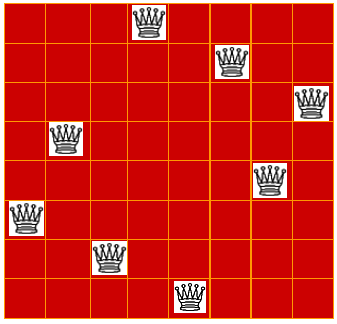
\includegraphics[width=0.35\textwidth]{reinas}
\caption{Posible solución al problema: (4,6,8,2,7,1,3,5)}
\end{figure}

\section{\textcolor{electricgreen}Espacio de soluciones:\\ Organización del Árbol}

\subsection{\textcolor{electricgreen}Terminología}

Los diferentes tipos de árboles que existen en este tipo de problemas los podemos encontrar en \hyperref[arboles]{aquí}. En este tipo de problema, según vaya avanzando el algoritmo, nos podemos encontrar con distintos estados, que tienen una terminología asociada:

\begin{description}
    \item [Estado del problema:] Cada uno de los \textbf{\textcolor{electricgreen}{nodos del árbol}}.
    \item [Estado solución:] Son aquellos nodos $S$ del problema (árbol) \textbf{\textcolor{electricgreen}{para los que el camino desde la raíz a $\mathbf{S}$ representa una $\mathbf{n-}$tupla}} en el espacio de solución.
    \item [Estados respuesta:] Son aquellos estados solución $S$ que representan una $n-$tupla del conjunto de soluciones del problema (aquellas que satisfacen las restricciones implícitas).
\end{description}

\subsection{\textcolor{electricgreen}Generación de estados de un problema}

Cuando sabemos cómo será el árbol de estados del problema, podemos resolver el problema generando estados, determinando cuales de ellos son solución y finalmente, cuales de estos estados solución son estados respuesta.

\subsubsection{\textcolor{electricgreen}Terminología}

\begin{description}
    \item [Nodo vivo:] Estado del problema que ya ha sido generado, pero que aún no se han generado todos sus hijos.
    \item [Nodo muerto:] Estado del problema que ya ha sido generado, y o bien se ha podado o se han generado todos sus hijos.
    \item [$E$-nodo (nodo de expansión):] Nodo vivo que actualmente se están generando los descendientes.
\end{description}

\subsubsection{\textcolor{electricgreen}Generación de estados de un problema}

Hay dos formas de generar estados nuevos en el árbol de soluciones,  las cuales parten del nodo raíz y generan otros nodos, ademas de tener que ir listando los nodos vivos en la \textbf{\textcolor{electricgreen}lista de nodos vivos}.

\begin{description}
    \item [Primer método:] tan pronto como un nuevo hijo $C$ del $E-$nodo en curso $R$ ha sido generado, este \textbf{\textcolor{electricgreen}{hijo se convierte en un nuevo \textit{E-}nodo}}.
    \begin{enumerate}[---]
        \item $R$ se convertirá de nuevo en $E-$nodo cuando el subárbol $C$ haya sido explorado completamente.
        \item Los nodos se generan de la misma forma en la que haríamos un recorrido en profundidad.
    \end{enumerate}
    Se usan \textbf{\textcolor{electricgreen}{funciones de acotación}} para matar nodos vivos sin tener que generar todos sus nodos hijos. Esto es \textbf{\textcolor{electricgreen}{Backtracking}}.

    \item [Segundo método:] el $E-$nodo permanece como $E-$nodo hasta que se hace nodo muerto. Al igual que antes, se usarán funciones de acotación para podar el árbol.

    Este método se adapta muy bien a la resolución de problemas de optimización combinaciones, aquellos que tienen un espacio de soluciones discreto, como pueden ser el problema de la mochila, soluciones enteras, etc.

    Esta forma de exploración es conocida como \hyperref[branchandbound]{Branch \& Bound}
\end{description}

\section{\textcolor{electricgreen}Implementación de Backtracking}

Vamos a suponer lo siguiente antes de presentar la implementación:
    
\begin{enumerate}[---]
    \item Hay que encontrar todos los nodos respuesta.
    \item Sea $(x_1,x_2,\ldots,x_i)$ es un camino desde la raíz hasta un nodo en el árbol de estados.
    \item Sea $T(x_1,x_2,\ldots,x_i)$ el conjunto de todos los posibles valores $x_{i+1}$ tales que $(x_1,x_2,\ldots,x_{i+1})$ es también un camino hacia un estado del problema.
    \item Suponemos la existencia de funciones de acotación que nos podarán la rama $(x_1,x_2,\ldots,x_i)$ si el camino no puede extenderse para alcanzar un nodo respuesta.
    \item Así los candidatos para la posición $i+1$ del vector solución $X(1..n)$ son aquellos valores que son generados por $T$ y satisfacen $B_{i+1}$
\end{enumerate}

\begin{minted}[linenos, mathescape]{pascal}
function Backtrack(n)
    k := 1;
    while k > 0 do
        if QuedanNodos(k) and B(k) then     // queda algún X(k) no probado 
            if camino(X(1),...,X(k)) then   // tal que $X(k) \in T(X(1),\ldots,X(k-1))$ 
                print(X(1),...,X(k))        // y $B_k(X(1),\ldots,X(k)) = true$
                k := k + 1;
        else
            k := k - 1;
        end
    end
end
\end{minted}

\subsection{\textcolor{electricgreen}Eficiencia de Backtracking}

La eficiencia de este tipo de algoritmos depende del tiempo necesario para generar el siguiente estado,del número de $X(k)$ que satisfagan las restricciones explícitas, el tiempo para acotar y el número de $X(k)$ que satisfagan las $B_i \forall i$.

Las funciones de acotación serán buenas cuando poden de forma considerable el árbol, ya que sino, lanzar Backtracking y un algoritmo de fuerza bruta, será en la práctica lo mismo.

Este tipo de funciones, si son buenas, consumen mucho tiempo, por lo que hay que buscar un equilibrio entre la reducción de nodos y el tiempo de computación.

Este último factor es el más determinante, ya que este tipo de algoritmos podría generar sólo $O(n)$ nodos, mientras que si la poda no fuera buena, y el espacio de soluciones fuera muy grande como $2^n$ o $n!$, el tiempo en el peor caso sería de $O(p(n)2^n)$ u $O(q(n)n!)$.

De aquí la importancia de buenos algoritmos de poda, para evitar recorrer espacios muy grandes.


\chapter{\textcolor{coquelicot}Branch \& \textcolor{coquelicot}Bound}
\label{branchandbound}

Esta técnica es muy similar a la técnica de \hyperref[backtracking]{Backtracking} vista anteriormente, y su diseño se basa en el análisis del árbol de estados del problema. Es decir:

\begin{enumerate}[---]
    \item Realiza un recorrido sistemático de ese árbol.
    \item Este recorrido no tiene por qué ser precisamente en profundidad.
\end{enumerate}

Es una técnica que se usa para problemas de optimización y juegos, pero que en el peor de los casos, puede suponer una eficiencia de orden exponencial o peor. Pero, en casos muy grandes, ha demostrado tener un funcionamiento eficiente.

Es básicamente una mejora de Backtracking, donde tendremos una \textcolor{coquelicot}{estrategia de ramificación}, las \textcolor{coquelicot}{técnicas de poda}, para podar nodos rápidamente. La poda se realiza estimando en cada nodo las \textbf{\textcolor{coquelicot}{cotas}} del beneficio estimado que podemos obtener. Esto nos servirá para ramificar el árbol por las ramas más prometedoras.

Las principales diferencias están en que Branch\&Bound no utiliza la búsqueda en profundidad, sino que, se generan todos los hijos del nodo en curso antes de que otro nodo vivo pase a ser el nuevo nodo en curso. Lo que quiere decir, que puede haber más de un nodo vivo a la vez, teniendo que almacenarlos en \textbf{\textit{\textcolor{coquelicot}{lista de nodos vivos (LNV)}}}.

Cuando empezamos un problema, antes de desplegar nodos en el árbol, se debe acotar el beneficio de la mejor solución alcanzable \textbf{\textcolor{coquelicot}M}.

Para cada nodo $i$ tendremos:

\begin{enumerate}[---]
    \item \textbf{CS(i): Cota superior} del beneficio (o coste) óptimo que podemos alcanzar a partir del nodo \textbf{i}.
    \item \textbf{CI(i): Cota inferior} del beneficio (o coste) óptimo que podemos alcanzar a partir del nodo \textbf{i}.
    \item \textbf{BE(i): Beneficio estimado} (o coste) óptimo que se puede encontrar a partir del nodo \textbf{i}.
\end{enumerate}

Estas cotas deben ser fiables, para poder determinar cuándo se puede realizar una poda, mientras que el coste estimado ayuda a decidir qué parte del árbol evaluar primero.

\subsubsection{\textcolor{coquelicot}Estrategia de poda}

Suponiendo un problema de maximización, la estrategia de poda se basará en que un nodo podrá ser podado si:

\begin{enumerate}[---]
    \item $\mathbf{CS(i)\leq CI(j)}$, para algún nodo $j$ generado.
    \item $CS(i) \leq Valor(s)$, para algún nodo $s$ solución final.
\end{enumerate}

Para la implementación, tendremos que usar una variable de poda $C$, que será:

$$ C = max(\{\mathbf{CI(j)~|~\forall~\mathbf{j}~\text{generado}}\},~\{Valor(s)~|~\forall~\mathbf{s}~solución~final\})$$

Teniendo esto, la poda de un nodo $i$ se hará si $\mathbf{CS(i)\leq C}$.

\subsubsection{\textcolor{coquelicot}Estrategias de ramificación}

Al igual que en Backtracking, se hace un recorrido en el árbol de soluciones, pero este recorrido puede ser en profundidad,anchura, según el beneficio estimado, etc.

Sea cual sea el recorrido, tendremos que mantener nuestra lista de nodos vivos, que contiene todos los nodos que han sido generados pero que no han sido explorados todavía. Son los nodos pendientes de tratar por el algoritmo.

La idea básica del algoritmo consiste en sacar un elemento de la lista $LNV$, generar sus descendientes y si no se podan, meterlos en la $LNV$. Pero ahora, surge una nueva pregunta, ¿en qué orden se sacan y se meten los nodos de la lista? Pues esto es algo que depende del tipo de problema o de cómo queramos que se maneje la lista, ya que variará el recorrido que hagamos sobre el árbol.

\begin{description}
    \item [Estrategia de ramificación FIFO (First-In-First-Out):] la $LNV$ se comportará igual que una \textbf{\textcolor{coquelicot}cola} (el primero en llegar, el primero en ser servido) y puede generar recorridos en profundidad, en anchura, o entre otros.
    \begin{figure}[!h]
        \centering
        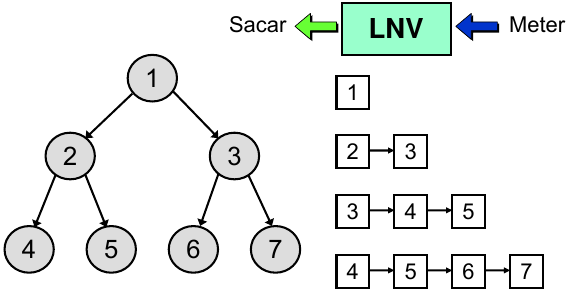
\includegraphics[width=0.6\textwidth]{fifo}
    \end{figure}
    \item [Estrategia de ramificación LIFO (Last-In-First-Out):] en este caso, la $LNV$ se comportará como una \textbf{\textcolor{coquelicot}pila} y el recorrido será parecido al método anterior.
    \begin{figure}[!h]
        \centering
        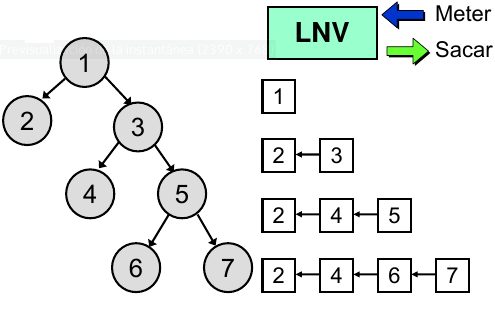
\includegraphics[width=0.6\textwidth]{lifo}
    \end{figure}

    Ambas estrategias hacen búsquedas ``a ciegas'', es decir, no tienen en cuenta los beneficios de los nodos, cotas... Existen otras estrategias que sí tienen en cuenta estas cotas y exploran primero los nodos con mayor beneficio, menor coste...

    \item [Estrategias LC (Least Cost):] Entre todos los nodos vivos de la lista, elegiremos el que tenga mayor beneficio o mínimo coste para seguir explorando.
    \begin{figure}[!h]
        \centering
        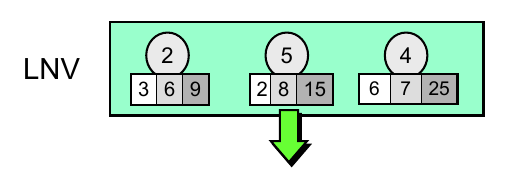
\includegraphics[width=0.6\textwidth]{lc}
    \end{figure}
    \begin{enumerate}[---]
        \item \textbf{Estrategia LC-FIFO}: Seleccionar de la $LNV$ el nodo que tenga mayor beneficio y en caso de empate escoger el primero que se introdujo.
        \item \textbf{Estrategia LC-LIFO}: Seleccionar el nodo que tenga mayor beneficio y en caso de empate, coger el último que entró en la lista.

        Entre estos dos métodos, no hay mucha diferencia, pero, generalmente la estrategia $LC-LIFO$ suele producir mejores resultados.
        \begin{figure}[!h]
            \centering
            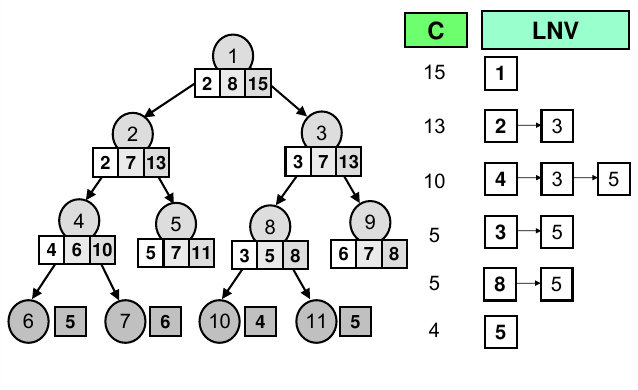
\includegraphics[width=0.6\textwidth]{ej_lifo}
        \end{figure}
    \end{enumerate}
\end{description}

\subsubsection{\textcolor{coquelicot}Implementación de Branch\&Bound}

Esta es la implementación del algoritmo en el caso de minimización:
\begin{minted}[linenos, mathescape]{pascal}
function BranchAndBound(raiz:Nodo; var s:Nodo)
    LNV := {raiz};
    C := CS(raiz);
    s := 0;
    while LNV distinct 0 do
        x := Seleccionar(LNV);   // Estrategia de ramificación
        LNV := LNV - {x};        // Se quita $x$ de la lista
        if CI(x) < C then
            for each y in x.Hijos() do   // Para cada hijo $y$ de $x$
                if Solucion(y) and (Valor(y) < Valor(s)) then
                    s := y;
                    C := min(C,Valor(y));
                elsif not Solucion(y) and (CI(y) <= C) then
                    LNV := LNV + {Y};
                    C := min(C, CS(y));
                endif
            end
        end
    end
end
\end{minted}

\textbf{\textcolor{coquelicot}Funciones utilizadas}
\begin{enumerate}[---]
    \item \textbf{CI(i), CS(i), CE(i)}. Cota inferior, superior y coste estimado.
    \item \textbf{Solucion(x)}. Determina si $x$ es una solución final válida.
    \item \textbf{Valor(x)}. Valor de una solución final.
    \item \textbf{Seleccionar(LNV):Nodo}. Extrae un nodo de la $LNV$ según la estrategia de ramificación.
    \item \textbf{for each y in x.Hijos() do}. iterador para generar todos los descendientes de un nodo.
\end{enumerate}

Un nodo del árbol será una estructura donde guardaremos información sobre el estado en el que se encuentra como puede ser la tupla que da lugar a este estado, nivel, etc., quedando algo así:

\begin{minted}[linenos]{pascal}
Nodo = registro
    tupla:TipoTupla;       // Puede ser un array [1..n] de enteros
    nivel:int;
    CI, CE, CS : double;
end
\end{minted}

\section{\textcolor{coquelicot}Descripción General del Método}

Branch\&Bound explora un árbol comenzando por la raíz o estado original del problema con su región factible, entonces, se estimarán las cotas necesarias para el problema. Si estas cotas cumplen con el objetivo del problema, se haya una solución y se para.

Si se encuentra una solución optimal para un subproblema, será una solución factible para el problema completo, pero no el óptimo global, es decir, que puede haber soluciones con mayor beneficio.

Cuando en un nodo la cota local es peor que el mejor valor conocido, no puede existir un óptimo global en el subespacio que se encuentra. Es decir, si la mejor de las cotas es peor que el valor de la cota $C$, se poda porque no se puede encontrar una solución mejor.

La búsqueda sigue hasta que se examinan o podan todos los nodos, o hasta que se alcanza algún criterio pre-establecido sobre el mejor valor encontrado y las cotas locales de los subproblemas no resueltos.

\subsection{\textcolor{coquelicot}Estimadores y cotas en Branch\&Bound}

\begin{description}
    \item [Cota local:] Se calcula para cada nodo $i$ de forma local. El mejor beneficio que se puede obtener en función del problema se optiene con $LOptimo(i)$ y cuanto mejor o igual sea el valor de la cota local a este valor, mejor será la cota y más se podará.

    \item [Cota global:] Es el valor de la mejor solución estudiada hasta el momento y debe ser peor o igual al beneficio de la solución óptima. Gracias a la velocidad de los algoritmos Greedy, podemos hacer uso de ellos para asignarle unas cotas iniciales. Al igual que antes, cuanto más cercano al óptimo, mejor.

    \item [Estimador del coste/beneficio local óptimo:] Se calcula para cada nodo $i$ y sirve para determinar el siguiente nodo a expandir. Es un estimador como la cota local, pero no tiene por qué ser mejor o igual que $LOptimo(i)$. Es decir, que no importa que si es mejor o peor que este coste, pero puede ser más interesante usar este estimador para determinar qué nodo continuar expandiendo.

    \item [Estrategia de poda:] los nodos que no cumplan las condiciones del problema (restricciones implícitas) deben ser podados; pero, también deben ser podados aquellos nodos que tengan su cota local peor que la cota global. Es decir, si lo mejor que vamos a conseguir por esta rama es peor que lo que ya tenía, se poda.

    No se pierde ninguna solución óptima, ya que si se cumple que $CotaLocal(i) \ge LOptimo(i)$ y $CotaGlobal \leq Óptimo$ entonces $LOptimo(i)$ tiene que ser peor que $Óptimo$ cuando $CotaLocal(i) \leq CotaGlobal$.
\end{description} 

Los criterios de poda sólo se comprueban cuando se introduce un nodo en la $LNV$ o cuando se saca de ella, y si un nodo es solución final entonces no se introduce en la $LNV$, se comprueba si es mejor solución que la actual y se actualiza el valor de $C$.

\subsubsection{\textcolor{coquelicot}Minimización y Maximización}

Ambos problemas se abordan con este tipo de técnicas, y ambas siguen el esquema general del algoritmo, aunque con algunas diferencias:

\begin{description}
    \item [Minimización]:
    \begin{enumerate}[---]
        \item La cota local es una cota inferior $CI(i)$ del mejor coste que se puede conseguir al expandir el nodo $i$, y se debe cumplir:$CI(i) \leq LOptimo(i)$.
        \item La coga global es una cota superior $CS$ del coste del óptimo global, y se debe cumplir que $CS \ge Óptimo$.
        \item La poda se realizará cuando la cota inferior de un nodo $i$ sea mayor que la cota superior.
    \end{enumerate}
    \item [Maximización]:
    \begin{enumerate}[---]
        \item La cota local es una cota superior $CS$ del máximo beneficio que se puede conseguir al expandir el nodo $i$ y se debe cumplir que $CS(i) \ge LOptimo(i)$.
        \item La cota global es una cota inferior $CI$ del beneficio del óptimo global, y se debe cumplir que $CI(i) \leq Optimo$.
        \item La poda se hace cuando $CS(i) < CI$.
    \end{enumerate}
\end{description}

\section{\textcolor{coquelicot}Análisis de la eficiencia}

EL tiempo de ejecución depende principalmente del número de nodos recorridos, es decir, de la efectividad de la poda y del tiempo gastado en cada nodo calculando cotas; además del manejo que se le de a la $LNV$.

En el peor de los casos, haremos un Backtracking ineficiente, porque también tendremos que manejar la lista.

Para hacerlo más eficiente, tenemos que encontrar un punto intermedio entre estimaciones muy precisas que gastan más tiempo de ejecución y aquellas menos precisas pero mucho más rápidas.
%%%%%%%%%%%%%%%%%%%%%%%%%%%%%%%%%%%%%%%%%%%%%%%%%%%%%%%%%%%%%%%%%%%%%%%%%%%%%%%%%%%%%%%%%%%%%%%%%%%%%%%%%%%%%%%%%%%%%%%%%%%%%%%%%%%%%%%%
%                                                           APÉNDICE                                                                    %%%%%%%%%%%%%%%%%%%%%%%%%%%%%%%%%%%%%%%%%%%%%%%%%%%%%%%%%%%%%%%%%%%%%%%%%%%%%%%%%%%%%%%%%%%%%%%%%%%%%%%%%%%%%%%%%%%%%%%%%%%%%%%%%%%%%%%%




































































\appendix
\clearpage
\addappheadtotoc
\appendixpage
\chapter{\textcolor[rgb]{0.1,0.2,1}Eficiencia}
\label{eficiencia}

\section{\textcolor[rgb]{0.1,0.2,1}Ejemplos}

\subsection{\textcolor[rgb]{0.1,0.2,1}Inclusión de límites}
\label{ejem_not}

\begin{multicols}{2}
\subsubsection{$\mathbf{3n^2 \in O(n^2)}$}

Aplicamos la condición de O-grande
\begin{displaymath}
3n^2 \leq c \cdot n^2
\end{displaymath}
Como necesitamos saber el valor exacto de n, lo igualamos
\begin{displaymath}
3n^2 = c \cdot n^2
\end{displaymath}
\begin{displaymath}
3n^2 - c \cdot n^2 = 0
\end{displaymath}
\begin{displaymath}
n^2 \cdot (3 - c) = 0
\end{displaymath}
\begin{displaymath}
n^2 = \frac{0}{3 - c}
\end{displaymath}
Obtenemos como valor de $n$ el cero y como valor de c, un valor que cumpla la condición de ser menor que tres.
\begin{displaymath}
n = 0, c < 3
\end{displaymath}

\subsubsection{$\mathbf{3n^2 \in \Omega(n^2)}$}

Aplicamos la definición de $\Omega$
\begin{displaymath}
3n^2 \geq c \cdot n^2
\end{displaymath}
Igualamos para obtener el valor exacto
\begin{displaymath}
3n^2 \leq c \cdot n^2
\end{displaymath}
\begin{displaymath}
3n^2 = c \cdot n^2
\end{displaymath}
\begin{displaymath}
3n^2 - c \cdot n^2 = 0
\end{displaymath}
\begin{displaymath}
n^2 \cdot (3 - c) = 0
\end{displaymath}
\begin{displaymath}
n^2 = \frac{0}{3 - c}
\end{displaymath}
Obtenemos como valor de $n$ el cero y como valor de c, un valor que cumpla la condición de ser menor que tres.
\begin{displaymath}
n = 0, c < 3
\end{displaymath}

\subsubsection{$\mathbf{3n^2 \in \Theta(n^2)}$}


Como en los dos casos anteriores se cumple la condición, $3n^2 \in \Theta(n^2)$ es cierto en este caso.

\subsubsection{$\mathbf{2^{n+1} \in O(2^n)}$}

\begin{displaymath}
2^{n+1} \leq c \cdot 2^{n}
\end{displaymath}
Vamos a realizar un cambio de variable para despejar la constante $c$
\begin{displaymath}
m = 2^n \qquad 2 \cdot m = c \cdot m
\end{displaymath}
\begin{displaymath}
2 = c
\end{displaymath}
La constante de la función será 2 en este caso, y ahora vamos a calcular el valor de $n$, sustituyendo $c$ por su valor.
\begin{displaymath}
2^{n+1} = 2 \cdot 2^n
\end{displaymath}
\begin{displaymath}
n = 0
\end{displaymath}

\subsubsection{$\mathbf{O(n) \in O(n^2)}$}

Realizamos el límite entre ambas funciones:
\begin{displaymath}
\lim_{n \rightarrow \infty} \frac{n}{n^2} = 0
\end{displaymath}
Como sale cero, nos fijamos en la regla de relación límites/órdenes que dice que
\begin{displaymath}
\lim_{n \rightarrow \infty} \frac{f(n)}{g(n)} \Longrightarrow O(f) \subset O(g)
\end{displaymath}
Y en la regla de relación pertenencia/contenido que dice que
\begin{displaymath}
O(f) \subseteq O(g) \Longleftrightarrow f \in O(g)
\end{displaymath}
Y concluímos que $O(n)$ está incluído en $O(n^2)$.

\subsubsection{$\mathbf{n^2 \in O(n^3)}$}


Siguiendo las reglas de O-grande, $n^2$ está incluido en $O(n^3)$.

\begin{tikzpicture}[scale=0.65]
\begin{axis}[
    axis lines = left,
    xlabel = $n$,
    ylabel = {$R$},
]
%Below the red parabola is defined
\addplot [
    domain=0:20,
    samples=100,
    color=red,
]
{x^2};
\addlegendentry{$f(n)=n^{2}$}
%Here the blue parabloa is defined
\addplot [
    domain=0:20,
    samples=100,
    color=blue,
    ]
    {x^3};
\addlegendentry{$g(n)=n^3$}

\end{axis}
\end{tikzpicture}

\subsubsection{$\mathbf{n^2 \in \Omega(n^3)}$}

Como se ve en la gráfica anterior, $n^3$ está muy por encima de $n^2$. Además, si aplicamos la definición de $\Omega$ obtenemos que:
\begin{displaymath}
n^2 \geq c \cdot n^3
\end{displaymath}
\begin{displaymath}
n^2 = c \cdot n^3
\end{displaymath}
¿Por qué valor $c$ multiplicamos $n^3$ para que se convierta en $n^2$?

\subsubsection{$\mathbf{n^2 \in \Theta(n^3)}$}


Como $n^2 \in \Omega(n^3)$ no es cierto, $n^2 \in \Theta(n^3)$ no puede estar incluido en el orden exacto de $n^3$.

\subsubsection{$\mathbf{(2 + 1)^n \in O(2^n)}$}
\label{apartado9}


Es imposible por la siguiente razón

\begin{displaymath}
\lim_{n \rightarrow \infty} \frac{3^n}{2^n} = +\infty
\end{displaymath}

\subsubsection{$\mathbf{(n+1)! \in O(n!)}$}

Al igual que la anterior, no está incluida
\begin{displaymath}
\lim_{n \rightarrow \infty} \frac{(n+1)!}{n!} = +\infty
\end{displaymath}

\subsubsection{$\mathbf{n^3 \in O(n^2)}$}


Si calculamos el límite cuando $n$ tiene a infinito, el resultado de este límite es infinito, por lo que $n^3 \notin O(n^2)$

\begin{displaymath}
\lim_{n \rightarrow \infty} \frac{n^3}{n^2} = +\infty
\end{displaymath}

\subsubsection{$\mathbf{n^3 \in \Omega(n^2)}$}


Como vimos en el apartado anterior, $n^3$ tiene una velocidad de crecimiento mucho mayor que $n^2$, por lo que si $n^3$ no está contenido en $O(n^2)$ es imposible que esté contenido en $\Omega(n^2)$, por lo que $n^3 \notin \Omega(n^2)$

\subsubsection{$\mathbf{n^3 \in \Theta(n^2)}$}


Como $n^3 \notin O(n^2)$ y $n^3 \notin \Omega(n^2)$, $n^3 \notin \Theta(n^2)$ porque estos valores no se incluyen en la intersección de $O(n^2)$ y $\Omega(n^2)$

\subsubsection{$\mathbf{(2+1)^n \in \Omega(2^n)}$}


Como se vio en el \hyperref[apartado9]{apartado \ref*{apartado9}}, $(2+1)^n \notin O(2^n)$, por lo que tampoco estará incluido en el mejor caso, es decir, $(2+1)^n \notin \Omega(2^n)$

\subsubsection{$\mathbf{n^2 \in O(n!!)}$}


Para comprobar si la inclusión es cierta, vamos a realizar el límite cuando $n$ tiende a $\infty$.

\begin{displaymath}
  \lim_{n \rightarrow \infty} \frac{n^2}{n!!} = 0
\end{displaymath}

Como vemos, el resultado es 0, por lo que $n^2 \in O(n!!)$ es cierto.

\end{multicols} 

\subsection{\textcolor[rgb]{0.1,0.2,1}Fibonacci}

Vamos a calcular la eficiencia teórica de un algoritmo para calcular el término n-ésimo de una sucesión. El algoritmo es el siguiente:

\begin{minted}[linenos]{pascal}
function Fibbonacci (N:int):int;
    if N<0 then
        error('No válido')
    case N of
        0, 1: return N
    else
        fnm2:= 0
        fnm1:= 1
        for i:= 2 to N
            fn:= fnm1 + fnm2
            fnm2 := fnm1
            fnm1 := fn
        end
        return fn
    end
end
\end{minted}

En esta función hay varios bloques de código. El primer $if$ realiza operaciones simples, por lo que la eficiencia es $O(1)$, al igual que el segundo bloque.

A continuación, vamos a analizar el $else$ de la función.

\begin{minted}[linenos, 
                mathescape,
                firstnumber=6]{pascal}
fnm2:= 0                    // $O(1)$
fnm1:= 1                    // $O(1)$
for i:= 2 to N              // $O(1)$
    fn:= fnm1 + fnm2    // $O(1)$  |
    fnm2 := fnm1        // $O(1)$  |   $\Rightarrow \sum_{i=2}^{N} 1 = N \in O(n)$
    fnm1 := fn          // $O(1)$  |
end
\end{minted}

De una forma más extensa, este algoritmo se compone de dos bloques, un \textbf{\textcolor[rgb]{0.1,0.2,1}{if}} y un \textbf{\textcolor[rgb]{0.1,0.2,1}{case}}. Para determinar la eficiencia del algoritmo, haremos uso de la \hyperref[reglas_efic]{regla de la suma}, para obtener el máximo de los dos bloques de sentencias.

\begin{displaymath}
    t(N) = t(N<0) + max(t(then), t(else))
\end{displaymath}

El \textbf{\textcolor[rgb]{0.1,0.2,1}{if}} tiene tan solo sentencias elementales que no aportan mucho ($O(n)$) por lo que nos centraremos en el \textbf{\textcolor[rgb]{0.1,0.2,1}{case}}.
\begin{displaymath}
    = 1 + t(else) \Rightarrow t(else) = t(case) \rightarrow 1 + t(else)
\end{displaymath}
\begin{displaymath}
    = 1 + 2 + \sum_{i=2}^{N} 4 = 3 + 4\cdot \sum_{i=2}^{N}1
\end{displaymath}
\begin{displaymath}
    = 3 + 4 \cdot (n - 1) = 4\cdot n - 1
\end{displaymath}
\begin{center}
    entonces    
\end{center}
\begin{displaymath}
    t(n) = 1 + 4\cdot n -1 = 4 \cdot n \in O(n)
\end{displaymath}

\subsection{\textcolor[rgb]{0.1,0.2,1}Recurrencias}

\subsubsection{\textcolor[rgb]{0.1,0.2,1}Recurrencias homogéneas}
\label{recurrencias}

\begin{displaymath}
T(n) \left\{ \begin{array}{ll}
1 \qquad \qquad \qquad \text{si } n \leq 1 \\
1 + T(n-1) \quad \text{  si } n > 1\\
\end{array} \right.
\end{displaymath}

\begin{align}
T(n) = 1 + T(n-1), n > 1; \quad T(0) = T(1) = 1\\
1 + T(n-2) \qquad (n > 2)\\
= 2 + T(n - 3) \qquad (n > 3)\\
= 3 + T(n - 4) \qquad (n > 4)\\
T(n) = i + T(n - i)\rightarrow i = (n - 1)\\
T(n) = (n - 1) + T(1) = n \in O(n)
\end{align}

\subsubsection{\textcolor[rgb]{0.1,0.2,1}Factorial de un número}
\label{ej_factorial}

\begin{minted}[linenos]{c++}
int factorial (int n){ //la eficiencia depende de n
      if (n<=1)
            return 1; //O(1)

      else
            return n*factorial(n-1);
}
\end{minted}

\begin{displaymath}
T(n) = \left\{ \begin{array}{ll}
T(n-1)+1  &  n \geq 2\\
1         &  n \leq 1
\end{array} \right.
\end{displaymath}

\begin{center}
\begin{align}
T(n) = n \cdot T(n - 1), n > 1; \quad T(0) = T(1) = 1\\
T(n) = 1 + T(n-1), \qquad(n \geq 2)\\
T(n-1) = T(n-2) + 1 = T(n) = 1 + 1 + T(n-2) \qquad (n \geq 3)\\
T(n) = T(n - k) + k \rightarrow k = n-1\\
T(n) = (n-1) + T(n - (n-1)) \\
= (n - 1) + 1 = n \in O(n)
\end{align}
\end{center}

\subsubsection{\textcolor[rgb]{0.1,0.2,1}Recurrencias lineales con ecuación característica}
\label{ejemplos_ec_car_lin}

\subsubsection{\textcolor[rgb]{0.1,0.2,1}Ejemplo 1}
\begin{displaymath}
T(n) = \left\{ \begin{array}{lll}
0 & $n = 0$ \\
5 & $n = 1$ \\
3t_{n-1} & \text{en otro caso}
\end{array} \right.
\end{displaymath}
\begin{center}
\begin{displaymath}
    t_n = 3t_{n-1} + 4t_{n-2}
\end{displaymath}
\begin{displaymath}
    t_n - 3t_{n-1} - 4t_{n-2} = 0
\end{displaymath}
En este caso, podemos tomar $t_n$ como $x^n$ para hallar la ecuación característica
\begin{displaymath}
    t_n = x^n \quad k = 2
\end{displaymath}
Realizamos la transformación de la ecuación completa
\begin{displaymath}
    t_n - 3t_{n-1} - 4t_{n-2} \Rightarrow x^n - x^{n-1} - 4 \cdot x^{n-2} = 0
\end{displaymath}
Para quitar dejarlo en forma polinomial lineal, dividimos $x^{n-2}$ y despejamos:
\begin{displaymath}
    x^2 - 3\cdot x - 4 = 0
\end{displaymath}
\begin{displaymath}
    (x+1)(x-4) = 0
\end{displaymath}
Las soluciones son $4^n$ y $-1^n \rightarrow$ combinación lineal.
% \begin{displaymath}
% %         % \left . \begin{array}{l}
% %         %   t_n = c_1(-1)^n + c_2\cdot4^n\\
% %         % \end{array} \right.
%       x
% \end{displaymath}
\end{center}
\subsubsection{\textcolor[rgb]{0.1,0.2,1}Recurrencias no homogéneas}

\begin{displaymath}
T(n) = \left\{ \begin{array}{ll}
1 & \textrm{si $n \le 2$}\\
T(\frac{n}{2}) + \frac{n}{x} + T(\frac{n}{2}) & \textrm{si $n > 2$} \\
\end{array} \right.
\end{displaymath}
\begin{center}
O lo que es lo mismo:
\end{center}
\begin{displaymath}
T(n) = \left\{ \begin{array}{ll}
1 & \textrm{si $n \le 2$}\\
2\cdot T(\frac{n}{2}) + \frac{n}{x} & \textrm{si $n > 2$} \\
\end{array} \right.
\end{displaymath}
\begin{center}
Hacemos un cambio de variable: $2^k = n \rightarrow k = \log_2 n$:
\end{center}
\begin{displaymath}
T(2^k) = 2T(2^{k-1}) + \frac{2^k}{x} \longrightarrow t_k - 2t_{k-1} = \frac{2^k}{x}
\end{displaymath}
\begin{center}
Las raíces del polinomio son $(x-2)^2$ y por tanto, la ecuación característica es:
\end{center}
\begin{displaymath}
p(x) = c_1 \cdot 2^k + c_2 \cdot n 2^k \longrightarrow p(x) = c1 \log_2 n +  c_2 n \log_2 n \in O(n\log n)
\end{displaymath}

\textbf{\textcolor[rgb]{0.1,0.2,1}Obtener la eficiencia del siguiente fragmento de código}

\begin{minted}[linenos]{c++}
void LF (int n, int *s) {
  int i, x, y;

  if (n < 1) s = 1;
  else {
    x = 1;
    for (i=2; i!=n; i++) x = x * i;
    y = 0;
    do {
      y++;
      x = x/4;
    } while (x != 0);
  }
}
\end{minted}

Como tenemos una sentencia \verb*|if-else|, calculamos la eficiencia de ambas por separado y luego aplicamos la regla de la suma.

El \verb*|if| sería $O(1)$.

Ahora bien, en el \verb*|else| tenemos por un lado un bucle \verb*|for| que se ejecuta $n-1$ veces y, por otro lado, un bucle \verb*|do-while| que se ejecuta $\log_4 ((n-1)!) + 1$ veces. Al ser ambos trozos de código independientes aplicamos la regla de la suma para saber cuál es el máximo:

\begin{displaymath}
\lim_{n \rightarrow \infty} \frac{n-1}{\log_4 ((n-1)!) + 1} \rightarrow {\text{Aplicando la aprox. de Stirling}} \rightarrow \frac{n-1}{(n-1)\log_4 ((n-1) - n)} = 0
\end{displaymath}

\begin{center}
\begin{tikzpicture}
\begin{axis}[
    axis lines = left,
    xlabel = $n$,
    ylabel = {$T(n)$},
]
%Below the red parabola is defined
\addplot [
    domain=1:200,
    samples=100,
    color=red,
]
{x-1};
\addlegendentry{$f(n)=n-1$}
%Here the blue parabloa is defined
\addplot [
    domain=1:200,
    samples=100,
    color=blue,
    ]
    {(log10((x-1)!)/log10(4))+1};
\addlegendentry{$g(n)=log_4 ((n-1)!) + 1$}
\end{axis}
\end{tikzpicture}
\end{center}

Por lo que la eficiencia del \verb*|else| sería $O(\log_4 ((n-1)!)$ = $O(n\log n)$ usando la aproximación de Stirling. Aplicando la regla de la suma entre el \verb*|if| y el \verb*|else| concluímos que también sería la eficiencia de toda la función.

\subsubsection{\textcolor[rgb]{0.1,0.2,1}Ecuaciones no homogéneas}

\textbf{\textcolor[rgb]{0.1,0.2,1}Ejemplo 1}

Obtener el orden de eficiencia de la siguiente ecuación recursiva:
\begin{equation*}
T(n) = 
\begin{cases}
1 & \textit{si } n = 1, n = 2 \\
2T\left(\frac{n}{2}\right) + T\left(\frac{n}{4}\right) + n & \textit{otro caso}
\end{cases}
\end{equation*}
% \begin{displaymath}
    
% \end{displaymath}
\begin{center}
    Nos quedamos con la ecuación general y realizamos un cambio de variable para quitarnos los cocientes $$n = 2^{m}, \quad m = \log_2n$$
    $$T(2^m)=2T(2^{m-1})+T(2^{m-2})+2^m \Longrightarrow t_m=2t_{m-1}+2t_{m-2})+2^m$$
    Una vez aquí, ponemos la función en términos de la ecuación característica, la parte homogénea a un lado y la no homogénea a otro, y trabajamos sobre esto.
    $$t_m-2t_{m-1}-2t_{m-2})=2^m$$
    A continuación, resolveremos la parte homogénea de la ecuación:
    $$t_m-2t_{m-1}-2t_{m-2}) = 0 \Longrightarrow x^2 -2x -1$$
    $$2^m \Longrightarrow (x-b)^{d+1}=(x-2)$$
    $$p(m)=(x^2 - 2x -1)(x-2)$$
    $$(x^2 - 2x -1)=\frac{2 \pm \sqrt{4+4}}{2} = 1 \pm \sqrt{2}$$
    $$p(x)=\left[x-(1+\sqrt{2})\right]\left[x-(1-\sqrt{2})\right]\left[x-2\right]$$
    $$t_m = c_1(1+\sqrt{2})^m + c_2(1-\sqrt{2})^m+c_32^m$$
    $$t_n = c_1(1+\sqrt{2})^{\log_2n} + c_2(1-\sqrt{2})^{\log_2n}+c_3n$$
    Ahora, podemos ver que \textbf{no} tenemos una raíz entera, tal y como estamos acostumbrados. Como se puede ver, se tiene un $(1+\sqrt{2})^{\log_2n}$. Para simplificar esto, haremos uso de la siguiente regla de los \textbf{\textit{logarítmos}}:\\

    \begin{tabular}{|p{4cm}|}
    \hline\begin{center}
        \Large{$n^{\log_ab}=b^{\log_an}$}
    \end{center}\\
    \hline
    \end{tabular}

    ~\\
    Aplicando esto, tenemos la siguiente ecuación:
    $$t_n = c_1n^{\log_2(1+\sqrt{2})} + c_2n^{\log_2(1-\sqrt{2})}+c_3n$$
    $$t_n = c_1n^{\log_2(1+\sqrt{2})} + c_2n^{\log_2(1-\sqrt{2})}+c_3n$$
    Como el logarítmo de un número negativo no existe, este ni siquiera nos va a influir en el cálculo de la eficiencia, por lo que lo rechazamos.
    $$t_n = c_1n^{1.26}+c_3n$$
    Vamos a proceder a calcular el valor de las constantes de la ecuación. No hay que fiarse nunca del valor de las constantes y guiarnos por el valor que pueda tomar $n$, ya que la constante que multiplique a $n$, puede ser negativa, no ``influyendo'' en el tiempo de ejecución.
    \begin{displaymath}
        \left\{ \begin{array}{ll}
        T(1) = c_1\cdot 1^{1.26} + c_3 = 1\\
        T(2) = c_1\cdot 2^{1.26} + 2c_3 = 1
    \end{array} \right.
    \end{displaymath}
    \begin{displaymath}
        \left\{ \begin{array}{ll}
        c_1 + c_3 = 1\\
        2.4c_1 + 2c_3 = 1
    \end{array} \right.
        \left\{ \begin{array}{ll}
        c_1 = -2.5\\
        c_3 = 3.5
    \end{array} \right.
    \end{displaymath}
    $$t_n = -2.5n^{1.26}+3.5n \in O(n)$$
\end{center}

\chapter{\textcolor[rgb]{0.1,0.2,1}Ejemplos resueltos}

\section{\textcolor[rgb]{0.1,0.2,1}Eficiencia}

\subsection{\textcolor[rgb]{0.1,0.2,1}Enunciado}

Hallar la eficiencia en el caso promedio del siguiente algoritmo:\\

\begin{minipage}{0.5\textwidth}
\usemintedstyle{rrt}
\begin{minted}
[
linenos,
frame=single,
label={Algoritmo en pseudocódigo},
]
{pascal}
  i:=1
  while i <= n do
    if a[i] >= a[n] then
      a[n]:=a[i]
    end
    i:=i*2
  end
\end{minted}
\end{minipage}
\begin{minipage}{0.5\textwidth}
\begin{minted}
[
frame=single,
label={Algoritmo en C++},
]
{c++}
  int i = 1;
  while (i <= n) {
    if ( a[i] >= a[n] )
      a[n] = a[i];

    i *= 2;
  }
\end{minted}
\end{minipage}

\subsection{\textcolor[rgb]{0.1,0.2,1}Solución}

Para hallar la eficiencia del caso promedio de este algoritmo, haremos uso de las notaciones asintóticas O-grande (en el peor de los casos $\rightarrow O$) y Omega (en el mejor de los casos $\rightarrow \Omega$).

Antes de nada, analizando el algoritmo, podemos ver que hay un bucle $while$, cuya condición de parada es $i \le n$. Lo primero es averiguar cuales son los límites del bucle. Dentro del bucle tenemos una sentencia $if-then$ y una operación $i = i * 2$. Esta operación nos indica que con cada ejecución del bucle, $i$ se incrementa al doble, por lo que el límite del bucle será de orden logarítmico, concretamente $\log_2(n)$, pero como las bases no se tienen en cuenta, se queda como $\log n$.

\begin{displaymath}
  i = 1 \rightarrow 2 \rightarrow 4 \rightarrow \cdots \rightarrow \log_2 n
\end{displaymath}

Ahora que ya sabemos el límite del bucle, vamos a ver cuantas sentencias se repiten en el mejor y peor de los casos:

\begin{description}
  \item [Mejor de los casos]: en el mejor de los casos, $a[i] \ge a[n]$ es cierto en 0 ocasiones, por lo que el número de sentencias que se repiten es:
  \begin{displaymath}
    \underbrace{1}_{i = 1} + \sum_{i = 1}^{\log n} (\underbrace{3}_{if} + \underbrace{2}_{asignaciones} + \underbrace{1}_{while}) = 1 + 6\log n \in \Omega(\log n)
  \end{displaymath}
  \item [Peor de los casos]: en el peor de los casos $a[i] \ge a[n]$ es cierto en todas las ocasiones, por lo que el número de sentencias que se repiten es:
  \begin{displaymath}
    \underbrace{1}_{i = 1} + \sum_{i = 1}^{\log n} (\underbrace{3}_{if} + \underbrace{3}_{then} + \underbrace{2}_{asignaciones} + \underbrace{1}_{while}) = 1 + 9\log n \in O(\log n)
  \end{displaymath}
\end{description}

Una vez hallado los dos casos, a pesar de que coincidan, no podemos asegurar que la eficiencia del caso promedio sea $\Theta(\log n)$. Para hallarlo, tendremos que averiguar e identificar todos los casos posibles. Es decir, desde el mejor de los casos, hasta el peor, pasando por todos los que hay en medio.

Para ello usaremos lo siguiente:

\begin{displaymath}
  t(n) = \sum_{j=0}^{\log n} \text{Prob}\left[\underbrace{a[i]\ge a[n]}_{\text{cierto en }j\text{ ocasiones}}\right] \cdot t\left[\underbrace{a[i]\ge a[n]}_{\text{no cierto en }j\text{ ocasiones}}\right]
\end{displaymath}

Como no podemos calcular la probabilidad de todos los casos, se usará el enfoque de máxima verosimilitud, en el que la probabilidad de ser cierto o no será igual para todos los casos, es decir, todos los casos son equiprobables, simplificando el modelo y facilitando el ajuste.
\begin{center}
\begin{displaymath}
  \sum_{j=0}^{\log n} \frac{1}{\log(n) + 1} \cdot \left [ \underbrace{1}_{i=1} + \underbrace{\sum_{k = 1}^{j}(1 + 3 + 3 + 2)}_{\text{cierto en }j\text{ ocasiones}} + \underbrace{\sum_{k = j + 1}^{\log n}(1 + 3 + 2)}_{\text{no cierto en }j\text{ ocasiones}} \right]
\end{displaymath}

A continuación, vamos a sumar los términos y resolver las sumatorias:
\begin{displaymath}
  \sum_{j=0}^{\log n} \frac{1}{\log(n) + 1}\cdot\left[ 1 + 9j + 6(\log n - j) \right] \quad = \quad \sum_{j=0}^{\log n} \frac{1}{\log(n) + 1}\cdot\left[ 6\log n + 3j + 1 \right]
\end{displaymath}

Como $\frac{1}{\log n + 1}$ no depende de ningún término, lo sacamos fuera de la sumatoria y dividimos la sumatoria por términos:
\begin{displaymath}
  \frac{1}{\log n + 1} \sum_{j = 0}^{\log n} 6\log n + 3j + 1 \quad = \quad \frac{1}{\log n + 1} \left(\sum_{j = 0}^{\log n} 6\log n + \sum_{j = 0}^{\log n} 3j + \sum_{j = 0}^{\log n} 1 \right)
\end{displaymath}

Ahora resolvemos las sumatorias y combinamos los resultados:
\begin{displaymath}
  \frac{1}{\log n + 1} \left(6\log n \cdot \log n + \frac{3(\log n + 1)\log n}{2} + (\log n + 1) \right)
\end{displaymath}
\begin{displaymath}
  \frac{6(\log n)^2}{\log n + 1} + \frac{3(\log n + 1)\log n}{2(\log n + 1)} + \frac{\log n + 1}{\log n + 1}
\end{displaymath}

El siguiente paso es reunir todo en la misma fracción y quitar logaritmos:
\begin{displaymath}
  \frac{12(\log n)^2 + 3(\log n)^2 + 3\log n + 2\log n + 2}{2(\log n + 1)} \quad = \quad \frac{15(\log n)^2 + 5\log n + 2}{2(\log n + 1)} \quad = \quad 
  \frac{\frac{15(\log n)^2}{\log n} + \frac{5\log n}{\log n} + \frac{2}{\log n}}{\frac{2(\log n + 1)}{\log n}}
\end{displaymath}
\begin{displaymath}
  \frac{13\log n + 3 + \frac{2}{\log n}}{2 + \frac{2}{\log n}}
\end{displaymath}

Para hallar la eficiencia en el caso promedio, calculamos el límite cuando n tiende a $\infty$:
\begin{displaymath}
  \lim_{n\rightarrow \infty} \frac{15\log n + 5 + \frac{2}{\log n}}{2 + \frac{2}{\log n}} \quad \Rightarrow \quad \lim_{n\rightarrow \infty} \frac{15\log n + 5 + \cancel{\frac{2}{\log n}}}{2 + \cancel{\frac{2}{\log n}}} \quad 
\end{displaymath}
\begin{displaymath}
 \lim_{n\rightarrow \infty} \frac{15 \log n + 5}{2} \quad \Rightarrow \quad \lim_{n\rightarrow \infty} \log n \in \Theta(\log n)
\end{displaymath}
\end{center}
Como resultado, obtenemos que la eficiencia en el caso promedio es $\mathbf{\Theta(\log n)}$.

\section{\textcolor[rgb]{0.1,0.2,1}Eficiencia 2}

\subsection{\textcolor[rgb]{0.1,0.2,1}Enunciado}

Obtener el orden de eficiencia de la siguiente ecuación recursiva:

\begin{equation*}
t(n) = 
\begin{cases}
1 & \textit{si } n = 1, \\
3t(\frac{n}{2}) + n & \textit{si } n > 1
\end{cases}
\end{equation*}

\subsection{\textcolor[rgb]{0.1,0.2,1}Solución}

\begin{center}
  Para empezar, vamos a quedarnos con la fórmula general para resolver la ecuación:

  \begin{displaymath}
    t(n) = 3t\left(\frac{n}{2}\right) + n
  \end{displaymath}

  Como vemos, la ecuación general es una ecuación lineal no homogénea y lo que haremos a continuación será obtener las raíces de la parte homogénea y la parte no homogénea:

  \begin{displaymath}
    t(n) - 3t\left(\frac{n}{2}\right) = n
  \end{displaymath}
  Para obtener las raíces de la ecuación, haremos el siguente cambio de variable para hacer los cálculos más sencillos:
  \begin{displaymath}
    n = 2^k \qquad \Longrightarrow \quad k = \log_2 n
  \end{displaymath}
  Ahora la ecuación queda así:
  \begin{displaymath}
    t(2^k) - 3t(2^{k-1}) = 2^k
  \end{displaymath}
  Ahora vamos a obtener las raíces de la parte homogénea, olvidándonos de la parte no homogénea de la ecuación ($2^k$):
  \begin{displaymath}
    t(2^k) -3t(2^{k-1}) = 0 \longrightarrow t_k - 3\cdot t_{k-1} = 0 \longrightarrow x - 3 = 0
  \end{displaymath}

  Las ráices de la parte homogénea son $(x-3)$. Ahora, vamos a calcular las raíces de la parte no homogénea, usando el método de la ecuación característica: $a_0x^n + a_1x^{n-1}+\ldots+a_nx^0 = b^n\cdot p(n)$.

  \begin{displaymath}
      b^n\cdot p(n) \Rightarrow 2^k(1)
  \end{displaymath}

  Como en este caso, el polinomio es de grado 0 y $b^n = 2^k$, las raíces de la parte homogénea son $(x-2)$. En conjunto, la ecuación tiene las raíces $(x-3)(x-2) = 0$.A continuación, se deshace el cambio de variable sustituyendo $k$ por $\log_2 n$ quedando lo siguiente:
  \begin{displaymath}
    t(n) = c_1\cdot 3^k + c_22^k
  \end{displaymath}
  \begin{displaymath}
    t(n) = c_1\cdot 3^{\log_2n} + c_22^{\log_2n} \longrightarrow c_1\left(3^{\left(\frac{\log_3n}{\log_32}\right)}\right) + c_2n
  \end{displaymath}
  \begin{displaymath}
    t(n) = c_1\left(3^{\log_3n}\right)^{\left(\frac{1}{\log_32}\right)} + c_2n
  \end{displaymath}
  \begin{displaymath}
    t(n) = c_1\left(n\right)^{\left(\frac{1}{\log_32}\right)} + c_2n
  \end{displaymath}
\end{center}

Una vez resuelta y reducida la ecuación, tenemos que hayar el orden de eficiencia de la ecuación. Siguiendo un primer impulso se puede decir que el orden de eficiencia es $O\left(n\right)^{\left(\frac{1}{\log_32}\right)}$ ya que es el término que crece antes hacia el infinito. Pero hay que tener el cuenta el valor de las constantes que acompañan a cada miembro. Esto es así, porque en caso de que el valor de $c_1$ sea menor o igual que cero, el tiempo que se obtiene es negativo cosa que en la práctica es imposible. Vamos a comprobar el valor de $c_1$ y $c_2$, pero con la peculiaridad de que no podemos usar el caso base de la ecuación ya que no representa el tiempo de ejecución real para nuestro caso base, ya que este tiempo depende de factores externos al algoritmo, como pueden ser el sistema operativo que ejecute el algoritmo, las características de la máquina, de los datos$\ldots$, Por lo que para obtener si las constastes son positivas o negativas, lo haremos sustituyendo las soluciones en la ecuación general:
\begin{center}
\begin{displaymath}
  n = t(n) - 3t\left(\frac{n}{2}\right)
\end{displaymath}
Teniendo en cuenta que $\left(\frac{1}{2}\right) = \frac{1}{3}$:
\begin{displaymath}
  n = t(n) - 3t\left(\frac{n}{2}\right)
\end{displaymath}
\begin{displaymath}
  n = \left(\cancel{c_1n^{\left(\frac{1}{\log_32}\right)}} + c_2n\right) - 3t\left(\cancel{c_1n^{\left(\frac{1}{\log_32}\right)}} + c_2n\right)
\end{displaymath}
\begin{displaymath}
  n = c_2n -3c_2\frac{n}{2} \quad = \quad c_2n\left(1 - \frac{3}{2}\right) \quad = \quad -c\frac{n}{2}
\end{displaymath}
\begin{displaymath}
  n = -c\frac{n}{2} \longrightarrow c_2 = -2
\end{displaymath}
\end{center}

Como hemos podido comprobar, $c_2$ es negativo, por lo que el valor de $c_1$ tiene que ser positivo, ya que de no ser así, el tiempo de ejecución sería cada vez menor hasta que pasara a ser negativo, cosa que en la práctica es imposible. Por lo que el orden de eficiencia de esta ecuación es $O(n^{\log_23})$

\section{\textcolor[rgb]{0.1,0.2,1}Divide y \textcolor[rgb]{0.1,0.2,1}Vencerás}

\subsection{\textcolor[rgb]{0.1,0.2,1}Enunciado}

Implementar el algoritmo de la multiplicación clásica de enteros largos y la versión que implementa el algoritmo de \textit{\textcolor[rgb]{0.1,0.2,1}{Divide y Vencerás}} de Karatsuba y Ofman.

\subsection{\textcolor[rgb]{0.1,0.2,1}Solución}

\subsubsection{\textcolor[rgb]{0.1,0.2,1}Algoritmo Clásico}

La solución para este algoritmo lo que hace es realizar la multiplicación que haría cualquier persona a mano, multiplicando cada uno de los dígitos del multiplicador por todos los dígitos del multiplicando, lo que supone una ejecución muy lenta, perteneciente al orden de $O(n^2)$.

\begin{center}
\input{ej_mult.latex}  
\end{center}

Para ello lo que hace es obtener los dos números como argumento del programa, metiendo cada uno de los número en dos listas donde cada nodo de la lista corresponde a un dígito del número. La multiplicación se realiza con bucle anidado, insertando en una lista los dígitos resultantes de la multiplicación.

\mypython[label="MultiplicacionClasica"]{multc.py}

\subsubsection{\textcolor[rgb]{0.1,0.2,1}Algoritmo Divide y Vencerás}

En este caso, empezaremos como antes. Pasaremos los números como argumentos del programa y meterlos en sus listas correspondientes. Tras esto, se llama al método de \verb*|MultiplicaEnterosLargsDYV(n1,n2)| que implementa el método de Karatsuba y Ofman.

Este método consiste en dividir los dos números en dos mitades iguales de números, generando 4 mitades de la misma cantidad de dígitos:

\begin{center}
  \input{division}
  $$u = w \cdot 10^s + x$$
  $$v = y \cdot 10^s + z$$
\end{center}

Con esta división, dividimos los números originales y del problema original obtendremos tres subproblemas aplicando:
\begin{displaymath}
  r = u \cdot v = 10^{2S}\cdot w \cdot y + 10^S \cdot \left[(w - x) \cdot (z-y) + w\cdot y + x\cdot z\right] + x\cdot z
\end{displaymath}


\begin{enumerate}[---]
  \item $m1=w\cdot y$
  \item $m2=(w-x) \cdot (z-y)$
  \item $m3=x\cdot z$
\end{enumerate}

Aplicando esto, hacemos las respectivas divisiones en la función \verb*|MultiplicaEnterosLargsDYV(n1,n2)|, se restan las listas pasando los componentes a número para no tener problemas de signo y se llama de forma recursiva a la función. Una vez llegados al caso base, hacemos la multiplicación básica y empezamos a recomponer la solución sumando las listas y desplazándolas a la izquierda tantas cifras como indique \verb|mitad| y \verb|tam|.

Como comparativa, se puede ver en la figura \hyperref[comparativa]{Figura \ref*{comparativa}} la diferencia de tiempos para un número 514 cifras es:
\begin{center}
\begin{figure}[!h]
\centering
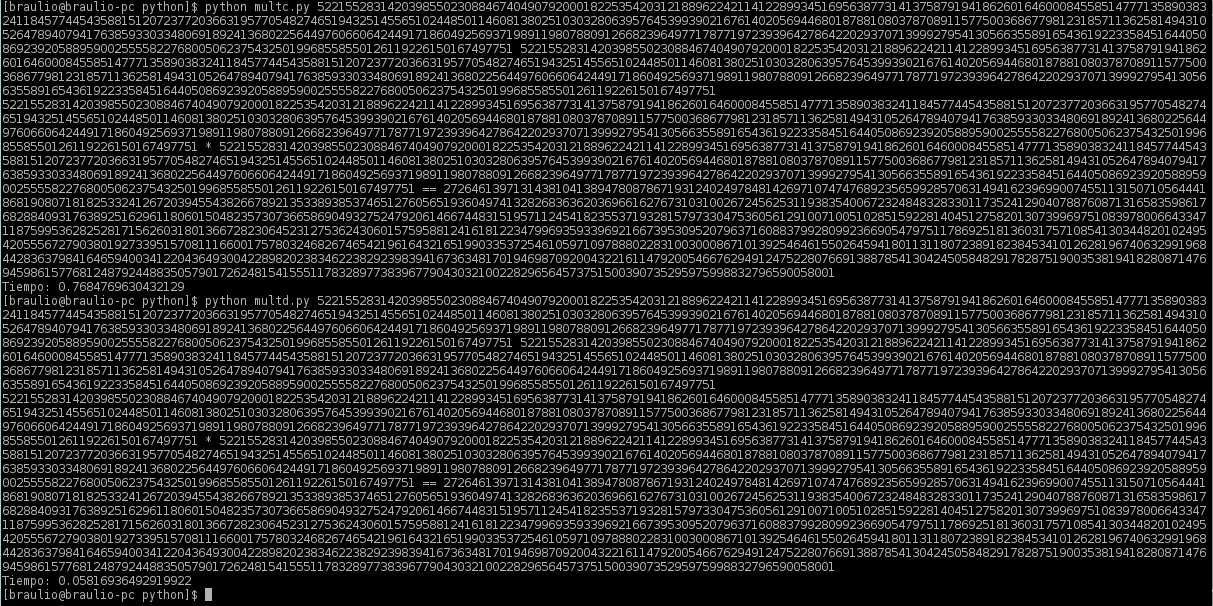
\includegraphics[width=0.8\textwidth]{figura1}
\caption{Alg. clasico = $0.7684769630432129$s. vs. Algoritmo DyV = $0.05816936492919922$s.}
\label{comparativa}
\end{figure}
\end{center}

El algoritmo tiene una orden de eficiencia que viene definido por la siguiente ecuación:
\begin{displaymath}
  t(n) = 3 \cdot t\left(\frac{n}{2}\right)+d'\cdot n
\end{displaymath}

Esta ecuación surge de las tres llamadas recursivas al procedimiento mas la combinación de los resultados. La ecuación del algoritmo pertenece a $O(n^{\log_23}) \approx O(n^{1.59}$. Asintóticamente el algoritmo es mejor, pero para tamaños pequeños, la división en subproblemas y la combinación de los resultados parciales supone que solo haya una mejora para enteros mayores de 500 bits. La \hyperref[figura2]{Figura \ref*{figura2}} es un ejemplo de ello:

\begin{center}
\begin{figure}[!h]
\centering
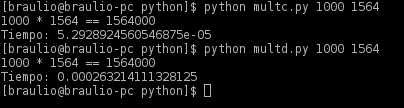
\includegraphics[width=0.44\textwidth]{figura2}
\caption{Alg. clasico = $5.2928924560546875e-05$s. vs. Algoritmo DyV = $0.000263214111328125$s.}
\label{figura2}
\end{figure}
\end{center}

\mypython[label="Karatsuba\&Ofman"]{multd.py}

Como conclusión, el algoritmo solo es rentable para aquellos enteros que son de un tamaño, en la práctica, mayores de $500bits$.

\section{\textcolor[rgb]{0.1,0.2,1}Algoritmos \textcolor[rgb]{0.1,0.2,1}Greedy}

\subsection{\textcolor[rgb]{0.1,0.2,1}Enunciado}

Implementar el problema de la \textbf{\textcolor[rgb]{0.1,0.2,1}{mochila fraccional}} utilizando un \textit{\textcolor[rgb]{0.1,0.2,1}{algoritmo greedy}}.

\subsection{\textcolor[rgb]{0.1,0.2,1}Solución}

Para este problema he propuesto una estructura llamada \verb|objeto| que contiene el \verb|beneficio| y el \verb|peso| de un objeto, donde ambos pueden ser valores reales; y una estructura llamada \verb|Opcion| que recoge el \verb|objeto| y un campo \verb|porcentaje|. Este campo es la proporción del objeto que tomamos.

El algoritmo se basa en de una lista ordenada de \verb|objeto| por beneficio por unidad de peso, escogemos el último ya que la \verb|STL| ordena los elementos de menor a mayor, y lo vamos metiendo en la mochila mientras quede espacio y objetos para meter. Este objeto pasará a ser el que hay en \verb|Opcion.o| y \verb|O.porcentaje = 1|  Una vez que el peso total mas el del objeto que hemos cogido supera el peso de la mochila (y aún queda espacio en la mochila), fraccionamos el objeto con la siguiente razón:
\begin{displaymath}
  porcentaje = \frac{PesoMochila - PesoActual}{PesoDelObjeto}
\end{displaymath}

Esto nos da la proporción del objeto que se mete en la mochila. Tras esto, se iguala el peso actual al peso de la mochila y se sale de la función.
% \newpage
\mycpp[label="MochilaFraccional"]{Greedy.cpp}

% \newpage

A continuación, se muestran dos ejemplos de ejecución para la mochila fraccional para dos ejemplos:

\begin{enumerate}[$\blacksquare$]
  \item El primer ejemplo de ejecución tiene los siguientes datos:
  \begin{enumerate}[$\spadesuit$]
    \item Objetos\footnote{El primer número del objeto indica el beneficio, mientras que el segundo indica el peso de dicho objeto.}: [55, 2], [1,2]
    \item Peso de la mochila: 2.5
  \end{enumerate}
  \item El segundo ejemplo de ejecución tiene:
  \begin{enumerate}[$\spadesuit$]
    \item Objetos: [7, 2], [4, 3], [2, 4], [3, 6]
    \item Peso de la mochila: 11
  \end{enumerate}
\end{enumerate}

\begin{center}
\begin{figure}[!h]
\centering
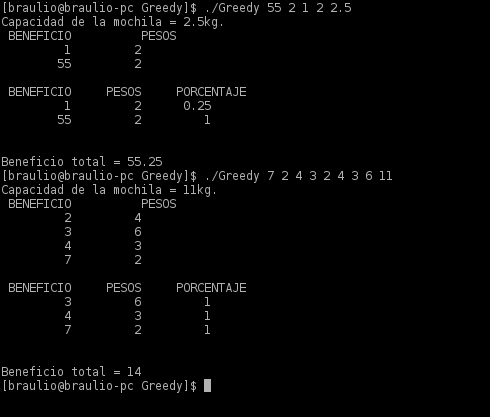
\includegraphics[width=0.5\textwidth]{figura3}
\caption{Ejemplos de ejecución}
\label{figura3}
\end{figure}
\end{center}

\section{\textcolor[rgb]{0.1,0.2,1}Programación Dinámica}

\subsection{\textcolor[rgb]{0.1,0.2,1}Enunciado}

Implementar el problema de la \textbf{\textcolor[rgb]{0.1,0.2,1}{mochila 0/1}} utilizando \textit{\textcolor[rgb]{0.1,0.2,1}{programación dinámica}}.

\subsection{\textcolor[rgb]{0.1,0.2,1}Solución}

Siguiendo la definición del problema de la mochila con la versión para programación dinámica, tenemos los siguientes casos:

\begin{description}
  \item [Si no se coge el objeto $k$]: Nuestra función mochila será la misma pero analizaremoos los $k-1$ objetos restantes.
  $$Mochila(k,m) = Mochila(k-1,m)$$.
  \item [Si se coge:] Nuestra función mochila nos devuelve el beneficio del objeto $k$ mas el beneficio de los $k-1$ objetos restantes.
  $$Mochila(k,m) = b_k + Mochila(k-1, m-p_k)$$
  \item [Valor çoptimo:] El que dé el mayor beneficio:
  $$Mochila(k,mo) = max\{Mochila(k-1,m), b_k + Mochila(k-1, m-p_k)\}$$
\end{description}

Y los siguientes casos base:

\begin{enumerate}[---]
  \item Si $m=0$, no se pueden incluir objetos:
  $$Mochila(k,0) = 0$$
  \item Si $k=0$, tampoco se pueden incluir:
  $$Mochila(k,0) = 0$$
  \item Y si $m$ o $k$ son negativos, tenemos:
  $$Mochila(k<0,m<0) = -\infty$$
  Esto es solo para que cuando uno de los dos sea negativo, directamente se coja la otra opción directamente y no haya problemas en los accesos a memoria en los arrays que conforman la tabla.
\end{enumerate}

Todo esto conforma esta ecuación:

\begin{equation*}
Mochila(k,m)= 
\begin{cases}
0 & \textit{si } k = 0 \textit{ ó } m=0, \\
-\infty & \textit{si } k < 0 \textit{ ó } m < 0, \\
max\{Mochila(k-1,m), b_k + Mochila(k-1, m-p_k)\} &
\end{cases}
\end{equation*}

Siguiendo con esto, rellenamos los casos base de la tabla, que es la fila y columna 0 con 0, y seguimos rellenando la tabla siguiendo la fórmula.

Para recomponer la solución, se utiliza un algoritmo muy sencillo que va recorriendo la tabla desde el final hasta el principio, donde si el elemento que está una fila más arriba del actual es distinto, quiere decir que el objeto se ha cogido y retrocedemos una columna. En caso contrario, seguimos retrocediendo por las filas.

\mycpp[label="Mochila0/1"]{mochila.cpp}

La ejecución del programa da los siguientes resultados:

\begin{center}
\begin{figure}[!h]
\centering
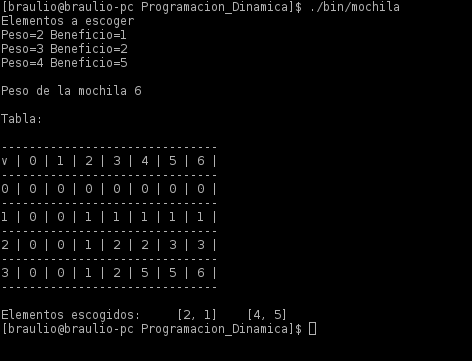
\includegraphics[width=0.8\textwidth]{figura4}
\caption{Ejemplo de ejecución}
\label{figura4}
\end{figure}
\end{center}

\section{\textcolor[rgb]{0.1,0.2,1}Branch\&Bound}
\label{bb}

\subsection{\textcolor[rgb]{0.1,0.2,1}Enunciado}

Implementar el algoritmo de la mochila 0/1 usando un algoritmo \textbf{\textit{\textcolor[rgb]{0.1,0.2,1}}{Branch\&Bound}}.

\subsection{\textcolor[rgb]{0.1,0.2,1}Solución}

Para resolver el ejercicio se ha planteado un árbol binario que coge los elementos del conjunto inicial en un \verb|multiset<Elemento>| ya que inserta los elementos de forma ordenada en función de la proporción de beneficio por unidad de peso y como por debajo tiene un \verb|rb_tree|, el moverse por el conjunto es muy rápido. 

El algoritmo irá cogiendo el último elemento del conjunto (porque la \verb|STL| ordena los elementos de menor a mayor) ya que es el mejor de los objetos posibles e irá generando un árbol binario, analizando primero el coger el objeto y más tarde el de no cogerlo.

Las cotas que se usarán para ramificar y podar son:
\begin{description}
  \item [CI:] Valor actual que llevamos acumulado.
  \item [BE:] Beneficio estimado que calcularemos con un algoritmo Greedy. Este algoritmo greedy recoge el beneficio acumulado que llevemos, mas el beneficio que obtiene cogiendo los mejores objetos que puedan entrar en la mochila, sin pararse a mirar si es conveniente o no.
  \item [CS:] Beneficio que se obtiene sumando el beneficio actual y el beneficio que obtiene el algoritmo greedy en su versión fraccional.
\end{description}

Los nodos pasarán a analizarse si la cota superior es mayor que nuestra cota $C$,que es el valor actual que tenemos. Si es un nodo hoja y su valor es mayor que la cota, se coge el nodo y la tupla asociada. Si aún no es un nodo hoja, se mete en la lista de nodos vivos ($LNV$) para procesarlo más tarde.

El árbol que desarrolla el algorítmo es algo similar a este:

\begin{center}
\begin{figure}[!h]
\centering
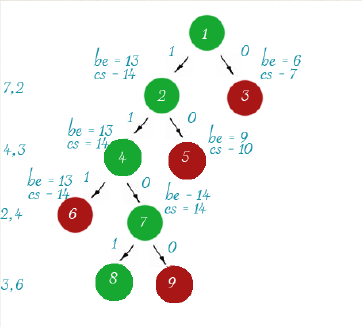
\includegraphics[width=0.6\textwidth]{figura5}
\caption{Árbol binario desarrollado}
\label{figura5}
\end{figure}
\end{center}

\mycpp[label="MochilaBB"]{mochila_branch_bound.cpp}

Un ejemplo de ejecución es el siguiente:

\begin{center}
\begin{figure}[!h]
\centering
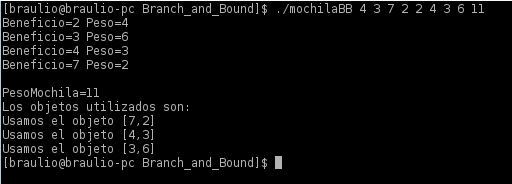
\includegraphics[width=0.5\textwidth]{figura6}
\caption{Ejemplo de ejecución}
\label{figura6}
\end{figure}
\end{center}



\end{document}

%%%%%%%%%%%%%%%%%%%%%%%%%%%%%%%%%%%%%%%%%%%%%%%%%%%%%%%%%%%%%%%%%%%%%%%%%%%%%%%%%%%%%%%%%%%%%%%%%%%%%%%%%%%%%%

\begin{figure}[!h]
\centering
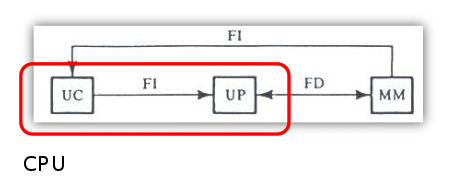
\includegraphics[width=0.5\textwidth]{12}
\caption{asdfsa}
\label{ext2return}
\end{figure}

\hyperref[reglas_efic]{Figura \ref*{reglas_efic}}


\begin{figure}[!h]
\centering
\mbox {
\subfigure[Conteo de los datos]{
\label{conteo}
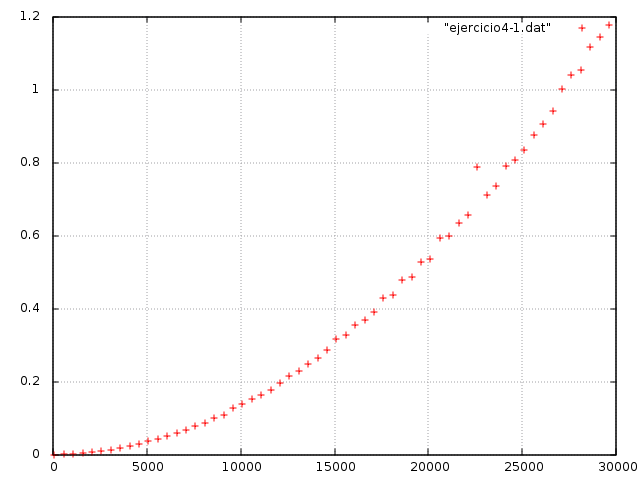
\includegraphics[width=0.4\textwidth]{1}
}
\qquad
\subfigure[Ajuste] {
\label{ajuste}
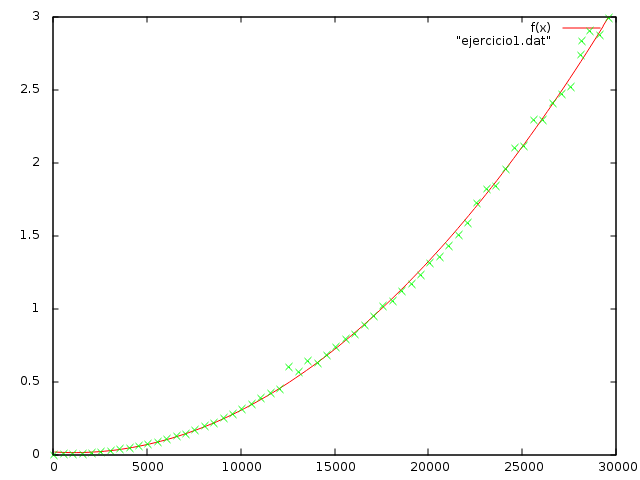
\includegraphics[width=0.4\textwidth]{2}
}
}
\caption{Conteo y ajuste de un estudio a posteriori}
\label{a-post}
\end{figure}


\appendix
\clearpage
\addappheadtotoc
\appendixpage
\section{Lista enteros}
\mycpp[label="ListaEnteros.cpp"]{ListaEnteros.cpp}
\section{Alumnos}
\mycpp[label="Alumnos.cpp"]{alumnos.cpp}
\section{Doble Pila}
\label{pila}
\mycpp[label="DoblePila.h"]{DoblePila.h}
\mycpp[label="DoblePila.cpp"]{DoblePila.cpp}
\section{Matriculas}
\subsection{Clase Matricula}
\label{Matriculas}
\mycpp[label="matricula.h"]{matricula.h}
\mycpp[label="matricula.cpp"]{matricula.cpp}
\subsection{Clase MatriculaAlumnos}
\mycpp[label="MatriculaAlumnos.h"]{MatriculaAlumnos.h}
\mycpp[label="MatriculaAlumnos.cpp"]{MatriculaAlumnos.cpp}














///////////////////////////////////////////////////////////////////////////
ASIGNACIÓN DE TAREAS

\section{\textcolor{electricgreen}Problema de asignación de tareas}

Existen $n$ personas y $n$ trabajos. Cada persona $i$ puede realizar el un trabajo $j$ con más o menos rendimiento: \textbf{B[i,j]}. El objetivo es asignar una tarea a cada trabajador (asignación uno-a-uno), de manera que se maximice la suma de rendimientos.

\begin{description}
    \item [Datos del problema]:
    \begin{enumerate}[---]
        \item \textbf{n}: número de personas y tareas disponibles.
        \item \textbf{B}: \textbf{array}[1..n, 1..n] de enteros. Rendimiento o beneficio de cada asignación. \textbf{B[i,j]} = beneficio de asignar a la persona $i$ la tarea $j$.
    \end{enumerate}
    \item [Resultado]: realizar $n$ asignaciones \{$(p_1,t_1),(p_2,t_2),\ldots,(p_n,t_n)$\}
    \item [Formulación matemática]: maximizar $\sum_{i=1..n}B[p_i,t_i]$, sujeto a la restricción $p_i \neq p_j, t_i \neq t_j, \forall i \neq j$.
\end{description}